\chapter{Confidence intervals}
\label{confidenceIntervals}
\label{sectionConfidenceIntervals}

%\section{Introduction}
%\label{foundationsForInference}




%Statistical inference is concerned primarily with understanding the quality of parameter estimates. For example, a classic inferential question is, ``How sure are we that the estimated mean, $\bar{x}$, is near the true population mean, $\mu$?'' While the equations and details change depending on the setting, the foundations for inference are the same throughout all of statistics. We introduce these common themes in Sections~\ref{variabilityInEstimates}-\ref{cltSection} by discussing inference about the population mean, $\mu$, and set the stage for other parameters and scenarios in Section~\ref{aFrameworkForInference}. Some advanced considerations are discussed in Section~\ref{sampleSizeAndPower}. Understanding this chapter will make the rest of this book, and indeed the rest of statistics, seem much more familiar.

%\index{data!run10|(}

%Throughout the next few sections we consider a data set called \data{run10}, which represents all 16,924 runners who finished the 2012 Cherry Blossom 10 mile run in Washington, DC.\footnote{\urlwofont{http://www.cherryblossom.org}} Part of this data set is shown in Table~\ref{run10DF}, and the variables are described in Table~\ref{run10Variables}.
%
%\begin{table}[h]
%\centering
%\begin{tabular}{rrrrr}
%  \hline
%ID & time & age & gender & state \\ 
%  \hline
%1 & 92.25 & 38.00 & M & MD \\ 
%2 & 106.35 & 33.00 & M & DC \\ 
%3 & 89.33 & 55.00 & F & VA \\ 
%4 & 113.50 & 24.00 & F & VA \\ 
%$\vdots$ & $\vdots$ & $\vdots$ & $\vdots$ & $\vdots$ \\
%16923 & 122.87 & 37.00 & F & VA \\ 
%16924 & 93.30 & 27.00 & F & DC \\ 
%   \hline
%\end{tabular}
%\caption{Six observations from the \data{run10} data set.}
%\label{run10DF}
%\end{table}
%% library(openintro); library(xtable); data(run10); xtable(run10[c(1,2,3,4, nrow(run10)-1:0), c("time", "age", "gender", "state")])
%
%\begin{table}[H]
%\centering\small
%\begin{tabular}{l p{65mm}}
%\hline
%{\bf variable} & {\bf description} \\
%\hline
%\var{time} & Ten mile run time, in minutes \\
%\var{age} & Age, in years \\
%\var{gender} & Gender (\resp{M} for male, \resp{F} for female) \\
%\var{state} & Home state (or country if not from the US) \\
%\hline
%\end{tabular}
%\caption{Variables and their descriptions for the \data{run10} data set.}
%\label{run10Variables}
%\end{table}
%
%%\index{data!run10Samp|(}
%
%These data are special because they include the results for the entire population of runners who finished the 2012 Cherry Blossom Run. We took a simple random sample of this population, which is represented in Table~\ref{run10SampDF}. We will use this sample, which we refer to as the \data{run10Samp} data set, to draw conclusions about the entire population. This is the practice of statistical inference in the broadest sense. Two histograms summarizing the time and age variables in the \data{run10Samp} data set are shown in Figure~\ref{run10SampHistograms}.
%
%\begin{table}
%\centering
%\begin{tabular}{rrrrr}
%  \hline
%ID & time & age & gender & state \\ 
%  \hline
%1983 & 88.31 & 59 & M & MD \\ 
%8192 & 100.67 & 32 & M & VA \\ 
%11020 & 109.52 & 33 & F & VA \\ 
%  $\vdots$~~ &   $\vdots$~~~ &   $\vdots$~ &   $\vdots$~ &   $\vdots$~\, \\ 
%1287 & 89.49 & 26 & M & DC \\ 
%   \hline
%\end{tabular}
%\caption{Four observations for the \data{run10Samp} data set, which represents a simple random sample of 100 runners from the 2012 Cherry Blossom Run.}
%\label{run10SampDF}
%%library(openintro); library(xtable); data(run10); data(run10Samp); xtable(run10Samp[c(1,2,3,100),])
%\end{table}
%
%% WARNING: This figure is referenced in Section 4.2
%\begin{figure}
%\centering
%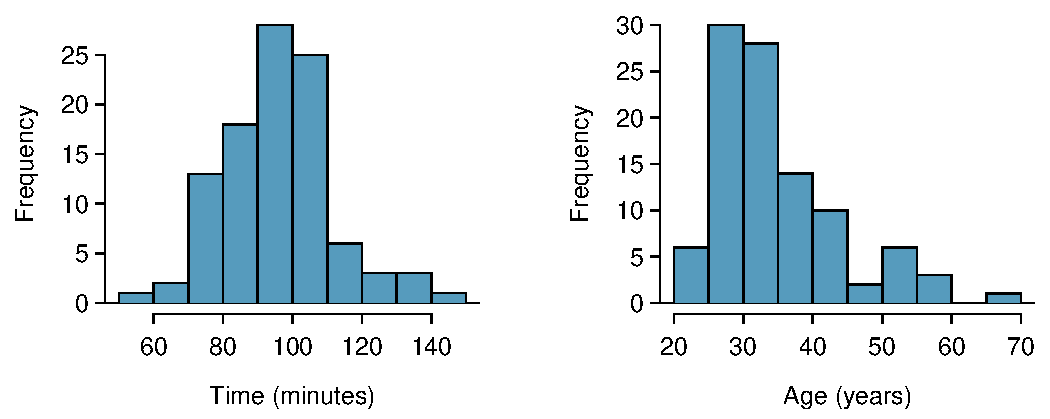
\includegraphics[width=\textwidth]{04-5/figures/run10SampHistograms/run10SampHistograms} 
%\caption{Histograms of \var{time} and \var{age} for the sample Cherry Blossom Run data. The average time is in the mid-90s, and the average age is in the mid-30s. The age distribution is moderately skewed to the right.\index{skew!example: moderate}}
%\label{run10SampHistograms}
%\end{figure}
%
%
%%__________________
%\section{Variability in estimates}
%\label{variabilityInEstimates}
%
%\index{point estimate|(}
%
%We would like to estimate two features of the Cherry Blossom runners using the sample. 
%\begin{itemize}
%\setlength{\itemsep}{0mm}
%\item[(1)] How long does it take a runner, on average, to complete the 10 miles?
%\item[(2)] What is the average age of the runners?
%\end{itemize}
%These questions may be informative for planning the Cherry Blossom Run in future years.\footnote{While we focus on the mean in this chapter, questions regarding variation are often just as important in practice. For instance, we would plan an event very differently if the standard deviation of runner age was 2 versus if it was 20.} We will use $x_1, ..., x_{100}$ to represent the 10 mile time for each runner in our sample, and $y_1, ..., y_{100}$ will represent the age of each of these participants.
%
%\subsection{The problem with point estimates}
%\label{pointEstimates}
%
%\index{point estimate!single mean|(}
%
%We want to estimate the \term{population mean} based on the sample. The most intuitive way to go about doing this is to simply take the \term{sample mean}. That is, to estimate the average 10 mile run time of all participants, take the average time for the sample:
%\begin{eqnarray*}
%\bar{x} = \frac{88.22 + 100.58 + \dots + 89.40}{100} = 95.61
%\end{eqnarray*}
%The sample mean $\bar{x} = 95.61$ minutes a \term{point estimate} of the population mean.
%%if we can only choose one value to estimate the population mean, this is our best guess. 
%Suppose we take a new sample of 100 people and recompute the mean; we will probably not get the exact same answer that we got using the \data{run10Samp} data set. Estimates generally vary from one sample to another, and this \term{sampling variation} suggests our estimate may be close, but it will not be exactly equal to the parameter.
%
%We can also estimate the average age of participants by examining the sample mean of \var{age}:
%\begin{eqnarray*}
%\bar{y} = \frac{59 + 32 + \dots + 26}{100} = 35.05
%\end{eqnarray*}
%%library(openintro); library(xtable); data(run10); data(run10Samp); run10Samp$age[c(1,2,100)]; mean(run10Samp$age); mean(run10$age, na.rm=TRUE)
%
%What about generating point estimates of other \term{population parameters}, such as the population median or population standard deviation? Once again we might estimate parameters based on sample statistics, as shown in Table~\ref{ptEstimatesNetTimeAge}. For example, we estimate the population standard deviation for the running time using the sample standard deviation, 15.78 minutes.
%
%\begin{table}[h]
%\centering
%\begin{tabular}{ l rr}
%\hline
%\resp{time}		& estimate & parameter  \\
%\hline
%mean		& 95.61 & 94.52 \\
%median	& 95.46 & 94.03 \\
%st. dev.		& 15.78 & 15.93 \\
%\hline
%\end{tabular}
%\caption{Point estimates and parameter values for the \var{time} variable.}
%\label{ptEstimatesNetTimeAge}
%\end{table}
%%library(openintro); library(xtable); data(run10); data(run10Samp); d <- run10Samp$time; mean(d); median(d); sd(d); d <- run10$time; mean(d); median(d); sd(d)
%
%
%\begin{exercise} \label{pointEstimateOfDifferentNetTimesBetweenGender}
%Suppose we want to estimate the difference in run times for men and women. If $\bar{x}_{men} = 87.65$ and $\bar{x}_{women} = 102.13$, then what would be a good point estimate for the population difference?\footnote{We could take the difference of the two sample means: $102.13 - 87.65 = 14.48$. Men ran about 14.48 minutes faster on average in the 2012 Cherry Blossom Run.}
%\end{exercise}
%%library(openintro); library(xtable); data(run10); data(run10Samp); (x <- by(run10Samp$time, run10Samp$gender, mean)); diff(x)
%
%\begin{exercise}
%If you had to provide a point estimate of the population IQR for the run time of participants, how might you make such an estimate using a sample?\footnote{To obtain a point estimate of the IQR for the population, we could take the IQR of the sample.}
%
%\index{point estimate!single mean|)}
%
%\end{exercise}
%
%%\subsection{Point estimates are not exact}
%
%Point estimates are usually not exactly equal to the truth, but they get better as more data become available. We can see this by plotting a running mean from our \data{run10Samp} sample. A \term{running mean} is a sequence of means, where each mean uses one more observation in its calculation than the mean directly before it in the sequence. For example, the second mean in the sequence is the average of the first two observations and the third in the sequence is the average of the first three. The running mean for the 10 mile run time in the \data{run10Samp} data set is shown in Figure~\ref{netTimeRunningMean}, and it approaches the true population average, 94.52 minutes, as more data become available.
%
%\begin{figure}[H]
%   \centering
%   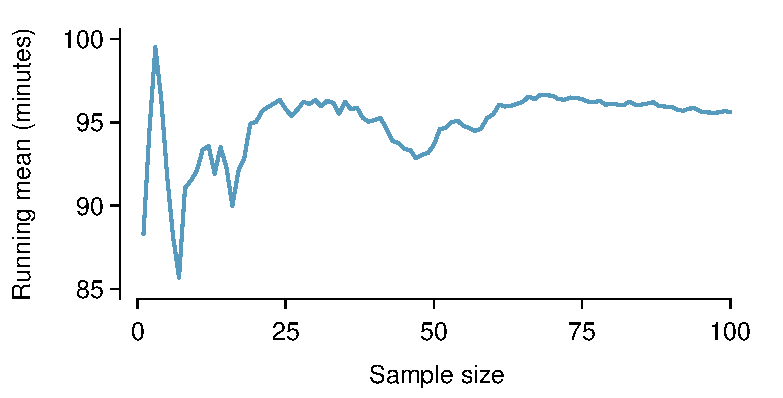
\includegraphics[width=0.7\textwidth]{04-5/figures/netTimeRunningMean/netTimeRunningMean}
%   \caption{The mean computed after adding each individual to the sample. The mean tends to approach the true population average as more data become available.}
%   \label{netTimeRunningMean}
%\end{figure}
%
%Sample point estimates only approximate the population parameter, and they vary from one sample to another. If we took another simple random sample of the Cherry Blossom runners, we would find that the sample mean for the run time would be a little different. It will be useful to quantify how variable
%an estimate is from one sample to another. If this variability is small (i.e. the sample mean doesn't change much from one sample to another) then that estimate is probably very accurate. If it varies widely from one sample to another, then we should not expect our estimate to be very good.
%
%
%\subsection{Standard error of the mean}
%\label{seOfTheMean}
%
%From the random sample represented in \data{run10Samp}, we guessed the average time it takes to run 10 miles is 95.61 minutes. Suppose we take another random sample of 100 individuals and take its mean: 95.30 minutes. Suppose we took another (93.43 minutes) and another (94.16 minutes), and so on. If we do this many many times -- which we can do only because we have the entire population data set -- we can build up a \term{sampling distribution} for the sample mean when the sample size is 100, shown in Figure~\ref{netTime1000SamplingDistribution}.
%
%\begin{figure}
%   \centering
%   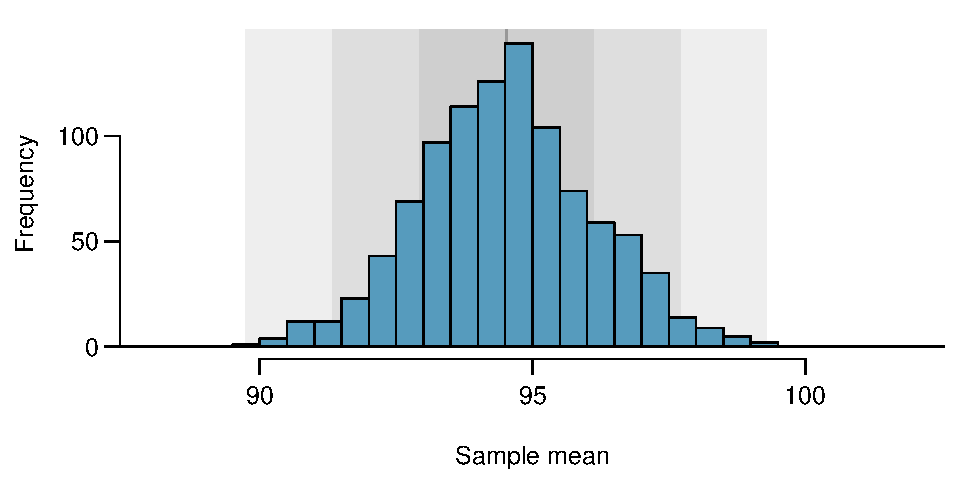
\includegraphics[width=0.85\textwidth]{04-5/figures/netTime1000SamplingDistribution/netTime1000SamplingDistribution}
%   \caption{A histogram of 1000 sample means for run time, where the samples are of size $n=100$.}
%   \label{netTime1000SamplingDistribution}
%\end{figure}
%
%%\begin{termBox}{\tBoxTitle{Sampling distribution}
%%The sampling distribution represents the distribution of the point estimates based on samples of a fixed size from a certain population. It is useful to think of a particular point estimate as being drawn from such a distribution. Understanding the concept of a sampling distribution is central to understanding statistical inference.}
%%\end{termBox}
%
%The sampling distribution shown in Figure~\ref{netTime1000SamplingDistribution} is unimodal and approximately symmetric. It is also centered exactly at the true population mean: $\mu=94.52$. Intuitively, this makes sense. The sample means should tend to ``fall around'' the population mean.
%
%We can see that the sample mean has some variability around the population mean, which can be quantified using the standard deviation of this distribution of sample means: $\sigma_{\bar{x}} = 1.59$. The standard deviation of the sample mean tells us how far the typical estimate is away from the actual population mean, 94.52 minutes. It also describes the typical \term{error} of the point estimate, and for this reason we usually call this standard deviation the \term{standard error (SE)}\index{SE}\marginpar[\raggedright\vspace{-4mm}
%
%$SE$\\\footnotesize standard\\error]{\raggedright\vspace{-4mm}
%
%$SE$\\\footnotesize standard\\error} of the estimate.
%
%\begin{termBox}{\tBoxTitle{Standard error of an estimate}
%The standard deviation associated with an estimate is called the \emph{standard error}. It describes the typical error or uncertainty associated with the estimate.}
%\end{termBox}
%
%When considering the case of the point estimate $\bar{x}$, there is one problem: there is no obvious way to estimate its standard error from a single sample. However, statistical theory provides a helpful tool to address this issue. 
%
%\begin{exercise}
%(a) Would you rather use a small sample or a large sample when estimating a parameter? Why? (b) Using your reasoning from (a), would you expect a point estimate based on a small sample to have smaller or larger standard error than a point estimate based on a larger sample?\footnote{(a) Consider two random samples: one of size 10 and one of size 1000. Individual observations in the small sample are highly influential on the estimate while in larger samples these individual observations would more often average each other out. The larger sample would tend to provide a more accurate estimate. (b) If we think an estimate is better, we probably mean it typically has less error. Based on (a), our intuition suggests that a larger sample size corresponds to a smaller standard error.}
%\end{exercise}
%
%In the sample of 100 runners, the standard error of the sample mean is equal to one-tenth of the population standard deviation: $1.59 = 15.93/10$. In other words, the standard error of the sample mean based on 100 observations is equal to
%\begin{eqnarray*}
%SE_{\bar{x}} = \sigma_{\bar{x}} = \frac{\sigma_{x}}{\sqrt{n}} = \frac{15.93}{\sqrt{100}} = 1.59
%\end{eqnarray*}
%where $\sigma_{x}$ is the standard deviation of the individual observations. This is no coincidence. We can show mathematically that this equation is correct when the observations are independent  using the probability tools of Section~\ref{randomVariablesSection}.
%
%\begin{termBox}{\tBoxTitle{Computing SE for the sample mean}
%Given $n$ independent observations from a population with standard deviation $\sigma$, the standard error of the sample mean is equal to \vspace{-1mm}
%\begin{eqnarray}
%SE = \frac{\sigma}{\sqrt{n}}
%\label{seOfXBar}
%\end{eqnarray}\vspace{-3mm}%
%
%A reliable method to ensure sample observations are independent is to conduct a simple random sample consisting of less than 10\% of the population.\index{standard error!single mean}
%}
%\end{termBox}
%
%There is one subtle issue of Equation~(\ref{seOfXBar}): the population standard deviation is typically unknown. You might have already guessed how to resolve this problem: we can use the point estimate of the standard deviation from the sample. This estimate tends to be sufficiently good when the sample size is at least 30 and the population distribution is not strongly skewed%\footnote{Some books suggest 30 is sufficient; we take a slightly more conservative approach.}
%% x <- c(); for(i in 1:10000){ x[i] <- mean(exp(rnorm(30, sd=0.5))) }; hist(x); (quantile(x, c(0.025, 0.975)) - mean(x)) / sd(x)
%% M <- mean(x); x <- rep(NA, 1000); for(i in 1:1000){ temp <- exp(rnorm(30, sd=0.5)); x[i] <- (max(temp) - M) / sd(temp) }; hist(x); quantile(x, 0.95)
%% for(i in 1:1000){ temp <- exp(rnorm(30, sd=0.5)); hist(temp, breaks=seq(0, 12, 0.5), main=round((max(temp) - mean(temp))/sd(temp), 1)); Sys.sleep(0.5) }
%. Thus, we often just use the sample standard deviation $s$ instead of~$\sigma$. When the sample size is smaller than 30, we will need to use a method to account for extra uncertainty in the standard error. If the skew condition is not met, a larger sample is needed to compensate for the extra skew. These topics are further discussed in Section~\ref{cltSection}.
%
%\begin{exercise}
%In the sample of 100 runners, the standard deviation of the runners' ages is $s_y = 8.97$. Because the sample is simple random and consists of less than 10\% of the population, the observations are independent. (a)~What is the standard error of the sample mean, $\bar{y}=35.05$ years? (b)~Would you be surprised if someone told you the average age of all the runners was actually 36~years?\footnote{(a) Use Equation~(\ref{seOfXBar}) with the sample standard deviation to compute the standard error: $SE_{\bar{y}} = 8.97/\sqrt{100} = 0.90$ years. (b) It would not be surprising. Our sample is about 1 standard error from 36 years. In other words, 36 years old does not seem to be implausible given that our sample was relatively close to it. (We use the standard error to identify what is close.)}
%\end{exercise}
%%library(openintro); library(xtable); data(run10); data(run10Samp); mean(run10Samp$age); sd(run10Samp$age); sd(run10$age, na.rm=TRUE)
%
%
%\begin{exercise}
%(a) Would you be more trusting of a sample that has 100 observations or 400 observations? (b) We want to show mathematically that our estimate tends to be better when the sample size is larger. If the standard deviation of the individual observations is 10, what is our estimate of the standard error when the sample size is 100? What about when it is 400? (c) Explain how your answer to (b) mathematically justifies your intuition in part~(a).\footnote{(a) Extra observations are usually helpful in understanding the population, so a point estimate with 400 observations seems more trustworthy. (b) The standard error when the sample size is 100 is given by $SE_{100} = 10/\sqrt{100} = 1$. For 400: $SE_{400} = 10/\sqrt{400} = 0.5$. The larger sample has a smaller standard error. (c) The standard error of the sample with 400 observations is lower than that of the sample with 100 observations. The standard error describes the typical error, and since it is lower for the larger sample, this mathematically shows the estimate from the larger sample tends to be better -- though it does not guarantee that every large sample will provide a better estimate than a particular small sample.}
%\end{exercise}
%
%%\subsection{Basic properties of point estimates}
%%
%%We achieved three goals in this section. First, we determined that point estimates from a sample may be used to estimate population parameters. We also determined that these point estimates are not exact: they vary from one sample to another. Lastly, we quantified the uncertainty of the sample mean using what we call the standard error, mathematically represented in Equation~\eqref{seOfXBar}. While we could also quantify the standard error for other estimates -- such as the median, standard deviation, or any other number of statistics -- we will postpone these extensions until later chapters or courses.
%
%\index{point estimate|)}












%__________________
%\section{Confidence intervals}
%\label{confidenceIntervals}

\index{confidence interval|(}

A point estimate provides a single plausible value for a parameter. However, a point estimate is rarely perfect; usually there is some error in the estimate. Instead of supplying just a point estimate of a parameter, a next logical step would be to provide a plausible \emph{range of values} for the parameter%.
with a certain amount of confidence.

\begin{termBox}{\tBoxTitle{Confidence Intervals}
%\vspace{-3mm}
A plausible range of values for a  parameter is called a \term{confidence interval}.%
%\vspace{-3mm}
}
\end{termBox}

%The key point to keep in mind is that we don't have a single value anymore as we did with point estimates
%but a range of possible values that we claim capture a target parameter with a certain amount
%of confidence.


%In this section and in Section~\ref{hypothesisTesting}, we will emphasize the special case where the point estimate is a sample mean and the parameter is the population mean. In Section~\ref{aFrameworkForInference}, we generalize these methods for a variety of point estimates and population parameters that we will encounter in Chapter~\ref{inferenceForNumericalData} and beyond.

\section{Introduction}
\label{sectionIntroductionOnCofidenceIntervals}

\subsection{Capturing the population parameter}

Using only a point estimate is like fishing in a murky lake with a spear, and using a confidence interval is like fishing with a net. We can throw a spear where we saw a fish, but we will probably miss. On the other hand, if we toss a net in that area, we have a good chance of catching the fish.
If we report a point estimate, we probably will not hit the exact population parameter. On the other hand, if we report a range of plausible values -- a confidence interval -- we have a good shot at capturing the parameter. 
The idea is to create an interval centered around the point estimate that will capture the parameter with a certain amount of confidence.

\begin{exercise}
If we want to be very certain we capture the population parameter, should we use a wider interval or a smaller interval?\footnote{If we want to be more certain we will capture the fish, we might use a wider net. Likewise, we use a wider confidence interval if we want to be more certain that we capture the parameter.}
\end{exercise}

\subsection{Constructing an approximate $(1-\alpha)$\% confidence interval}
\label{sectionConstructingAnApproximateCConfidenceInterval}

Since our point estimate is the most plausible value of the parameter, so it makes sense to build the confidence interval around the point estimate. The standard error, which is a measure of the uncertainty associated with the point estimate, provides a guide for how large we should make the confidence interval.

Recall that the standard error represents the standard deviation associated with the estimate.
Roughly $(1-\alpha)$\% of the time the estimate will be within a certain number of fixed standard errors of the parameter.
$(1-\alpha)$ is a fixed number that can be found out using a reference distribution such as the standard normal distribution.
If an interval spreads out this fixed number of standard errors from the point estimate, we can be 
approximately 
$(1-\alpha)$\% \term{confident} that we have captured the true parameter
\footnote{This notation might appear strange, but we are in fact using standard notation which will make more sense when we study hypothesis tests in Chapter~\ref{sectionHypothesisTesting}.}.

%\begin{eqnarray}
%\text{point estimate}\ \pm\ 2\times SE
%\label{95PercentConfidenceIntervalFormula}
%\end{eqnarray}
\begin{termBox}{\tBoxTitle{Basic skeleton of a confidence interval}
\vspace{-3mm}
\begin{align}
\text{estimator}	& ~\pm~ 	\underbrace{
					\bigg( \parbox[c]{3.35cm}{ \centering value from a reference distribution } \bigg)
					\times
					\bigg( \parbox[c]{2.70cm}{ \centering standard error of the estimate } \bigg)
						}_{ \text{margin of error} }\label{tboxSkeletonOfCI}
\end{align}\label{95PercentConfidenceIntervalFormula}
\vspace{-3mm}
}
\end{termBox}

Although the construction of a confidence interval has essentially the same basic structure, the  values
that we substitute into~\ref{95PercentConfidenceIntervalFormula} depend on the situation.
The value from the reference distribution multiplied by the standard error of the estimate is called
the \term{margin of error}.
Recall that a confidence interval is a range of values. 
We get the upper bound of the range by adding the margin of error to the estimator and we get the lower bound by subtracting the margin of error from the estimator.
%For example, if we are interested in constructing a confidence interval for the mean when the population
%standard deviation $\sigma$ is known, the estimator is the sample mean $\bar{x}$, 
%the standard error is $\sigma/\sqrt{n}$ (from the Central Limit Theorem in Section~\ref{cltSection})
%and the value from the reference distribution is taken from the standard normal distribution.







\subsection{Interpreting an approximate $(1-\alpha)$\% confidence interval}
\label{interpretingCIs}
\index{confidence interval!interpretation|(}

In Section~\ref{sectionConstructingAnApproximateCConfidenceInterval} we learnt the basic procedure
behind creating a $(1-\alpha)$\% confidence interval.
But what does a ``$(1-\alpha)$\% confident'' mean? 
Let's consider the specific case where $\alpha = 0.05$.
$1 - \alpha = 1 - 0.05 = 0.95$ which means that interested in interpreting a 
95\% confidence interval.
Suppose we took many samples and built a confidence interval from each sample using the appropriate values in Equation~(\ref{95PercentConfidenceIntervalFormula}). Then approximately 95\% of those intervals would contain the actual mean, $\mu$. 
%Figure~\ref{95PercentConfidenceInterval} shows this process with 25 samples, where 24 of the resulting confidence intervals contain the average time for all the runners, $\mu=94.52$ minutes, and one does not.
Figure~\ref{95PercentConfidenceInterval} shows this process with 25 samples.
%\begin{figure}[hht]
\vspace{-7mm}
\begin{figure}[H]
   \centering
   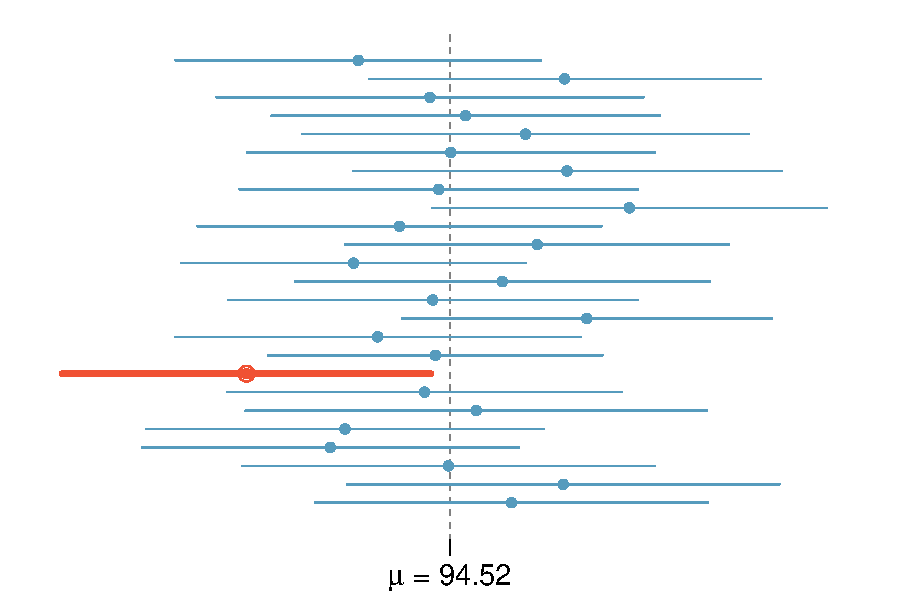
\includegraphics[width=0.66\textwidth]{04-5/figures/95PercentConfidenceInterval/95PercentConfidenceInterval}
%   \caption{Twenty-five samples of size $n=100$ were taken from the \data{run10} data set. For each sample, a confidence interval was created to try to capture the average 10 mile time for the population. Only 1 of these 25 intervals did not capture the true mean which is $\mu = 94.52$ minutes.}
   \caption{25 samples of size $n=100$ were taken from the \data{run10} data set. A 95\% confidence interval for mean time was created with each sample. Only 1 interval did not capture the true mean which is $\mu = 94.52$ min.}

   \label{95PercentConfidenceInterval}
\end{figure}

In the example in Figure~\ref{95PercentConfidenceInterval} 
we see that 24 out of the 25 confidence intervals (each of confidence level 95\%) captured the parameter of interest which is $\mu=94.52$ and one does not.
Notice how $0.95 \times 25 \approx 24$.
If we constructed 1,000 of these 95\% confidence intervals then we would expect approximately 95\% of them
(which is $0.95 \times 1,000$ = 950) to capture the mean.
In general suppose we construct a certain number of $C\%$ confidence intervals for the same population.
Let's label this number of confidence intervals constructed as $M$.
Approximately $C\%$ of these $M$ confidence intervals will capture the population parameter.
This is the formal interpretation of confidence intervals involving repeated samples.

\begin{termBox}{\tBoxTitle{Interpreting Confidence Intervals (Formal)}
%\vspace{-3mm}
Suppose we construct a $(1-\alpha)$\% confidence interval for some parameter. In repeated sampling, we are $(1-\alpha)$\% confident that approximately $(1-\alpha)$\% of the intervals constructed using the procedure that we use will capture the target parameter.
%\vspace{-3mm}
}
\end{termBox}

However we can use a more intuitive interpretation of confidence intervals which is the following

\begin{termBox}{\tBoxTitle{Interpreting Confidence Intervals (Intuitive)}
%\vspace{-3mm}
Suppose we construct a $(1-\alpha)$\% confidence interval for some parameter. Then we are $(1-\alpha)$\% confident that our target parameter is inside the interval that we constructed.
%\vspace{-3mm}
}
\end{termBox}



\begin{exercise}
In Figure~\ref{95PercentConfidenceInterval}, one interval does not contain 94.52 minutes. Does this imply that the mean cannot be 94.52? \footnote{Just as some observations occur more than 2 standard deviations from the mean, some point estimates will be more than 2 standard errors from the parameter. A confidence interval only provides a plausible range of values for a parameter. While we might say other values are implausible based on the data, this does not mean they are impossible.}
\end{exercise}

%The rule where about 95\% of observations are within 2 standard deviations of the mean is only approximately true. However, it holds very well for the normal distribution. As we will soon see, the mean tends to be normally distributed when the sample size is sufficiently large. 







%\subsection{A sampling distribution of the sample mean}
%\label{sectionSamplingDistributionOfTheSampleMean}
%
%In Section~\ref{seOfTheMean}, we introduced a sampling distribution for $\bar{x}$, the average run time for samples of size 100. We examined this distribution earlier in Figure~\ref{netTime1000SamplingDistribution}. Now we'll take 100,000 samples, calculate the mean of each, and plot them in a histogram to get an especially accurate depiction of the sampling distribution. This histogram is shown in the left panel of Figure~\ref{netTimeBigSamplingDistribution}.
%
%\begin{figure}[hht]
%   \centering
%   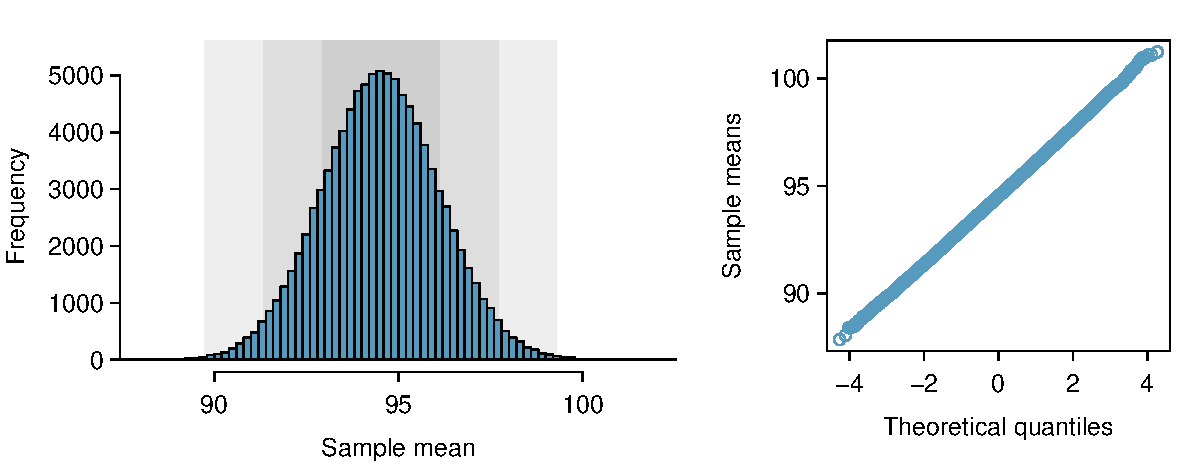
\includegraphics[width=\textwidth]{04-5/figures/netTimeBigSamplingDistribution/netTimeBigSamplingDistribution}
%   \caption{The left panel shows a histogram of the sample means for 100,000 different random samples. The right panel shows a normal probability plot of those sample means.}
%   \label{netTimeBigSamplingDistribution}
%\end{figure}
%
%Does this distribution look familiar? Hopefully so! The distribution of sample means closely resembles the normal distribution (see Section~\ref{normalDist}). A normal probability plot of these sample means is shown in the right panel of Figure~\ref{netTimeBigSamplingDistribution}. Because all of the points closely fall around a straight line, we can conclude the distribution of sample means is nearly normal. This result can be explained by the Central Limit Theorem.
%
%\begin{termBox}{\tBoxTitle{Central Limit Theorem, informal description}
%If a sample consists of at least 30 independent observations and the data are not strongly skewed, then the distribution of the sample mean is well approximated by a~normal model.\index{Central Limit Theorem}}
%\end{termBox}
%
%We will apply this informal version of the Central Limit Theorem for now, and discuss its details further in Section~\ref{cltSection}.
%
%The choice of using 2 standard errors in Equation~(\ref{95PercentConfidenceIntervalFormula}) was based on our general guideline that roughly 95\% of the time, observations are within two standard deviations of the mean. Under the normal model, we can make this more accurate by using 1.96 in place~of~2.
%\begin{eqnarray}
%\text{point estimate}\ \pm\ 1.96\times SE
%\label{95PercentCIWhenUsingNormalModel}
%\end{eqnarray}
%If a point estimate, such as $\bar{x}$, is associated with a normal model and standard error $SE$, then we use this more precise 95\% confidence interval.

A careful eye might have observed the somewhat awkward language used to describe confidence intervals. We reiterate that the correct interpretation is:
%\begin{quote}
``We are $(1-\alpha)$\% confident that the population parameter lies between 
(lower bound of interval) and (upper bound of interval)''.
%\end{quote}
\emph{Incorrect} language might try to describe the confidence interval as capturing the population parameter with a certain probability. 
For example it is wrong to state that we there is a $(1-\alpha)$\% probability that the interval captures the parameter.
This is one of the most common errors: while it might be useful to think of it as a probability, the confidence level only quantifies how plausible it is that the parameter is in the interval.
The term \emph{probability} refers to random events in which outcomes can be different when
an experiment is repeated.
The upper bound and lower bound of a confidence interval are fixed once they have been calculated.
They are not random.
As mentioned earlier in Section~\ref{variabilityInEstimates} the population parameter of interest is also fixed.
Either the parameter is inside the calculated interval or it isn't and there is no randomness involved; 
hence we can not interpret a confidence interval in terms of probability.

Another especially important consideration of confidence intervals is that they \emph{only try to capture the population parameter}. Our intervals say nothing about the confidence of capturing individual observations, a proportion of the observations, or about capturing point estimates. Confidence intervals only attempt to capture population parameters.

\index{confidence interval!interpretation|)}
\index{confidence interval|)}





\subsection{Finding values from the relevant reference distribution}
\label{sectionFindingValuesFromTheRelevantRefDistrib}

%Suppose we want to consider confidence intervals where the confidence level is somewhat higher than 95\%: perhaps we would like a confidence level of 99\%. Think back to the analogy about trying to catch a fish: if we want to be more sure that we will catch the fish, we should use a wider net. To create a 99\% confidence level, we must also widen our 95\% interval. On the other hand, if we want an interval with lower confidence, such as 90\%, we could make our original 95\% interval slightly slimmer.

When we create a confidence interval we attach a certain amount of confidence to it.
The amount of confidence we associate with it depends on a value taken from a reference distribution
as mentioned in Section~\ref{sectionConstructingAnApproximateCConfidenceInterval}.
The reference distribution we use depends on the information provided.
Certain schools of thought like to make the distinction between small and large samples but we will not be doing so.
We will keep things simple (as well as more faithful to the theory).


\begin{termBox}{\tBoxTitle{Summary of reference distributions to use for constructing confidence intervals}

\begin{tabular}{l c l}
When $\sigma$ is known		&	$\longrightarrow$	&	Use the Z distribution	\\
When $\sigma$ is not known	&	$\longrightarrow$	&	Use the $t$ distribution		\\
For proportions				&	$\longrightarrow$	&	Use the Z distribution
\end{tabular}
}
\end{termBox}


\subsubsection{When $\sigma$ is known and for proportions}
\label{sectionCIWhenSigmaKnown}

%The 95\% confidence interval structure provides guidance in how to make intervals with new confidence levels. Below is a general 95\% confidence interval for a point estimate that comes from a nearly normal distribution:
%\begin{eqnarray}
%\text{point estimate}\ \pm\ 1.96\times SE
%\end{eqnarray}
%There are three components to this interval: the point estimate, ``1.96'', and the standard error. The choice of $1.96\times SE$ was based on capturing 95\% of the data since the estimate is within 1.96 standard deviations of the parameter about 95\% of the time. The choice of 1.96 corresponds to a 95\% confidence level. 

When $\sigma$ is known our reference distribution will be the standard normal distribution.
Recall that the letter Z is associated with the standard normal distribution.
The value from standard normal distribution that we require for constructing our confidence interval
is labelled $z_{\alpha/2}$.
The subscript $\frac{\alpha}{2}$ refers to a tail probability in our reference distribution which represents the most extreme cases. 
When we want to construct a $(1 - \alpha)$\% confidence interval, we can calculate $\alpha/2$ to 
determine the tail probabilities of the standard normal distribution and then figure out the value
of $z_{\alpha/2}$ that corresponds to these extreme probabilities.
The area between $-z_{\alpha/2}$ and $+z_{\alpha/2}$ will correspond to a probability of $(1-\alpha)$\%.
Figure~\ref{choosingZForCIGenCase} illustrates this procedure.

\vspace{-1.00cm}
\begin{figure}[H]
\centering
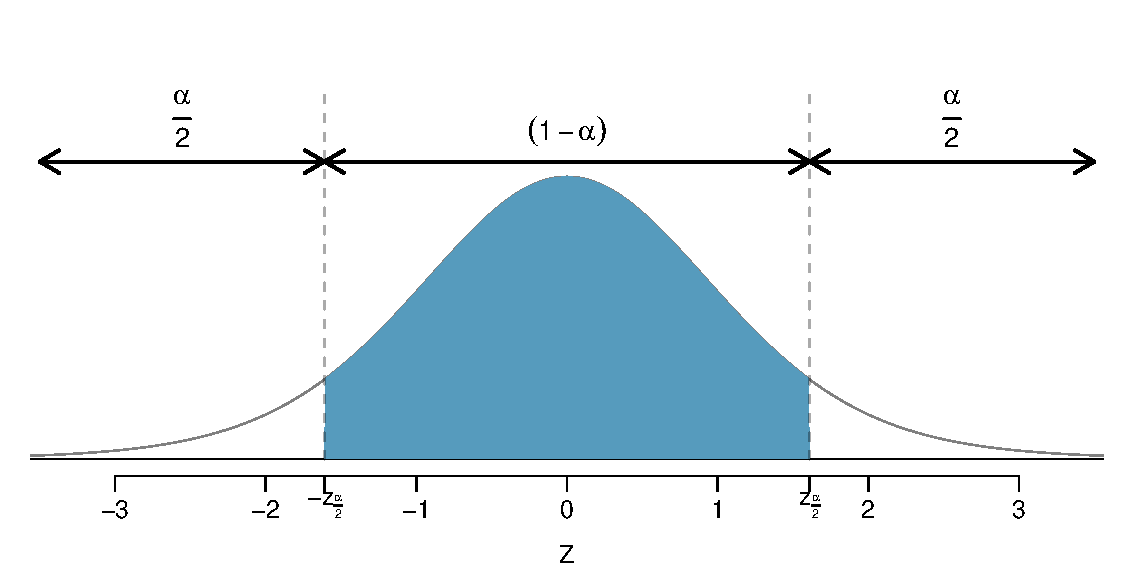
\includegraphics[width=\textwidth]{04-5/figures2/choosingZForCIGeneral/choosingZForCIGeneral.pdf}
\caption{The area between $-z_{\alpha/2}$ and $+z_{\alpha/2}$ corresponds to a $(1-\alpha)$\% confidence interval on a proportion or on the mean when $\sigma$ is known}
\label{choosingZForCIGenCase}
\end{figure}

Let's do several examples with real values.

\begin{example}{Find $z_{\alpha/2}$ for a a 95\% confidence interval when $\sigma$ is known or for proportions.} \label{exampleZalpha95CI} 
This means that we have
\begin{align}
1 - \alpha 		& = 0.95	\\
\frac{\alpha}{2}	& = 0.025
\end{align}
This means that the area in each tail is 0.025.
From Appendix~\ref{distributionTables} we see that this corresponds to a value of $z = 1.96$.
Hence $z_{\alpha/2 = 1.96}$ for a 95\% confidence interval when $\sigma is known$ or on proportions.
This is illustrated in Figure~\ref{choosingZFor95CI}.
\begin{figure}[H]
\centering
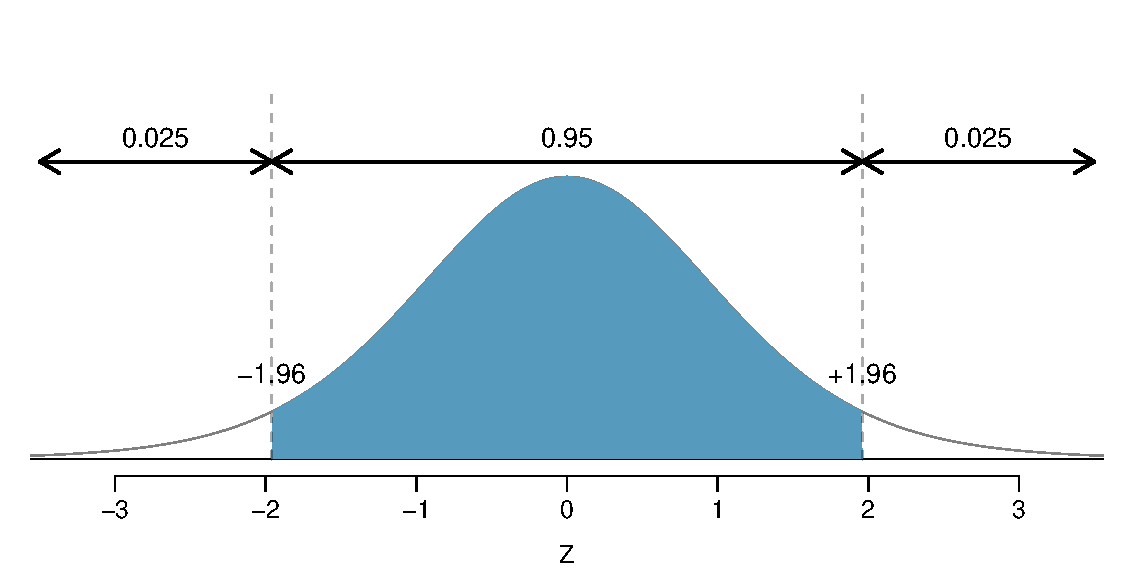
\includegraphics[width=\textwidth]{04-5/figures2/choosingZFor95CI/choosingZFor95CI.pdf}
\caption{The area between $-z_{\alpha/2}=-1.96$ and $+z_{\alpha/2}=+1.96$ corresponds to a 
95\% confidence interval on a proportion or on the mean when $\sigma$ is known}
\label{choosingZFor95CI}
\end{figure}
\end{example}



\begin{example}{Find $z_{\alpha/2}$ for a a 99\% confidence interval when $\sigma$ is known or for proportions.} \label{exampleZalpha99CI} 
We are essentially repeating the procedure in Example~\ref{exampleZalpha95CI} for a 99\% confidence interval when $\sigma$ is known or for proportions.
This time we have
\begin{align}
1 - \alpha 		& = 0.99	\\
\frac{\alpha}{2}	& = 0.005
\end{align}

Now the area we look for in each tail is 0.025.
From Appendix~\ref{distributionTables} we see that this corresponds to a value of $z = 2.58$.
Hence $z_{\alpha/2 = 2.58}$ for a 99\% confidence interval on proportions or when $\sigma$ is known.
This is illustrated in Figure~\ref{choosingZFor99CI}.

\begin{figure}[H]
\centering
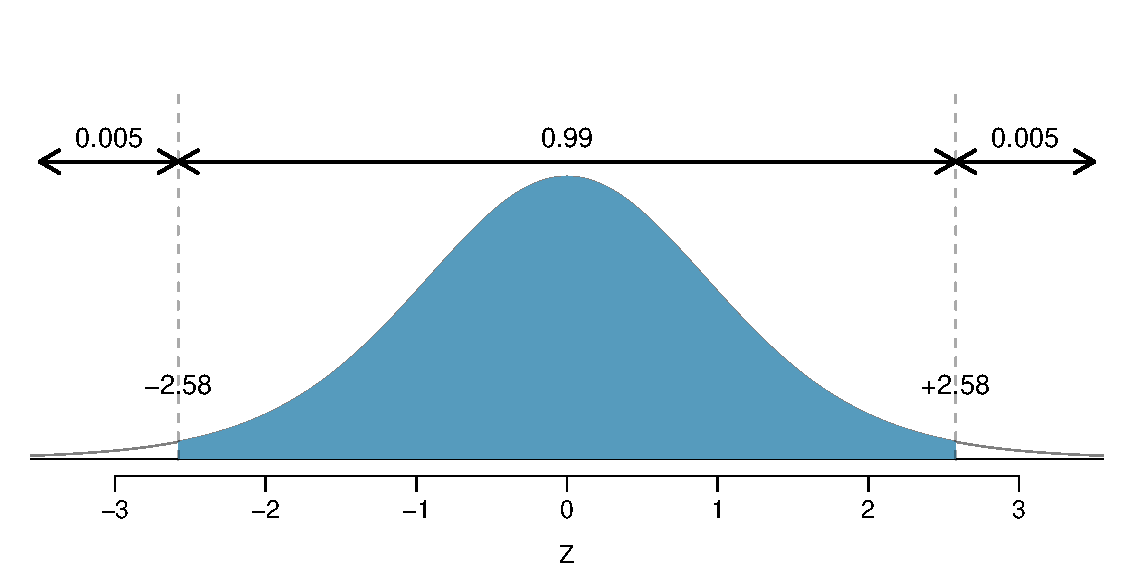
\includegraphics[width=\textwidth]{04-5/figures2/choosingZFor99CI/choosingZFor99CI.pdf}
\caption{The area between $-z_{\alpha/2}=-2.58$ and $+z_{\alpha/2}=+2.58$ corresponds to a 
99\% confidence interval on a proportion or on the mean when $\sigma$ is known}
\label{choosingZFor99CI}
\end{figure}
\end{example}



%To create a 99\% confidence interval, change 1.96 in the 95\% confidence interval formula to be $2.58$. 

%Exercise~\ref{leadInForMakingA99PercentCIExercise} highlights that 99\% of the time a normal random variable will be within 2.58 standard deviations of the mean. This approach -- using the Z scores in the normal model to compute confidence levels -- is appropriate when $\bar{x}$ is associated with a normal distribution with mean $\mu$ and standard deviation $SE_{\bar{x}}$. Thus, the formula for a 99\% confidence interval is
%\begin{eqnarray}
%\bar{x}\ \pm\ 2.58\times SE_{\bar{x}}
%\label{99PercCIForMean}
%\end{eqnarray}

In Figure~\ref{choosingZForCI} we give a comparison of the two different levels of confidence 
(i.e. 95\% and 99\%).
Notice as our level of confidence increases, the value of $|z_{\alpha/2}|$ also increases.

\begin{figure}[H]
\centering
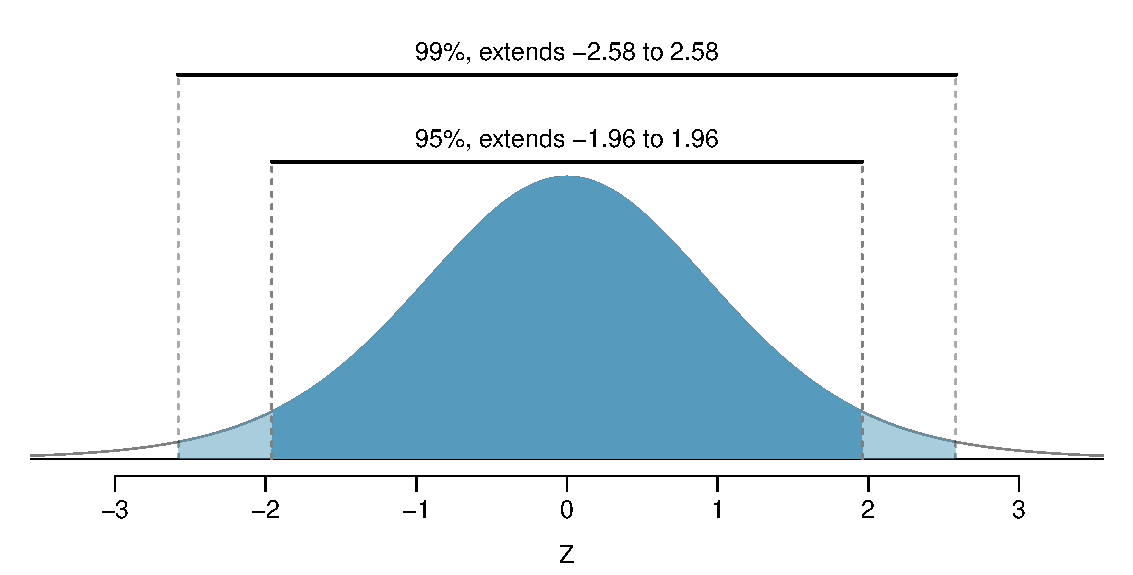
\includegraphics[width=\textwidth]{04-5/figures/choosingZForCI/choosingZForCI}
%\caption{The area between -$z^{\star}$ and $z^{\star}$ increases as $|z^{\star}|$ becomes larger. If the confidence level is 99\%, we choose $z^{\star}$ such that 99\% of the normal curve is between -$z^{\star}$ and $z^{\star}$, which corresponds to 0.5\% in the lower tail and 0.5\% in the upper tail: $z^{\star}=2.58$.}
\caption{The area between $-z_{\alpha/2}$ and $+z_{\alpha/2}$ increases as $|z_{\alpha/2}|$ becomes larger. If the confidence level is 99\%, we choose $z^{\alpha/2}$ such that 99\% of the normal curve is between -$z_{\alpha/2}$ and $+z_{\alpha/2}$, which corresponds to 0.5\% in the lower tail and 0.5\% in the upper tail: $z_{\alpha/2}=2.58$.}
\label{choosingZForCI}
\index{confidence interval!confidence level|)}
\end{figure}


%\begin{exercise} \label{leadInForMakingA99PercentCIExercise}
%If $X$ is a normally distributed random variable, how often will $X$ be within 2.58 standard deviations of the mean?\footnote{This is equivalent to asking how often the $Z$ score will be larger than -2.58 but less than 2.58. (For a picture, see Figure~\ref{choosingZForCI}.) To determine this probability, look up -2.58 and 2.58 in the normal probability table (0.0049 and 0.9951). Thus, there is a $0.9951-0.0049 \approx 0.99$ probability that the unobserved random variable $X$ will be within 2.58 standard deviations of $\mu$.}
%\end{exercise}












\section{One sample confidence intervals}
\label{sectionOneSampleConfidenceIntervals}

\subsection{On the mean}

\subsubsection{When $\sigma$ is known}
\label{sectionCIWhenSigmaIsKnown}

In the case that we know the population standard deviation, the formula for evaluating a
confidence interval is 

\begin{termBox}{\tBoxTitle{A $(100 - \alpha)$\% confidence interval on $\mu$ when $\sigma$ is known}
\begin{equation}
\bar{x}	~~ \pm ~~		z_{\alpha / 2}  \bigg( \frac{\sigma}{ \sqrt{n} } \bigg)\label{eqnCISigmaKnown}\\
%\bar{x}	~~ \pm ~~		z_{ \frac{\alpha}{2} }  \bigg( \frac{\sigma}{ \sqrt{n} } \bigg)
\end{equation}
}
\end{termBox}


%The value of $(1 - \alpha)\%$ is what we called $(1-\alpha)$ in 
%Section~\ref{sectionIntroductionOnCofidenceIntervals} and it is just a number.
%This notation might appear strange right now but it will make more sense in the 
%{\color{red}{chapter on hypothesis testing}}.
The value of $z_{\alpha/2}$ is obtained from the standard normal tables.
To find $z_{\alpha/2}$ we look at the tail probabilities of our reference distribution to determine certain cut off values.
The manner in which we determine the value of $z_{\alpha / 2}$ was
discussed in Chapter~\ref{sectionFindingValuesFromTheRelevantRefDistrib}.
The standard error in Equation~\ref{eqnCISigmaKnown} is $\frac{\sigma}{\sqrt{n}}$
and the margin of error is $z_{\alpha/2} \big( \frac{\sigma}{\sqrt{n}} \big)$.



\begin{example}{Recall the Cherry 2012 Cherry Blossom Run example in the case study in 
Section~\ref{sectionCaseStudyChellyBlosson10MileRun}. \label{exampleCherryBlossom95CI}
If the sample mean times of the 100 sample points from \data{run10Samp} is 95.61 minutes and the standard  deviation of all the runners is 1.58 minutes, what would be an approximate 95\% confidence interval for the average 10 mile time of all runners in the race?
Explicitly state the standard error of the estimate, the margin of error and the 95\% confidence interval}
We have $n=100$, $\bar{x} = 95.61$ and $\sigma = 1.58$.
The standard error calculated using the standard deviation is 
\begin{align*}
SE	=	\frac{15.78}{\sqrt{100}} & = 1.58
\end{align*}
%which is how we usually proceed since the population standard deviation is generally unknown.
From Example~\ref{exampleZalpha95CI} we know that the value of $z_{\alpha/2} = 1.96$.
%We apply Equation~(\ref{95PercentConfidenceIntervalFormula}):
Therefore the margin of error is
\begin{align*}
MOE	=	1.96 \times \frac{15.78}{\sqrt{100}} & = 3.10
\end{align*}

We apply Equation~(\ref{eqnCISigmaKnown}) to get the entire confidence interval:
%\begin{eqnarray*}
%95.61\ \pm\ 1.96 \times  1.58 \quad \rightarrow \quad (92.45, 98.77)
%\end{eqnarray*}
\begin{eqnarray*}
%95.61\ \pm\ 1.96 \times  1.58 \quad \rightarrow \quad (92.51, 98.71)
95.61\ \pm\ 3.10 =  (92.51, 98.71)
\end{eqnarray*}
Based on these data, we are about 95\% confident that the average 10 mile time for all runners in the race was larger than 92.45 but less than 98.77 minutes. Our interval extends out 2 standard errors from the point estimate, $\bar{x}$.
\end{example}
% library(openintro); library(xtable); data(run10); data(run10Samp); mean(run10Samp$time); sd(run10Samp$time); sd(run10$time, na.rm=TRUE)


\begin{example}{Give an interpretation of the confidence interval created in Example~\ref{exampleCherryBlossom95CI}}
In Example~\ref{exampleCherryBlossom95CI} we constructed a 95\% confidence interval
for the true mean time taken for the 10 mile run.
Therefore the interpretation is that we are 95\% confident that the true mean time for all runners 
to complete the 10 mile Cherry Blossom Run in 2012 is between 92.51 minutes and 98.71 minutes.
\end{example}

\begin{exercise} \label{95CIExerciseForAgeOfRun10Samp1}
The sample data suggest the average runner's age is about 35.05 years with a standard error of 0.90 years (estimated using the sample standard deviation, 8.97). What is an approximate 95\% confidence interval for the average age of all of the runners?\footnote{Again apply Equation~(\ref{95PercentConfidenceIntervalFormula}): $35.05 \ \pm \ 2\times 0.90 \rightarrow (33.25, 36.85)$. We interpret this interval as follows: We are about 95\% confident the average age of all participants in the 2012 Cherry Blossom Run was between 33.25 and 36.85 years.}
\end{exercise}
%library(openintro); data(run10Samp); mean(run10Samp$age); sd(run10Samp$age)


\begin{exercise} \label{find99CIForRun10AgeExercise}
Create a 99\% confidence interval for the average age of all runners in the 2012 Cherry Blossom Run. The point estimate is $\bar{y} = 35.05$ and the standard error is $SE_{\bar{y}} = 0.90$.\footnote{The observations are independent 
%(simple random sample, $<10\%$ of the population), the sample size is at least 30 ($n=100$), and the distribution is only slightly skewed (Figure~\ref{run10SampHistograms}); the normal approximation and estimate of SE should be reasonable. 
with $n=100$.
Apply the 99\% confidence interval formula: $\bar{y}\ \pm\ 2.58 \times  SE_{\bar{y}} = (32.7, 37.4)$. We are 99\% confident that the average age of all runners is between 32.7 and 37.4 years.}
\end{exercise}
%library(openintro); data(run10Samp); d <- run10Samp; mean(d$age); sd(d$age)/sqrt(100)



Table~\ref{tableCommonValuesOfZAlpha} gives some common values of 
$z_{\alpha/2}$ along with their corresponding level of confidence.

\begin{table}[H]
\centering
\begin{tabular}{c | c}
\hline
Level of 		& $z_{\alpha/2}$	\\
Confidence	&				\\
\hline
80			&	1.28		\\
90			&	1.65		\\
95			&	1.96		\\
99			&	2.58		\\
\hline
\end{tabular}
\caption{Values of $z_{\alpha/2}$ that are commonly used along with their corresponding level of confidence.}
\label{tableCommonValuesOfZAlpha}
\end{table}

Table~\ref{tableCommonValuesOfZAlpha} is provided mainly for convenience.
It is best to be able to find the value of $z_{\alpha/2}$ for any level of confidence
rather than to memorize the numbers in this table.
Statistics is about understanding and applying concepts rather than memorizing.


\begin{exercise} \label{find90CIForRun10AgeExercise}
Use the data in Exercise~\ref{find99CIForRun10AgeExercise} to create a 90\% confidence interval for the average age of all runners in the 2012 Cherry Blossom Run.\footnote{We first find $z^{\star}$ such that 90\% of the distribution falls between -$z^{\star}$ and $z^{\star}$ in the standard normal model, $N(\mu=0, \sigma=1)$. We can look up -$z^{\star}$ in the normal probability table by looking for a lower tail of 5\% (the other 5\% is in the upper tail), thus $z^{\star}=1.65$. The 90\% confidence interval can then be computed as $\bar{y}\ \pm\ 1.65\times SE_{\bar{y}} \to (33.6, 36.5)$. (We had already verified conditions for normality and the standard error.) That is, we are 90\% confident the average age is larger than 33.6 but less than 36.5 years.}
\end{exercise}



In reality there are very few situations when $\sigma$ is known and the confidence interval we create for the mean is usually
the one in section~\ref{sectionsectionCIWhenSigmaIsNOTKnown} when $\sigma$ is unknown.
However there are rare instances when we can use Equation~(\ref{eqnCISigmaKnown})
and we explored this confidence interval since we can see how the elements in Chapter~\ref{sectionBasicFoundationsForInference} come together in creating a confidence interval.
The confidence interval created when $\sigma$ is known is also the 
simplest confidence interval on the mean and it is a good idea to start with something basic before moving
on to more advanced situations.


\hfill\\
{\color{red}{FILL UP WITH SOMETHING}}

\vfill


\pagebreak

\subsubsection{When $\sigma$ is not known}
\label{sectionsectionCIWhenSigmaIsNOTKnown}
\label{oneSampleTConfidenceIntervals}

In the case that we know the population standard deviation is not known, the formula for evaluating a
confidence interval is 

\begin{termBox}{\tBoxTitle{A $(100 - \alpha)$\% confidence interval on $\mu$ when $\sigma$ is not known}
\begin{equation}
\bar{x}	~~ \pm ~~		t_{(\alpha / 2, \, n-1)}  \bigg( \frac{ s }{ \sqrt{n} } \bigg)\label{eqnCISigmaNOTKnown}	\\
%\bar{x}	~~ \pm ~~		z_{ \frac{\alpha}{2} }  \bigg( \frac{\sigma}{ \sqrt{n} } \bigg)
\end{equation}
}
\end{termBox}

Notice the similarity between Equation~(\ref{eqnCISigmaNOTKnown}) and Equation~(\ref{eqnCISigmaKnown}).
When $\sigma$ is not known we use the sample standard deviation $s$ instead and
we use a value from $t$ distribution from Chapter~\ref{introducingTheTDistribution} instead of
a value from the standard normal distribution.
The value $t_{(\alpha / 2, n-1)}$ has two subscripts.
The subscript of $\frac{\alpha}{2}$ refers to the tail value of the $t$ distribution that we 
are interested in and the subscript of $(n-1)$ are the degrees of freedom.
This was mentioned briefly in Section~\ref{sectiontTable}
and in particular 
the manner in which we read the $t$ table was discussed in Chapter~\ref{sectiontTable}.
The standard error of the mean in $\ref{eqnCISigmaNOTKnown}$
is $\big( \frac{ s }{ \sqrt{n} } \big)$
and the margin of error is
$t_{(\alpha / 2, \, n-1)}  \big( \frac{ s }{ \sqrt{n} } \big)$.



\begin{termBox}{\tBoxTitle{Degrees of freedom for a single sample}
If the sample has $n$ observations and we are examining a single mean, then we use the $t$ distribution with $df=n-1$ degrees of freedom.}
\end{termBox}



Since $\sigma$ is not known we loose information from our sample.
This is the reason that we use the $t$ distribution instead of the standard since
the extra thick tails of the $t$ distribution are exactly the correction we need to resolve the problem of a poorly estimated standard error.
An intuitive explanation to the reason
we use $n-1$ degrees of freedom instead of $n$ is because we are using $s$ instead of $\sigma$.
This means we are loosing 1 piece of information.


%???? EXPLAIN WHY n-1 DF ???
%???? EXPLAIN WHY n-1 DF ???
%???? EXPLAIN WHY n-1 DF ???
%???? EXPLAIN WHY n-1 DF ???
%???? EXPLAIN WHY n-1 DF ???

%from the $t$ distribution at $n-1$ degrees of freedom.

%\subsection{One sample $t$ confidence intervals}


\begin{figure}[H]
\centering
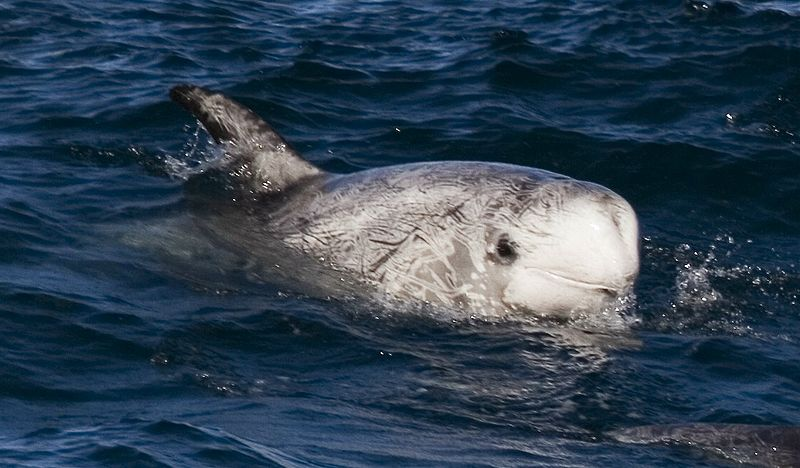
\includegraphics[width=0.70\textwidth]{05/figures/rissosDolphin/rissosDolphin.jpg}  \\
\addvspace{2mm}
\begin{minipage}{\textwidth}
   \caption[rissosDolphinPic]{A Risso's dolphin.\vspace{-1mm} \\
   -----------------------------\vspace{-2mm}\\
   {\footnotesize Photo by Mike Baird (\urlwofont{http://www.bairdphotos.com/}).%Image is under Creative Commons Attribution 2.0 Generic.
}\vspace{-8mm}}
   \label{rissosDolphin}
\end{minipage}
\vspace{3mm}
\end{figure}
\setlength{\captionwidth}{\mycaptionwidth}

Let's explore this type of confidence interval with a real world example involving marine life.
Dolphins are at the top of the oceanic food chain, which causes dangerous substances such as mercury to concentrate in their organs and muscles. This is an important problem for both dolphins and other animals, like humans, who occasionally eat them. For instance, this is particularly relevant in Japan where school meals have included dolphin at times.
\setlength{\captionwidth}{71.5mm}

Here we identify a confidence interval for the average mercury content in dolphin muscle using a sample of 19 Risso's dolphins from the Taiji area in Japan.\footnote{Taiji was featured in the movie \emph{The Cove}, and it is a significant source of dolphin and whale meat in Japan. Thousands of dolphins pass through the Taiji area annually, and we will assume these 19 dolphins represent a simple random sample from those dolphins. Data reference: Endo T and Haraguchi K. 2009. High mercury levels in hair samples from residents of Taiji, a Japanese whaling town. Marine Pollution Bulletin 60(5):743-747.} The data are summarized in Table~\ref{summaryStatsOfHgInMuscleOfRissosDolphins}. The minimum and maximum observed values can be used to evaluate whether or not there are obvious outliers or skew.

\begin{table}[H]
\centering
\begin{tabular}{ccc cc}
\hline
$n$ & $\bar{x}$ & $s$ & minimum & maximum \\
19   & 4.4	  & 2.3  & 1.7	       & 9.2 \\
\hline
\end{tabular}
\caption{Summary of mercury content in the muscle of 19 Risso's dolphins from the Taiji area. Measurements are in $\mu$g/wet g (micrograms of mercury per wet gram of muscle).}
\label{summaryStatsOfHgInMuscleOfRissosDolphins}
\end{table}

%\begin{example}{Are the independence and normality conditions satisfied for this data~set?}
%The observations are a simple random sample and consist of less than 10\% of the population, therefore independence is reasonable. The summary statistics in Table~\ref{summaryStatsOfHgInMuscleOfRissosDolphins} do not suggest any skew or outliers; all observations are within 2.5 standard deviations of the mean. Based on this evidence, the normality assuagemption seems reasonable.
%\end{example}

%In the normal model, we used $z^{\star}$ and the standard error to determine the width of a confidence interval. We revise the confidence interval formula slightly when using the $t$ distribution:
%\begin{eqnarray*}
%\bar{x} \ \pm\  t^{\star}_{df}SE
%\end{eqnarray*}
%\marginpar[\raggedright\vspace{-9mm}
%
%$t^{\star}_{df}$\vspace{1mm}\\\footnotesize Multiplication\\factor for\\$t$ conf. interval]{\raggedright\vspace{-9mm}

%$t^{\star}_{df}$\vspace{1mm}\\\footnotesize Multiplication\\factor for\\$t$ conf. interval}
The sample mean and estimated standard error are computed just as before ($\bar{x} = 4.4$ and $SE = s/\sqrt{n} = 0.528$). The value $t_{(\alpha/2, \, n-1)}$ is a cutoff we obtain based on the confidence level and the $t$ distribution with $df$ degrees of freedom. Before determining this cutoff, we will first need the degrees of freedom.


In our current example, we should use the $t$ distribution with $df=19-1=18$ degrees of freedom. Then identifying $t_{(\alpha/2, 18)}$ is similar to how we found $z_{\alpha/2}$.
\begin{itemize}
\setlength{\itemsep}{0mm}
\item For a 95\% confidence interval, we want to find the cutoff $t_{(\alpha/2, 18)}$ such that 95\% of the $t$ distribution is between -$t_{(\alpha/2, 18)}$ and $t_{(\alpha/2, 18)}$.
This means we are interested in $t_{(0.025, 18)}$.
\item We look in the $t$ table on page~\pageref{tTableSample}, find the column with area totalling 0.05 in the two tails (third column), and then the row with 18 degrees of freedom: $t_{(0.025, 18)} = 2.10$.
\end{itemize}
Generally the value of $t_{(\alpha/2, n-1)}$ is slightly larger than what we would get under the normal model with~$z_{\alpha/2}$.



Finally, we can substitute all our values into the confidence interval equation to create the 95\% confidence interval for the average mercury content in muscles from Risso's dolphins that pass through the Taiji area:
%\begin{eqnarray*}
%\bar{x} \ \pm\  t^{\star}_{18}SE
%	\quad \to \quad
%4.4 \ \pm\  2.10 \times 0.528
%	\quad \to \quad
%(3.29, 5.51)
%\end{eqnarray*}
\begin{eqnarray*}
4.4 \ \pm\  2.10 \times 0.528	 = 	(3.29, 5.51)
\end{eqnarray*}
We are 95\% confident the average mercury content of muscles in Risso's dolphins is between 3.29 and 5.51 $\mu$g/wet gram. This is above the Japanese regulation level of 0.4 $\mu$g/wet gram.

\index{data!dolphins and mercury|)}

%\begin{termBox}{\tBoxTitle{Finding a $t$ confidence interval for the mean}
%Based on a sample of $n$ independent and nearly normal observations, a confidence interval for the population mean is
%\begin{eqnarray*}
%\bar{x} \ \pm\  t^{\star}_{df}SE
%\end{eqnarray*}
%where $\bar{x}$ is the sample mean, $t^{\star}_{df}$ corresponds to the confidence level and degrees of freedom, and $SE$ is the standard error as estimated by the sample.}
%\end{termBox}

\begin{exercise} \label{croakerWhiteFishPacificExerConditions}
\index{data!white fish and mercury|(}
The FDA's webpage provides some data on mercury content of fish.\footnote{\urlwofont{http://www.fda.gov/food/foodborneillnesscontaminants/metals/ucm115644.htm}} Based on a sample of 15 croaker white fish (Pacific), a sample mean and standard deviation were computed as 0.287 and 0.069 ppm (parts per million), respectively. The 15 observations ranged from 0.18 to 0.41 ppm. We will assume these observations are independent. Based on the summary statistics of the data, do you have any objections to the normality condition of the individual observations?\footnote{There are no obvious outliers; all observations are within 2 standard deviations of the mean. If there is skew, it is not evident. There are no red flags for the normal model based on this (limited) information, and we do not have reason to believe the mercury content is not nearly normal in this type of fish.}
\end{exercise}

\begin{example}{Estimate the standard error of $\bar{x}=0.287$ ppm using the data summaries in Exercise~\ref{croakerWhiteFishPacificExerConditions}. If we are to use the $t$ distribution to create a 90\% confidence interval for the actual mean of the mercury content, identify the degrees of freedom we should use and also find $t_{(\alpha/2, \, n-1)}$.}
\label{croakerWhiteFishPacificExerSEDFTStar}
The standard error is $SE = \frac{0.069}{\sqrt{15}} = 0.0178$. Degrees of freedom: $df = n - 1 = 14$.

Looking in the column where two tails is 0.100 (for a 90\% confidence interval) and row $df=14$, we identify $t_{(\alpha/2, \, n-1)} = t_{(0.05, \,14)} = 1.76$.
\end{example}

\begin{example}{Using the results of Exercise~\ref{croakerWhiteFishPacificExerConditions} and Example~\ref{croakerWhiteFishPacificExerSEDFTStar}, compute a 90\% confidence interval for the average mercury content of croaker white fish (Pacific).}\label{croakerWhiteFishPacificCICalc}
Using data summaries from Exercise~\ref{croakerWhiteFishPacificExerConditions}
and the values obtained in Example~\ref{croakerWhiteFishPacificExerSEDFTStar} we see that
\begin{align}
\bar{x} \ \pm\ t_{0.1, \,14} SE \ =  0.287 \ \pm\  1.76 \times 0.0178\ = \ (0.256, 0.318) 
\end{align}

\end{example}



\begin{example}{provide an interpretation of the confidence interval calculated in Example~\ref{croakerWhiteFishPacificCICalc} }
We are 90\% confident that the average mercury content of croaker white fish (Pacific) is between 0.256 and 0.318 ppm.
\end{example}
\index{data!white fish and mercury|)}


{\color{red}{FILL UP WITH SOMETHING}}

\vfill

\pagebreak

\subsection{On a proportion}

In the case that we are interested constructing a confidence interval for a proportion proportion, 
the formula we use is


\begin{termBox}{\tBoxTitle{A $(100 - \alpha)$\% confidence interval on $p$}
\begin{equation}
\hat{p}	~~ \pm ~~		z_{\alpha / 2} 	\sqrt{ \frac{\hat{p}(1 - \hat{p})}{n} }	\label{eqnCIOnP}\\
%\bar{x}	~~ \pm ~~		z_{ \frac{\alpha}{2} }  \bigg( \frac{\sigma}{ \sqrt{n} } \bigg)
\end{equation}
}
\end{termBox}
\vspace{0.25cm}

In Equation~\ref{eqnCIOnP} $\sqrt{ \frac{\hat{p}(1 - \hat{p})}{n} }$ is the standard error of proportion
and $z_{\alpha / 2} 	\sqrt{ \frac{\hat{p}(1 - \hat{p})}{n} }$ is the margin of error.
Recall that a proportion is a fraction of the overall population.
We use the methods in this chapter to answer questions like the following real life example:
\begin{itemize}
\setlength{\itemsep}{0mm}
\item What proportion of the American public approves of the job the Supreme Court is doing?
\item The Pew Research Center conducted a poll about support for the 2010 health care law, and they used two forms of the survey question. Each respondent was randomly given one of the two questions. What is the difference in the support for respondents under the two question orderings?
\end{itemize}
%We will find that the methods we learned in previous chapters are very useful in these settings. For example, sample proportions are well characterized by a nearly normal distribution when certain conditions are satisfied, making it possible to employ the usual confidence interval and hypothesis testing tools. In other instances, such as those with contingency tables or when sample size conditions are not met, we will use a different distribution, though the core ideas remain the same.


\index{data!supreme court|(}

Let's work out this example.
According to a New York Times / CBS News poll in June 2012, only about 44\% of the American public approves of the job the Supreme Court is doing.\footnote{\href{http://www.nytimes.com/2012/06/08/us/politics/44-percent-of-americans-approve-of-supreme-court-in-new-poll.html}{\scriptsize nytimes.com/2012/06/08/us/politics/44-percent-of-americans-approve-of-supreme-court-in-new-poll.html}} This poll included responses of 976 adults.

A sample proportion can be described as a sample mean (of sorts). If we represent each ``success'' as a 1 and each ``failure'' as a 0, then the sample proportion is the mean of these numerical outcomes:
\begin{eqnarray*}
\hat{p} = \frac{\ 0 + 1 + 1 + s + 0\ }{976} = 0.44
\end{eqnarray*}
The distribution of $\hat{p}$ is nearly normal when the distribution of 0's and 1's is not too strongly skewed for the sample size. The most common guideline for sample size and skew when working with proportions is to ensure that we expect to observe a minimum number of successes and failures, typically at least 10 of each.
Let's now estimate the standard error of $\hat{p}=0.44$ using Equation~\eqref{eqnCIOnP}. 
\begin{align*}
SE = \sqrt{\frac{\hat{p}(1-\hat{p})}{n}} = \sqrt{\frac{0.44(1-0.44)}{976}} = 0.016
\end{align*}

Let's now construct a 95\% confidence interval for $p$, the proportion of Americans who approve of the job the Supreme Court is doing.
From Chapters~\ref{sectionCIWhenSigmaIsKnown} and \ref{sectionFindingValuesFromTheRelevantRefDistrib}
we know that $z_{\alpha/2} = 1.96$ for a 95\% confidence interval.
Therefore the confidence interval may be computed as
\begin{eqnarray*}
0.44 \ \pm\ 1.96\times 0.016 = (0.409, 0.471)
\end{eqnarray*}
We are 95\% confident that the true proportion of Americans who approve of the job of the Supreme Court (in June 2012) is between 0.409 and 0.471. If the proportion has not changed since this poll, than we can say with high confidence that the job approval of the Supreme Court is below 50\%.

\index{data!supreme court|)}





\subsection{Assumptions}

\subsubsection{On the mean}

For confidence intervals on $\mu$ the assumptions that are required are the following

\begin{enumerate}
\item	Data is from a random sample from a large population.
\item	The sample size should be less than 10\% of the population.
\item	Observations in the sample must be independent of each other.
\item	If the sample size is small, the population distribution should be normal or at least approximately normal. \label{assumpNormalPop}
\end{enumerate}

We are mainly concerned on sample size in assumption~\ref{assumpNormalPop} because the effect of the central limit theorem will provide us with a sampling distribution of $\bar{x}$ that is approximately normal for sufficiently large $n$.
When $\sigma$ is not known and we using the $t$ distribution is still valid because the $t$ begins
to resemble the standard normal distribution.



\subsubsection{On a proportion}
\label{sectionAssumpOnProp}

For confidence intervals on $p$ the assumptions that are required are the following

\begin{enumerate}
\item	Data is from a random sample from a large population.
\item	Observations in the sample are independent of each other.
\item	$np \geq 10$ and $n(1-p) \geq 10$ \label{npAssumpForOneSampleProp}
\end{enumerate}

Since $p$ is unknown we can attempt to verify assumption~\ref{npAssumpForOneSampleProp} by 
estimating $p$ with $\hat{p}$ and checking whether $n\hat{p} \geq 10$ and $n(1-\hat{p}) \geq 10$. 


\section{Two sample confidence intervals}
\label{sectionTwoSampleConfidenceIntervals}

\subsection{On a difference of two means}
\label{differenceOfTwoMeans}


In this section we consider a difference in two population means, $\mu_1 - \mu_2$, under the condition that the data are not paired
(i.e. our parameter of interest is $\mu_1 - \mu_2$).
Paired data are discussed in Chapter~\ref{sectionPairedData}.
The methods are similar in theory to those of Chapter~\ref{sectionOneSampleConfidenceIntervals}
but different in the details.
%Just as with a single sample, we identify conditions to ensure a point estimate of the difference $\bar{x}_1 - \bar{x}_2$ is nearly normal. Next we introduce a formula for the standard error, which allows us to apply our general tools from Section~\ref{aFrameworkForInference}.


\subsubsection{When $\sigma_{1}$ and $\sigma_{2}$ are known}

This is the most basic two sample confidence interval on a difference of means.

\begin{termBox}{\tBoxTitle{A $(100 - \alpha)$\% confidence interval on $\mu_{1} - \mu_{2}$ when 
$\sigma_{1}$ and $\sigma_{2}$ are known}
\begin{equation}
\bar{x}_{1} - \bar{x}_{2}	~~ \pm ~~		z_{\alpha / 2}  \sqrt{ \frac{\sigma_1^2}{n_1} + \frac{\sigma_2^2}{n_2} }\label{eqnCIDiffMeanSigmasKnown}
\end{equation}
}
\end{termBox}

In Equation~\eqref{eqnCIDiffMeanSigmasKnown} 
%$\sqrt{ \frac{\sigma_1^2}{n_1} + \frac{\sigma_2^2}{n_2} }$
the term under the square root
is the standard error on the difference of means and
%$z_{\alpha / 2}  \sqrt{ \frac{\sigma_1^2}{n_1} + \frac{\sigma_2^2}{n_2} }$ 
this term multiplied by $z_{\alpha/2}$
is the margin of error.
There are very few cases where Equation~\eqref{eqnCIDiffMeanSigmasKnown} is used
since it is very rare to know the standard deviations of two populations.




\subsubsection{When $\sigma_{1}$ and $\sigma_{2}$ are not known}

When are interested in the difference of means of two populations and the
standard deviations of both populations are not known we have to consider two possibilities.
They are when $\sigma_{1} \neq \sigma_{2}$ or when $\sigma_{1} = \sigma_{2}$.
%There are tests for equality of variance that can be performed but those are more suited for more advanced texts in statistics.
%
%We break down this section into 2 cases which are when the standard deviations of both populations
%are known and when they are both unknown.
The case in which the standard deviations are both not known are broken down into 2 further
sub-cases in which the standard deviations are known to be (or at least assumed) equal or not equal.
Since this is an introductory text in statistics, we may consider that we either know or at least we can assume 
$\sigma_{1} \neq \sigma_{2}$ or $\sigma_{1} = \sigma_{2}$ based on 
additional information available from the study or expert knowledge in the area of interest.
Typically when there is knowledge of equal population standard deviations,
we usually observe sample standard deviations that are also relatively close.

\begin{termBox}{\tBoxTitle{Caution about assuming equal standard deviations}
In general do not assume $\sigma_{1} = \sigma_{2}$.
}
\end{termBox}

If we do not have any information about equal or unequal population standard deviations we should
not make assumptions about them.
There is a \emph{crude rule of thumb} that can be applied which is that if
If the larger sample standard deviation divided by the smaller sample standard 
deviation is greater or equal to two then we should not assume $\sigma_{1} = \sigma_{2}$.
By this we mean that if
\begin{equation*}
\frac{ \max(s_{1}, \, s_{2}) }{ \min(s_{1}, \, s_{2}) } \geq 2 \quad \to \quad \text{do not assume $\sigma_{1} = \sigma_{2}$}
\end{equation*}
This rule of thumb states that if our sample standard deviations are different enough we can not safely 
assume $\sigma_{1} = \sigma_{2}$.
%We reiterate however that there are statistical tests available to assess the equality of variance assumption.
There are statistical tests available to assess the assumption of equality of variance however such tests are more suited for more advanced texts in statistics.



\paragraph{When $\sigma_{1} \neq \sigma_{2}$}


\begin{termBox}{\tBoxTitle{A $(100 - \alpha)$\% confidence interval on $\mu_{1} - \mu_{2}$ when 
$\sigma_{1}$ and $\sigma_{2}$ are not known and $\sigma_{1} \neq \sigma_{2}$}
%The sample difference of two means, $\bar{x}_1 - \bar{x}_2$, is nearly normal with mean $\mu_{1}-\mu_{2}$ and estimated standard error
%%\begin{eqnarray}
%%\textstyle
%%SE_{\bar{x}_{1} - \bar{x}_{2}} = \sqrt{\frac{s_1^2}{n_1} + \frac{s_2^2}{n_2}}
%%\label{seOfDifferenceInMeans}
%%\end{eqnarray}
\begin{equation}
\bar{x}_{1} - \bar{x}_{2}	~~ \pm ~~		t_{(\alpha / 2, \, d)}  \sqrt{ \frac{s_1^2}{n_1} + \frac{s_2^2}{n_2} }\label{eqnCIDiffMeanSigmasNotKnownAndDifferent}
\end{equation}
where a conservative estimate of $d$ is
\begin{equation}
d = \min(n_1 - 1, \, n_2 - 1)
\end{equation}
%%\bar{x}	~~ \pm ~~		z_{ \frac{\alpha}{2} }  \bigg( \frac{\sigma}{ \sqrt{n} } \bigg)
}
\end{termBox}

Note that we stated that $d$ is a conservative estimate of the degrees of freedom.
A more accurate value of $d$ is given by 

\begin{equation}
d = \frac{ \bigg( \displaystyle \frac{ s_{1}^{2} }{ x_{1} } + \frac{ s_{2}^{2} }{ x_{2} } \bigg)^{2} }{ \displaystyle \frac{ ( s_{1}^{2} / n_{1} )^{2} }{ n_{1} - 1 }	+	\frac{ ( s_{2}^{2} / n_{2} )^{2} }{ n_{2} - 1 } }\label{eqnAccurateDF}
\end{equation}

The value calculated be Equation~\eqref{eqnAccurateDF} is typically a real number and not 
an integer and this is perfectly fine (Recall Chapter~\ref{introducingTheTDistribution}).
We can either be conservative and take the floor\footnote{The floor refers to rounding down to the nearest integer.}
 of the value calculated in Equation~\eqref{eqnAccurateDF}
or we can use software to obtain a more accurate value.


%\begin{caution}
%{Independence for random processes and experiments}
%{If a sample is from a random process or experiment, it is important to verify the observations from the process or subjects in the experiment are nearly independent and maintain their independence throughout the process or experiment. Usually subjects are considered independent if they undergo random assignment in an experiment.}
%\end{caution}



\begin{caution}
{Welch's Interval and the Behrens---Fisher problem}
{This method outlined in Equation~\ref{eqnCIDiffMeanSigmasNotKnownAndDifferent}
is known as \term{WelchÕs Interval} and it is a good approximation for the situation in this chapter.
In reality interval estimation (as well as hypothesis testing) on a difference of two means from two independent samples from two normally distributed populations when $\sigma_{1} \neq \sigma{2}$ is an open problem called the \term{BehrensFisher problem}. }
\end{caution}



%%\subsection{Confidence interval for the difference}
%
%%We apply these methods to two examples: participants in the 2012 Cherry Blossom Run and newborn infants. This section is motivated by questions like ``Is there convincing evidence that newborns from mothers who smoke have a different average birth weight than newborns from mothers who don't smoke?''
%
%\index{data!run10Samp|(}
%
%We will apply Equation~\eqref{eqnCIDiffMeanSigmasNotKnownAndDifferent} 
%to construct a 95\% confidence interval on a difference of means to the participants in the 2012 Cherry Blossom Run from the case study in Chapter~\ref{sectionCaseStudyChellyBlosson10MileRun}.
%We would like to estimate the average difference in run times for men and women using the \data{run10Samp} data set, which was a simple random sample of 45 men and 55 women from all runners in the 2012 Cherry Blossom Run. Table~\ref{cherryBlossomRun2009SampleOf180SummaryStats} presents relevant summary statistics, and box plots of each sample are shown in Figure~\ref{cbrRunTimesMenWomen}.
%
%\begin{table}[H]
%\centering
%\begin{tabular}{l rr}
%\hline
%	&	men	&	women \\
%\hline
%$\bar{x}$	& 87.65	& 102.13 \\
%$s$	&	12.5		& 15.2 \\
%$n$	&	45		& 55    \\
%\hline
%\end{tabular}
%\caption{Summary statistics for the run time of 100 participants in the 2009 Cherry Blossom Run.}
%\label{cherryBlossomRun2009SampleOf180SummaryStats}
%\end{table}
%%library(openintro); data(run10Samp); d <- run10Samp; by(d$time, d$gender, mean); by(d$time, d$gender, sd); by(d$time, d$gender, length)
%
%\begin{figure}[H]
%\centering
%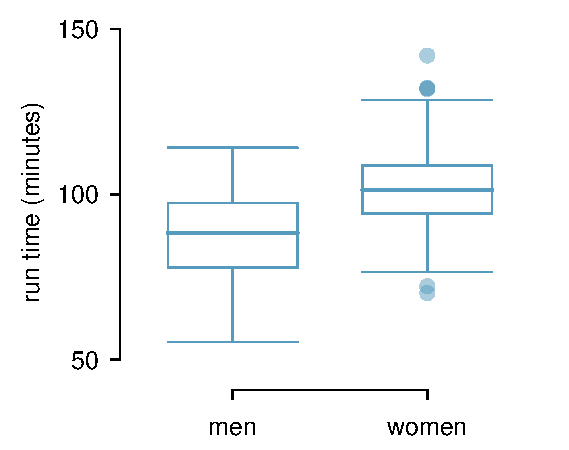
\includegraphics[width=0.5\textwidth]{05/figures/cbrRunTimesMenWomen/cbrRunTimesMenWomen}
%\caption{Side-by-side box plots for the sample of 2009 Cherry Blossom Run participants.}
%\label{cbrRunTimesMenWomen}
%\end{figure}
%
%The two samples are independent of one-another, so the data are not paired. Instead a point estimate of the difference in average 10 mile times for men and women, $\mu_w - \mu_m$, can be found using the two sample means:
%\begin{eqnarray*}
%\bar{x}_{w} - \bar{x}_{m}\ =\ 102.13 - 87.65\ =\ 14.48
%\end{eqnarray*}
%%Because we are examining two simple random samples from less than 10\% of the population, each sample contains at least 30 observations, and neither distribution is strongly skewed, we can safely conclude the sampling distribution of each sample mean is nearly normal. Finally, because each sample is independent of the other (e.g. the data are not paired), we can conclude that the difference in sample means can be modeled using a normal distribution.\footnote{Probability theory guarantees that the difference of two independent normal random variables is also normal. Because each sample mean is nearly normal and observations in the samples are independent, we are assured the difference is also nearly normal.}
%
%%\begin{termBox}{\tBoxTitle{Conditions for normality of $\bar{x}_1 - \bar{x}_2$}
%%If the sample means, $\bar{x}_1$ and $\bar{x}_2$, each meet the criteria for having nearly normal sampling distributions and the observations in the two samples are independent, then the difference in sample means, $\bar{x}_1 - \bar{x}_2$, will have a sampling distribution that is nearly normal.}
%%\end{termBox}
%
%We can quantify the variability in the point estimate, $\bar{x}_{w} - \bar{x}_{m}$, using the following formula for its standard error:
%\index{standard error!difference in means}
%%\begin{eqnarray*}
%%%SE_{\bar{x}_{w} - \bar{x}_{m}} = \sqrt{\frac{\sigma_{w}^2}{n_{w}} + \frac{\sigma_{m}^2}{n_{m}}}
%%SE_{\bar{x}_{w} - \bar{x}_{m}} = \sqrt{\frac{s_{w}^2}{n_{w}} + \frac{s_{m}^2}{n_{m}}}
%%\end{eqnarray*}
%%We usually estimate this standard error using standard deviation estimates  based on the samples:
%%\begin{align*}
%%SE_{\bar{x}_{w} - \bar{x}_{m}}
%%	&= \sqrt{\frac{\sigma_{w}^2}{n_{w}} + \frac{\sigma_{m}^2}{n_{m}}} \\
%%	&\approx \sqrt{\frac{s_{w}^2}{n_{w}} + \frac{s_{m}^2}{n_{m}}}
%%	= \sqrt{\frac{15.2^2}{55} + \frac{12.5^2}{45}} = 2.77
%%\end{align*}
%\begin{align*}
%SE_{\bar{x}_{w} - \bar{x}_{m}}
%	&= \sqrt{\frac{s_{w}^2}{n_{w}} + \frac{s_{m}^2}{n_{m}}} 	\\
%	&= \sqrt{\frac{15.2^2}{55} + \frac{12.5^2}{45}} 			\\
%	&= 2.77
%\end{align*}
%%Because each sample has at least 30 observations ($n_{w} = 55$ and $n_{m} = 45$), this substitution using the sample standard deviation tends to be very good.
%
%\index{point estimate!difference of means|)}
%
%
%
%
%%When the data indicate that the point estimate $\bar{x}_{1} - \bar{x}_{2}$ comes from a nearly normal distribution, we can construct a confidence interval for the difference in two means from the framework built in Chapter~\ref{foundationsForInference}. 
%Here a point estimate, $\bar{x}_{w} - \bar{x}_{m} = 14.48$, is associated with %a normal model with
%standard error $SE=2.77$. 
%The next step is to find the appropriate value from the $t$ tables.
%For a 95\% confidence interval, $\alpha/2 = 0.025$.
%The appropriate value of the degrees of freedom $d$ that we should use is
%\begin{align*}
%d = \min(45-1, \, 55-1) = 44
%\end{align*}
%This means that the value we use from the $t$ tables is $t_{0.025, 44} = 2.02$.
%Our 95\% confidence interval is therefore
%%Using this information, the general confidence interval formula may be applied in an attempt to capture the true difference in means, in this case using a 95\% confidence level:
%\begin{eqnarray*}
%%\text{point estimate}\  \pm \ z^{\star}SE \quad\to\quad 14.48\  \pm \ 1.96\times 2.77 \quad\to\quad (9.05, 19.91)
%14.48\  \pm \ 2.02 \times 2.77 = (8.89, 20.08)
%\end{eqnarray*}
%Based on the samples, we are 95\% confident that men ran, on average, between 8.89 and 20.08 minutes faster than women in the 2012 Cherry Blossom Run.

%\begin{exercise}
%What does 95\% confidence mean for the example above?\footnote{If we were to collect many such samples and create 95\% confidence intervals for each, then about 95\% of these intervals would contain the population difference, $\mu_w - \mu_m$.}
%\end{exercise}

%\begin{exercise}
%We may be interested in a different confidence level. Construct the 99\% confidence interval for the population difference in average run times based on the sample data.\footnote{The only thing that changes is $z^{\star}$: we use $z^{\star}=2.58$ for a 99\% confidence level. (If the selection of $z^{\star}$ is confusing, see Section~\ref{changingTheConfidenceLevelSection} for an explanation.) The 99\% confidence interval: $14.48\ \pm\ 2.58\times 2.77 \to(7.33, 21.63)$. We are 99\% confident that the true difference in the average run times between men and women is between 7.33 and 21.63 minutes.}
%\end{exercise}

%\index{data!run10Samp|)}







\paragraph{When $\sigma_{1} = \sigma_{2}$}

When we either know that the two population standard deviations are equal or when we can
assume that they are equal, the formula for the confidence interval is

\begin{termBox}{\tBoxTitle{A $(100 - \alpha)$\% confidence interval on $\mu_{1} - \mu_{2}$ when 
$\sigma_{1}$ and $\sigma_{2}$ are not known and $\sigma_{1} = \sigma_{2}$}
%The sample difference of two means, $\bar{x}_1 - \bar{x}_2$, is nearly normal with mean $\mu_{1}-\mu_{2}$ and estimated standard error
%%\begin{eqnarray}
%%\textstyle
%%SE_{\bar{x}_{1} - \bar{x}_{2}} = \sqrt{\frac{s_1^2}{n_1} + \frac{s_2^2}{n_2}}
%%\label{seOfDifferenceInMeans}
%%\end{eqnarray}
\begin{equation}
\bar{x}_{1} - \bar{x}_{2}	~~ \pm ~~		t_{(\alpha / 2, \, n_1+n_2-2)}  
\sqrt{ s_{p}^{2} \bigg( \frac{1}{n_{1}} + \frac{1}{n_{2}} \bigg)}\label{eqnCIDiffMeanSigmasNotKnownAndEqual}
\end{equation}
where
\begin{equation}
s_{p}^{2} = \frac{ (n_{1}-1)s_{1}^{2} + (n_{2}-1)s_{2}^{2} }{n_{1} + n_{2} - 2}	\label{eqnPooledVariance}
\end{equation}
%%\bar{x}	~~ \pm ~~		z_{ \frac{\alpha}{2} }  \bigg( \frac{\sigma}{ \sqrt{n} } \bigg)
}
\end{termBox}

The value $s_{p}^{2}$ is called the pooled sample variance.
It is an average of $s_{1}$ and $s_{2}$ that takes the sample sizes into account.
Although it may appear intimidating it is actually a matter of substituting the correct values
and performing calculations.

%\subsection{Confidence interval for the difference}

%We apply these methods to two examples: participants in the 2012 Cherry Blossom Run and newborn infants. This section is motivated by questions like ``Is there convincing evidence that newborns from mothers who smoke have a different average birth weight than newborns from mothers who don't smoke?''

\index{data!run10Samp|(}

We will apply Equation~\eqref{eqnCIDiffMeanSigmasNotKnownAndDifferent} 
to construct a 95\% confidence interval on a difference of means to the participants in the 2012 Cherry Blossom Run from the case study in Chapter~\ref{sectionCaseStudyChellyBlosson10MileRun}.
We would like to estimate the average difference in run times for men and women using the \data{run10Samp} data set, which was a simple random sample of 45 men and 55 women from all runners in the 2012 Cherry Blossom Run. Table~\ref{cherryBlossomRun2009SampleOf180SummaryStats} presents relevant summary statistics, and box plots of each sample are shown in Figure~\ref{cbrRunTimesMenWomen}.

\begin{table}[H]
\centering
\begin{tabular}{l rr}
\hline
	&	men	&	women \\
\hline
$\bar{x}$	& 87.65	& 102.13 \\
$s$	&	12.5		& 15.2 \\
$n$	&	45		& 55    \\
\hline
\end{tabular}
\caption{Summary statistics for the run time of 100 participants in the 2009 Cherry Blossom Run.}
\label{cherryBlossomRun2009SampleOf180SummaryStats}
\end{table}
%library(openintro); data(run10Samp); d <- run10Samp; by(d$time, d$gender, mean); by(d$time, d$gender, sd); by(d$time, d$gender, length)

\begin{figure}[H]
\centering
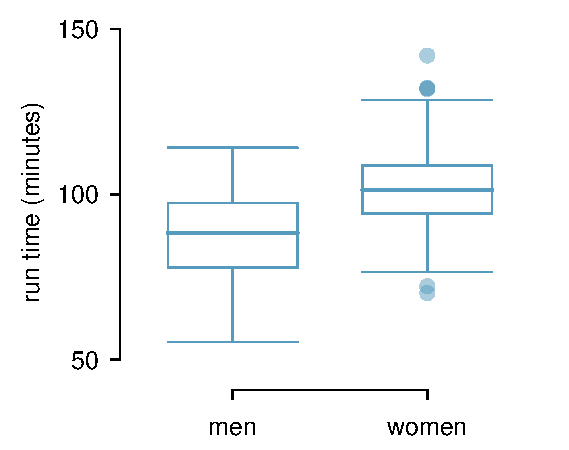
\includegraphics[width=0.5\textwidth]{05/figures/cbrRunTimesMenWomen/cbrRunTimesMenWomen}
\caption{Side-by-side box plots for the sample of 2009 Cherry Blossom Run participants.}
\label{cbrRunTimesMenWomen}
\end{figure}

The two samples are independent of one-another, so the data are not paired. Instead a point estimate of the difference in average 10 mile times for men and women, $\mu_w - \mu_m$, can be found using the two sample means:
\begin{eqnarray*}
\bar{x}_{w} - \bar{x}_{m}\ =\ 102.13 - 87.65\ =\ 14.48
\end{eqnarray*}
%Because we are examining two simple random samples from less than 10\% of the population, each sample contains at least 30 observations, and neither distribution is strongly skewed, we can safely conclude the sampling distribution of each sample mean is nearly normal. Finally, because each sample is independent of the other (e.g. the data are not paired), we can conclude that the difference in sample means can be modeled using a normal distribution.\footnote{Probability theory guarantees that the difference of two independent normal random variables is also normal. Because each sample mean is nearly normal and observations in the samples are independent, we are assured the difference is also nearly normal.}

%\begin{termBox}{\tBoxTitle{Conditions for normality of $\bar{x}_1 - \bar{x}_2$}
%If the sample means, $\bar{x}_1$ and $\bar{x}_2$, each meet the criteria for having nearly normal sampling distributions and the observations in the two samples are independent, then the difference in sample means, $\bar{x}_1 - \bar{x}_2$, will have a sampling distribution that is nearly normal.}
%\end{termBox}


Suppose we are told by an expert in sports science that the standard deviations of the time taken
to complete 10 mile marathons is approximately equal.
We can also visually see that $s_{w} \approx s_{m}$.
As such we need to calculate the pooled sample variance. Using Equation~\eqref{eqnPooledVariance} we get
\begin{align*}
s_{p}^{2} 	& = \frac{ (n_{w}-1)s_{w}^{2} + (n_{m}-1)s_{m}^{2} }{n_{m} + n_{m} - 2}	\\
		& = \frac{ (55 -1)15.2^{2} + (45-1)12.5^{2} }{45 + 55 - 2}	\\
		& = 197.46
\end{align*}

We can quantify the variability in the point estimate, $\bar{x}_{w} - \bar{x}_{m}$, using the following formula for its standard error:
\index{standard error!difference in means}
%\begin{eqnarray*}
%%SE_{\bar{x}_{w} - \bar{x}_{m}} = \sqrt{\frac{\sigma_{w}^2}{n_{w}} + \frac{\sigma_{m}^2}{n_{m}}}
%SE_{\bar{x}_{w} - \bar{x}_{m}} = \sqrt{\frac{s_{w}^2}{n_{w}} + \frac{s_{m}^2}{n_{m}}}
%\end{eqnarray*}
%We usually estimate this standard error using standard deviation estimates  based on the samples:
%\begin{align*}
%SE_{\bar{x}_{w} - \bar{x}_{m}}
%	&= \sqrt{\frac{\sigma_{w}^2}{n_{w}} + \frac{\sigma_{m}^2}{n_{m}}} \\
%	&\approx \sqrt{\frac{s_{w}^2}{n_{w}} + \frac{s_{m}^2}{n_{m}}}
%	= \sqrt{\frac{15.2^2}{55} + \frac{12.5^2}{45}} = 2.77
%\end{align*}
%\begin{align*}
%SE_{\bar{x}_{w} - \bar{x}_{m}}
%	&= \sqrt{\frac{s_{w}^2}{n_{w}} + \frac{s_{m}^2}{n_{m}}} 	\\
%	&= \sqrt{\frac{15.2^2}{55} + \frac{12.5^2}{45}} 			\\
%	&= 2.77
%\end{align*}

\begin{align*}
SE_{\bar{x}_{w} - \bar{x}_{m}}
&=	\sqrt{ s_{p}^{2} \bigg( \frac{1}{n_{1}} + \frac{1}{n_{2}} \bigg)}	\\
&=	\sqrt{197.46 \bigg( \frac{1}{55} + \frac{1}{45} \bigg)}			\\
%&=	2.824573
&=	2.82
\end{align*}

%Because each sample has at least 30 observations ($n_{w} = 55$ and $n_{m} = 45$), this substitution using the sample standard deviation tends to be very good.

\index{point estimate!difference of means|)}




%When the data indicate that the point estimate $\bar{x}_{1} - \bar{x}_{2}$ comes from a nearly normal distribution, we can construct a confidence interval for the difference in two means from the framework built in Chapter~\ref{foundationsForInference}. 
Here a point estimate, $\bar{x}_{w} - \bar{x}_{m} = 14.48$, is associated with %a normal model with
standard error $SE=2.82$. 
The next step is to find the appropriate value from the $t$ tables.
For a 95\% confidence interval, $\alpha/2 = 0.025$.
The appropriate value of the degrees of freedom $d$ that we should use is
%\begin{align*}
%d = \min(45-1, \, 55-1) = 44
%\end{align*}
\begin{align*}
n_{w} + n_{m} - 2 = 55 + 45 - 2 = 98
\end{align*}
This means that the value we use from the $t$ tables is $t_{0.025, 98}$.
However Table~\ref{tDistributionTable} does not contain values for 98 degrees of freedom.
Therefore we round down to the nearest available degrees of freedom in the table which
are 90 degrees of freedom.
The value of $t_{(0.025, 90)} = 1.99$.
Our 95\% confidence interval is therefore
%Using this information, the general confidence interval formula may be applied in an attempt to capture the true difference in means, in this case using a 95\% confidence level:
\begin{eqnarray*}
%\text{point estimate}\  \pm \ z^{\star}SE \quad\to\quad 14.48\  \pm \ 1.96\times 2.77 \quad\to\quad (9.05, 19.91)
14.48\  \pm \ 1.99 \times 2.82 = (8.87, \, 20.09)
\end{eqnarray*}
Based on the samples, we are 95\% confident that men ran, on average, between 8.87 and 20.09 minutes faster than women in the 2012 Cherry Blossom Run.\\












\subsection{On paired data}
\label{pairedData}
\label{sectionPairedData}


A confidence interval on \term{paired data} (also referred to as a term{matched pairs}) is performed when we have two measurements which depend on each of the units sampled.
Our population is the population of differences and our parameter of interest is the
mean difference between $\mu_{d}$.

\begin{termBox}{\tBoxTitle{Paired data}
Two sets of observations are \emph{paired} if each observation in one set has a special correspondence or connection with exactly one observation in the other data set.}
\end{termBox}


With paired data we take the difference in the two measurements for each unit.
This gives us a set of differences.
We then calculate the sample mean and sample standard deviation for these differences
which we label as $\bar{x}_{d}$ and $s_{d}$ respectively\footnote{We use a subscript of $d$ to indicate that we our statistics are on a set of differences. The calculations of the mean and standard deviation are still the same.}.
We then use $\bar{x}_{d}$ and $s_{d}$ to create a confidence interval on the mean difference.


\begin{termBox}{\tBoxTitle{A $(100 - \alpha)$\% confidence interval on paired data}
\begin{equation}
\bar{x}_{d}	 ~~ \pm ~~  t_{(\alpha / 2, \, n-1)}  \bigg( \frac{ s_{d} }{ \sqrt{n} } \bigg)\label{eqnCIPairedData}\\
\end{equation}
}
\end{termBox}

Notice that Equation~\ref{eqnCIPairedData} is essentially the equation for constructing a confidence interval on the mean when $\sigma$ is not known which is
given by Equation~\ref{eqnCISigmaNOTKnown}.
We have however introduced different labels that fit this context.

\index{paired data|(}
\index{data!textbooks|(}

The example we will use to illustrate Equation~\eqref{eqnCIPairedData} is whether textbooks are actually cheaper online? We compare the price of textbooks at the bookstore
of the University of California, Los Angeles (UCLA) and prices at %Amazon.com. 
%\href{http://www.amazon.com}{\color{black}\textbf{Amazon.com}}.
\href{http://www.amazon.com}{Amazon.com}.
Seventy-three UCLA courses were randomly sampled in Spring 2010, representing less than 10\% of all UCLA courses.\footnote{When a class had multiple books, only the most expensive text was considered.} A portion of this data set is shown in Table~\ref{textbooksDF}.

\begin{table}[H]
\centering
\begin{tabular}{rllrrr}
  \hline
 & Department & Course & UCLA & \href{http://www.amazon.com}{Amazon.com} & Difference \\ 
  \hline
1 & Am Ind &  C170 & 27.67 & 27.95 & -0.28 \\ 
  2 & Anthro & 9 & 40.59 & 31.14 & 9.45 \\ 
  3 & Anthro & 135T & 31.68 & 32.00 & -0.32 \\ 
  4 & Anthro & 191HB & 16.00 & 11.52 & 4.48 \\ 
$\vdots$ & $\vdots$ & $\vdots$ & $\vdots$ & $\vdots$ & $\vdots$ \\
  72 & Wom Std & M144 & 23.76 & 18.72 & 5.04 \\ 
  73 & Wom Std & 285 & 27.70 & 18.22 & 9.48 \\ 
   \hline
\end{tabular}
\captionsetup{width=0.6\textwidth}
\caption{Six entries from the \data{textbooks} data set.}
\label{textbooksDF}
\end{table}
%library(openintro); library(xtable); data(textbooks); xtable(textbooks[c(1:5, nrow(textbooks) - 1:0),])

%\subsection{Paired observations and samples}

Each textbook has two corresponding prices in the data set: one for the UCLA bookstore and one for Amazon. Therefore, each textbook price from the UCLA bookstore has a natural correspondence with a textbook price from Amazon. 
%When two sets of observations have this special correspondence, they are said to be \term{paired}.
Since these two sets of observations have this special correspondence, they can be considered as paired.

To analyze paired data, it is often useful to look at the difference in outcomes of each pair of observations. In the \data{textbook} data set, we look at the difference in prices, which is represented as the \var{diff} variable in the \data{textbooks} data. Here the differences are taken as
\begin{eqnarray*}
\text{UCLA price} - \text{Amazon price}
\end{eqnarray*}
for each book. It is important that we always subtract using a consistent order; here Amazon prices are always subtracted from UCLA prices. A histogram of these differences is shown in Figure~\ref{diffInTextbookPricesS10}. Using differences between paired observations is a common and useful way to analyze paired data.

The distribution of differences, shown in Figure~\ref{diffInTextbookPricesS10}, is %strongly 
slighlty skewed, but this amount of skew is reasonable for this sized data set ($n=73$). 


\begin{figure}[H]
\centering
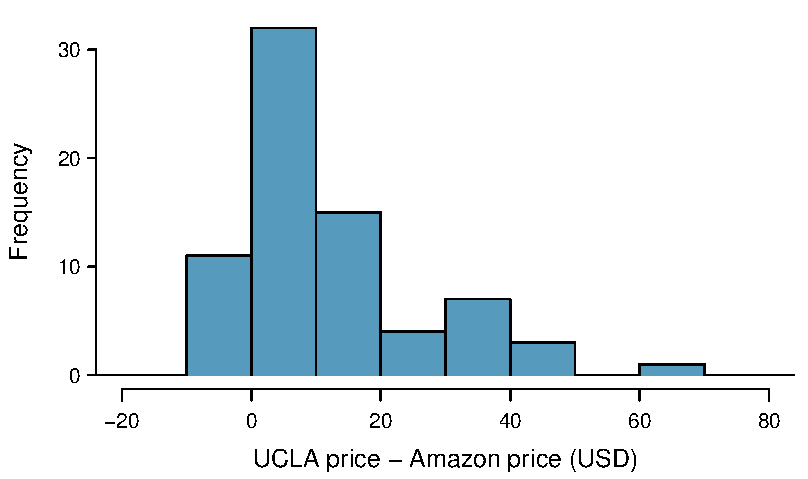
\includegraphics[width=0.9\textwidth]{05/figures/textbooksS10/diffInTextbookPricesS10}
\captionsetup{width=0.6\textwidth}
\caption{Histogram of the difference in price for each book sampled. These data are %strongly
slighlty skewed.\index{skew!example: strong}}
\label{diffInTextbookPricesS10}
\end{figure}

%\begin{exercise}
%The first difference shown in Table~\ref{textbooksDF} is computed as $27.67-27.95=-0.28$. Verify the differences are calculated correctly for observations 2 and 3.\footnote{Observation 2: $40.59 - 31.14 = 9.45$. Observation 3: $31.68 - 32.00 = -0.32$.}
%\end{exercise}

%\subsection{Inference for paired data}

%To analyze a paired data set, we use the exact same tools that we developed in Chapter~\ref{foundationsForInference}. Now we apply them to the differences in the paired observations.
A summary of the column of differences in Table~\ref{textbooksDF} is given in
Table~\ref{textbooksSummaryStats} below.

\begin{table}[H]
\centering
\begin{tabular}{ccccc}
\hline
$n_{_{d}}$	&\hspace{3mm}& $\bar{x}_{_{d}}$	&\hspace{3mm}& $s_{_{d} }$ \vspace{1mm}\\
73			&			& 12.76			&			& 14.26 \\
\hline
\end{tabular}
\captionsetup{width=0.6\textwidth}
\caption{Summary statistics for the price differences. There were 73 books, so there are 73 differences.}
\label{textbooksSummaryStats}
\end{table}

%\begin{example}{Set up and implement a hypothesis test to determine whether, on average, there is a difference between Amazon's price for a book and the UCLA bookstore's price.}
%\label{htForDiffInUCLAAndAmazonTextbookPrices}
%There are two scenarios: there is no difference or there is some difference in average prices. The \emph{no difference} scenario is always the null hypothesis:
%\begin{itemize}
%\setlength{\itemsep}{0mm}
%\item[$H_0$:] $\mu_{d}=0$. There is no difference in the average textbook price.
%\item[$H_A$:] $\mu_{d} \neq 0$. There is a difference in average prices.
%\end{itemize}

%Can the normal model be used to describe the sampling distribution of $\bar{x}_{d}$? We must check that the differences meet the conditions established in Chapter~\ref{foundationsForInference}. The observations are based on a simple random sample from less than 10\% of all books sold at the bookstore, so independence is reasonable; there are more than 30 differences; and 

%Because all three conditions are reasonably satisfied, we can conclude the sampling distribution of $\bar{x}_{d}$ is nearly normal and our estimate of the standard error will be reasonable.

We compute the standard error associated with $\bar{x}_{d}$ using the standard deviation of the differences ($s_{_{d}}=14.26$) and the number of differences ($n=73$):

%$$SE_{\bar{x}_{d}} = \frac{s_{d}}{\sqrt{n_{d}}} = \frac{14.26}{\sqrt{73}} = 1.67$$
\begin{equation*}
SE_{\bar{x}_{d}} = \frac{s_{d}}{\sqrt{n}} = \frac{14.26}{\sqrt{73}} = 1.67
\end{equation*}

%To visualize the p-value, the sampling distribution of $\bar{x}_{d}$ is drawn as though $H_0$ is true, which is shown in Figure~\ref{textbooksS10HTTails}. The p-value is represented by the two (very) small tails.
%\begin{figure}[H]
%\centering
%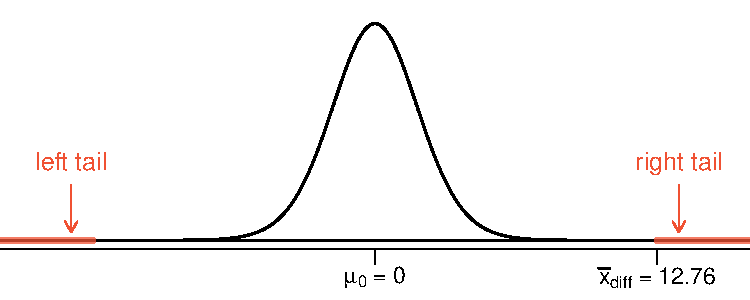
\includegraphics[width=0.65\textwidth]{05/figures/textbooksS10/textbooksS10HTTails}
%\caption{Sampling distribution for the mean difference in book prices, if the true average difference is zero.}
%\label{textbooksS10HTTails}
%\end{figure}

%To find the tail areas, we compute the test statistic, which is the Z score of $\bar{x}_{d}$ under the null condition that the actual mean difference is 0:
%$$Z = \frac{\bar{x}_{d} - 0}{SE_{x_{d}}} = \frac{12.76 - 0}{1.67} = 7.59$$
%This Z score is so large it isn't even in the table, which ensures the single tail area will be 0.0002 or smaller. Since the p-value corresponds to both tails in this case and the normal distribution is symmetric, the p-value can be estimated as twice the one-tail area:
%$$\text{p-value} = 2\times (\text{one tail area}) \approx 2\times 0.0002 = 0.0004$$
%Because the p-value is less than 0.05, we reject the null hypothesis. We have found convincing evidence that Amazon is, on average, cheaper than the UCLA bookstore for UCLA course textbooks.
%%\end{example}

%\begin{exercise}
%Create a 95\% confidence interval for the average price difference between books at the UCLA bookstore and books on Amazon.\footnote{Conditions have already verified and the standard error computed in Example~\ref{htForDiffInUCLAAndAmazonTextbookPrices}. To find the interval, identify $z^{\star}$ (1.96 for 95\% confidence) and plug it, the point estimate, and the standard error into the confidence interval formula:
%$$\text{point estimate} \ \pm\ z^{\star}SE \quad\to\quad 12.76 \ \pm\ 1.96\times 1.67 \quad\to\quad (9.49, 16.03)$$
%We are 95\% confident that Amazon is, on average, between \$9.49 and \$16.03 cheaper than the UCLA bookstore for UCLA course books.}

Let's now create a 95\% confidence interval for the average price difference between books at the UCLA bookstore and books on Amazon.
We need the value of $t_{\alpha/2, n-1} = t_{0.025, 72}$.
However our the $t$ distribution table in Chapter~\ref{tDistributionTable} does not 
provide values for 72 degrees of freedom.
Therefore we round down to 70 degrees of freedom and use
$t_{\alpha/2, n-1} = t_{0.025, 72} = 1.99$.
%To find the interval, identify $z^{\star}$ (1.96 for 95\% confidence) and plug it, the point estimate, and the standard error into the confidence interval formula:
Our 95\% confidence interval on the true difference between the bookstore and 
\href{http://www.amazon.com}{Amazon.com} is
%$$\text{point estimate} \ \pm\ z^{\star}SE \quad\to\quad 12.76 \ \pm\ 1.96\times 1.67 \quad\to\quad (9.49, 16.03)$$

\begin{equation*}
12.76 \ \pm\ 1.99\times 1.67 = (9.44,  16.08)
\end{equation*}

We are 95\% confident that Amazon is, on average, between \$9.49 and \$16.03 cheaper than the UCLA bookstore for UCLA course books.
%}

\index{data!textbooks|)}
\index{paired data|)}

%\end{exercise}







\hfill\\

{\color{red}{FILL UP}}

\vfill


\pagebreak



\subsection{On a difference of two proportions}
\label{differenceOfTwoProportions}


In this Chapter we analyze the method to make conclusions about the difference in two population proportions: $p_1 - p_2$. 

%{\color{red}{We consider three examples. In the first, we compare the approval of the 2010 healthcare law under two different question phrasings. In the second application, a company weighs whether they should switch to a higher quality parts manufacturer. In the last example, we examine the cancer risk to dogs from the use of yard herbicides.}}
We examine an example in which we compare the approval of the 2010 healthcare law under two different question phrasings.

In our investigations, we first identify a reasonable point estimate of $p_1 - p_2$ based on the sample. You may have already guessed its form: $\hat{p}_1 - \hat{p}_2$\index{point estimate!difference of proportions}. Next, in each example we verify that the point estimate follows the normal model by checking certain conditions. Finally, we compute the estimate's standard error and apply our inferential framework.


The formula for constructing a confidence interval on a difference of proportions is

\begin{termBox}{\tBoxTitle{A $(100 - \alpha)$\% confidence interval on $p_{1} - p_{2}$ when 
$\sigma_{1}$ and $\sigma_{2}$ are not known and $\sigma_{1} = \sigma_{2}$}
\begin{equation}
\hat{p}_{1} - \hat{p}_{2}	~~ \pm ~~		z_{\alpha / 2}  
\sqrt{ \frac{p_1(1-p_1)}{n_1}  +  \frac{p_2(1-p_2)}{n_2} }\label{eqnCIDiffProps}
\end{equation}
}
\end{termBox}


In Equation~\eqref{eqnCIDiffProps}, 
%$\sqrt{ \frac{p_1(1-p_1)}{n_1}  +  \frac{p_2(1-p_2)}{n_2} }$ 
%is the standard error of proportion and
%$z_{\alpha / 2} \sqrt{ \frac{p_1(1-p_1)}{n_1}  +  \frac{p_2(1-p_2)}{n_2} }$
%is the margin of error.
everything under the square root sign is the standard error of proportion and
this value multiplied by $z_{\alpha / 2}$ is the margin of error.

%\subsection{Sample distribution of the difference of two proportions}

%We must check two conditions before applying the normal model to $\hat{p}_1 - \hat{p}_2$. First, the sampling distribution for each sample proportion must be nearly normal, and secondly, the samples must be independent. Under these two conditions, the sampling distribution of $\hat{p}_1 - \hat{p}_2$ may be well approximated using the normal model.
%
%\begin{termBox}{\tBoxTitle{Conditions for the sampling distribution of $\hat{p}_1 - \hat{p}_2$ to be normal}
%The difference $\hat{p}_1 - \hat{p}_2$ tends to follow a normal model when
%\begin{itemize}
%\setlength{\itemsep}{0mm}
%\item each proportion separately follows a normal model, and
%\item the two samples are independent of each other.
%\end{itemize}
%The standard error of the difference in sample proportions is
%\index{standard error!difference in proportions}
%\begin{eqnarray}
%SE_{\hat{p}_1 - \hat{p}_2}
%	= \sqrt{SE_{\hat{p}_1}^2 + SE_{\hat{p}_2}^2}
%	= \sqrt{\frac{p_1(1-p_1)}{n_1} + \frac{p_2(1-p_2)}{n_2}}
%\label{seForDiffOfProp}
%\end{eqnarray}
%where $p_1$ and $p_2$ represent the population proportions, and $n_1$ and $n_2$ represent the sample sizes.}
%\end{termBox}

%For the difference in two means, the standard error formula took the following form:
%\begin{eqnarray*}
%SE_{\bar{x}_{1} - \bar{x}_{2}} = \sqrt{SE_{\bar{x}_1}^2 + SE_{\bar{x}_2}^2}
%\end{eqnarray*}
%The standard error for the difference in two proportions takes a similar form. The reasons behind this similarity are rooted in the probability theory of Section~\ref{randomVariablesSection}, which is described for this context in Exercise~\vref{derivingSEForDiffOfTwoMeansExercise}.

%\subsection{Intervals and tests for $p_1 -p_2$}

Let's now do an example.
In the setting of confidence intervals, the sample proportions are used to verify the success-failure condition and also compute standard error, just as was the case with a single proportion.
%\begin{example}{
The way a question is phrased can influence a person's response. For example, Pew Research Center conducted a survey with the following question:\footnote{\href{http://www.people-press.org/2012/03/26/public-remains-split-on-health-care-bill-opposed-to-mandate/}{www.people-press.org/2012/03/26/public-remains-split-on-health-care-bill-opposed-to-mandate/}. Sample sizes for each polling group are approximate.}
\begin{quote}
As you may know, by 2014 nearly all Americans will be required to have health insurance. [People who do not buy insurance will pay a penalty] while [People who cannot afford it will receive financial help from the government]. Do you approve or disapprove of this policy?
\end{quote}
\index{data!health care|(}For each randomly sampled respondent, the statements in brackets were randomized: either they were kept in the order given above, or the two statements were reversed. Table~\ref{pewPollResultsForRandomizedStatementOrdering} shows the results of this experiment. 
We shall create and interpret a 90\% confidence interval of the difference in approval.
%}

\begin{table}[H]
\centering
\begin{tabular}{p{50mm}c p{13mm}p{14mm}p{16.5mm}c}
	&\ & Sample size ($n_i$) & Approve law (\%)	& Disapprove law (\%)	& Other \\
\hline
``people who cannot afford it will receive financial help from the government'' is given second \vspace{2.5mm}
	& & 771	& 47	& 49	& 3 \\
``people who do not buy it will pay a penalty'' is given second
	& & 732	& 34	& 63	& 3 \\
\hline
\end{tabular}
\captionsetup{width=0.8\textwidth}
\caption{Results for a Pew Research Center poll where the ordering of two statements in a question regarding healthcare were randomized.\vspaceB{-2mm}}
\label{pewPollResultsForRandomizedStatementOrdering}
\end{table}

%First the conditions must be verified. Because each group is a simple random sample from less than 10\% of the population, the observations are independent, both within the samples and between the samples. The success-failure condition also holds for each sample. Because all conditions are met, the normal model can be used for the point estimate of the difference in support, where 
We will let
$p_1$ corresponds to the original ordering and $p_2$ to the reversed ordering.
A point estimate for the difference in proportions is
%$$\hat{p}_{1} - \hat{p}_{2} = 0.47 - 0.34 = 0.13$$
\begin{equation*}
\hat{p}_{1} - \hat{p}_{2} = 0.47 - 0.34 = 0.13
\end{equation*}
The standard error may be computed from Equation~\eqref{eqnCIDiffProps}%Equation~\eqref{seForDiffOfProp} 
using the sample proportions:
%$$SE \approx \sqrt{\frac{0.47(1-0.47)}{771} + \frac{0.34(1-0.34)}{732}} = 0.025$$
\begin{equation*}
SE = \sqrt{\frac{0.47(1-0.47)}{771} + \frac{0.34(1-0.34)}{732}} = 0.025
\end{equation*}
For a 90\% confidence interval, $z_{\alpha/2} = 1.65$.
Therefore our 90\% confidence interval on the difference of proportions is:
%$$\text{point estimate} \ \pm\ z^{\star}SE \quad \to \quad 0.13 \ \pm\ 1.65 \times  0.025 \quad \to \quad (0.09, 0.17)$$
\begin{equation*}
0.13 \ \pm\ 1.65 \times  0.025 = (0.09, 0.17)
\end{equation*}
The interpretation of this interval is that 
we are 90\% confident that the approval rating for the 2010 healthcare law changes between 9\% and 17\% due to the ordering of the two statements in the survey question. The Pew Research Center reported that this modestly large difference suggests that the opinions of much of the public are still fluid on the health insurance mandate.
\index{data!health care|)}

%\end{example}

%\begin{exercise}\label{carWheelGearManufacturer}
%A remote control car company is considering a new manufacturer for wheel gears. The new manufacturer would be more expensive but their higher quality gears are more reliable, resulting in happier customers and fewer warranty claims. However, management must be convinced that the more expensive gears are worth the conversion before they approve the switch. If there is strong evidence of a more than 3\% improvement in the percent of gears that pass inspection, management says they will switch suppliers, otherwise they will maintain the current supplier. Set up appropriate hypotheses for the test.\footnote{$H_0$: The higher quality gears will pass inspection no more than 3\% more frequently than the standard quality gears. $p_{highQ} - p_{standard} = 0.03$. $H_A$: The higher quality gears will pass inspection more than 3\% more often than the standard quality gears. $p_{highQ} - p_{standard} > 0.03$.}
%\end{exercise}
%
%\begin{example}{The quality control engineer from Exercise~\ref{carWheelGearManufacturer} collects a sample of gears, examining 1000 gears from each company and finds that 899 gears pass inspection from the current supplier and 958 pass inspection from the prospective supplier. Using these data, evaluate the hypothesis setup of Exercise~\ref{carWheelGearManufacturer} using a significance level of 5\%.}
%First, we check the conditions. The sample is not necessarily random, so to proceed we must assume the gears are all independent; for this sample we will suppose this assumption is reasonable, but the engineer would be more knowledgeable as to whether this assumption is appropriate. The success-failure condition also holds for each sample. Thus, the difference in sample proportions, $0.958-0.899=0.059$, can be said to come from a nearly normal distribution.
%
%The standard error can be found using Equation~\eqref{seForDiffOfProp}:
%$$SE = \sqrt{\frac{0.958(1-0.958)}{1000} + \frac{0.899(1-0.899)}{1000}} = 0.0114$$
%In this hypothesis test, the sample proportions were used. We will discuss this choice more in Section~\ref{pooledHTForProportionsSection}.
%
%Next, we compute the test statistic and use it to find the p-value, which is depicted in Figure~\ref{gearsTwoSampleHTPValueQC}.
%$$Z = \frac{\text{point estimate} - \text{null value}}{SE} = \frac{0.059 - 0.03}{0.0114} = 2.54$$
%Using the normal model for this test statistic, we identify the right tail area as 0.006. Since this is a one-sided test, this single tail area is also the p-value, and we reject the null hypothesis because 0.006 is less than 0.05. That is, we have statistically significant evidence that the higher quality gears actually do pass inspection more than 3\% as often as the currently used gears. Based on these results, management will approve the switch to the new supplier.
%\end{example}
%
%\begin{figure}[H]
%\centering
%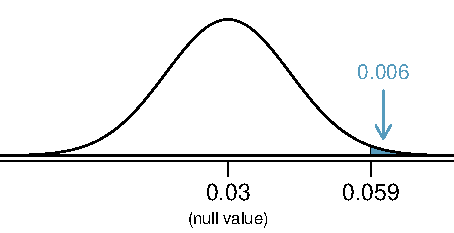
\includegraphics[width=0.5\textwidth]{06/figures/gearsTwoSampleHTPValueQC/gearsTwoSampleHTPValueQC}
%\caption{Distribution of the test statistic if the null hypothesis was true. The p-value is represented by the shaded area.}
%\label{gearsTwoSampleHTPValueQC}
%\end{figure}








\subsection{Assumptions}

\subsubsection{On a difference of two means}

For confidence intervals on $\mu_{1} - \mu_{2}$ the assumptions that are required are the following

\begin{enumerate}
\item	Data from both samples are taken from random samples from large populations.
\item	The sample size of each sample should be less than 10\% of their corresponding population.
\item	Observations in a sample must be independent of each observation from the same sample.
\item	Observations in a sample must be independent of each observation from the other sample.
\item	Both populations are approximately normally distributed.
\end{enumerate}




\subsubsection{On paired data}

For confidence intervals on $\mu_{d}$ the assumptions that are required are the following

\begin{enumerate}
\item	Two measurements from each observation are dependent on the unit from which they were measured.
\item	The sample size should be less than 10\% of the population.
\item	Measurements on each unit are independent of each measurement on other units.
\item	The population of differences is normally distributed.
\item	For the Pooled Method : The two populations have the same variance.\footnote{This assumption is called the assumption of \emph{homogeneity} of variance}\\
	For Welch's Interval	: The two populations do not have the same variance.\footnote{This assumption is called the assumption of \emph{heterogeneity} of variance}
\end{enumerate}






\subsubsection{On a difference of two proportions}

For confidence intervals on $p_{1} - p_{2}$ the assumptions that are required are the following

\begin{enumerate}
\item	Data from both samples are taken from random samples from large populations.
\item	Observations in a sample must be independent of each observation from the same sample.
\item	Observations in a sample must be independent of each observation from the other sample.
\item	$n_{1}p_{1} \geq 10$ and $n_{1}(1-p_{1}) \geq 10$ 
	as well as $n_{2}p_{2} \geq 10$ and $n_{2}(1-p_{2}) \geq 10$.
	\label{npAssumpForTwoSampleDiffInProp}
%	\footenotesize{Similar to assumption~\ref{npAssumpForOneSampleProp} in Chapter~ }\ref{sectionAssumpOnProp} }
\end{enumerate}

Since we do not know $p_{1}$ or $p_{2}$ we can attempt to verify assumption~\ref{npAssumpForTwoSampleDiffInProp} by estimating 
$p_{1}$ with $\hat{p}_{1}$ as well as estimating
$p_{2}$ with $\hat{p}_{2}$.
As such we can check whether
$n_{1}\hat{p}_{1} \geq 10$ and $n_{1}(1-\hat{p}_{1}) \geq 10$ 
as well
$n_{2}\hat{p}_{2} \geq 10$ and $n_{2}(1-\hat{p}_{2}) \geq 10$ 
(Similar to the check we can perform in assumption~\ref{npAssumpForOneSampleProp}
in Chapter~\ref{sectionAssumpOnProp})





%\subsection{Changing the confidence level}
%\label{changingTheConfidenceLevelSection}
%
%\index{confidence interval!confidence level|(}
%
%
%
%
%
%The normal approximation is crucial to the precision of these confidence intervals. Section~\ref{cltSection} provides a more detailed discussion about when the normal model can safely be applied. When the normal model is not a good fit, we will use alternative distributions that better characterize the sampling distribution.
%
%\begin{termBox}{\tBoxTitle{Conditions for $\bar{x}$ being nearly normal and $SE$ being accurate\label{terBoxOfCondForXBarBeingNearlyNormalAndSEBeingAccurate}}
%Important conditions to help ensure the sampling distribution of $\bar{x}$ is nearly normal and the estimate of SE sufficiently accurate:
%\begin{itemize}
%\item The sample observations are independent.
%\item The sample size is large: $n\geq30$ is a good rule of thumb.
%\item The distribution of sample observations is not strongly skewed.
%\end{itemize}
%Additionally, the larger the sample size, the more lenient we can be with the sample's skew.}
%\end{termBox}
%
%Verifying independence is often the most difficult of the conditions to check, and the way to check for independence varies from one situation to another. However, we can provide simple rules for the most common scenarios. 
%
%\begin{tipBox}{\tipBoxTitle{How to verify sample observations are independent}
%Observations in a simple random sample consisting of less than 10\% of the population are independent.}
%\end{tipBox}
%
%\begin{caution}
%{Independence for random processes and experiments}
%{If a sample is from a random process or experiment, it is important to verify the observations from the process or subjects in the experiment are nearly independent and maintain their independence throughout the process or experiment. Usually subjects are considered independent if they undergo random assignment in an experiment.}
%\end{caution}
%
%
%% WARNING !!!!
%% EOCE 4.9 (as of 2nd Edition) references the results of this exercise
%
%\begin{termBox}{\tBoxTitle{Confidence interval for any confidence level}
%If the point estimate follows the normal model with standard error $SE$, then a confidence interval for the population parameter is
%\begin{eqnarray*}
%\text{point estimate}\ \pm\ z^{\star} SE
%\end{eqnarray*}
%where $z^{\star}$ corresponds to the confidence level selected.}
%\end{termBox}
%
%Figure~\ref{choosingZForCI} provides a picture of how to identify $z^{\star}$ based on a confidence level. We select $z^{\star}$ so that the area between -$z^{\star}$ and $z^{\star}$ in the normal model corresponds to the confidence level. 
%
%\begin{termBox}{\tBoxTitle{Margin of error}
%\label{marginOfErrorTermBox}In a confidence interval, $z^{\star}\times SE$ is called the \term{margin of error}.}
%\end{termBox}
%




%
%%\subsection{Interpreting confidence intervals}
%
%
%
%
%
%
%
%
%
%\subsection[Nearly normal population with known SD (special topic)]{Nearly normal population with known SD (special topic)}
%\label{nearlyNormalPopWithKnownSD}
%
%\index{Central Limit Theorem!normal data|(}
%
%In rare circumstances we know important characteristics of a population. For instance, we might know a population is nearly normal and we may also know its parameter values. Even so, we may still like to study characteristics of a random sample from the population. Consider the conditions required for modeling a sample mean using the normal distribution:
%\begin{enumerate}
%\setlength{\itemsep}{0mm}
%\item[(1)] The observations are independent.
%\item[(2)] The sample size $n$ is at least 30.
%\item[(3)] The data distribution is not strongly skewed.
%\end{enumerate}
%These conditions are required so we can adequately estimate the standard deviation and so we can ensure the distribution of sample means is nearly normal. However, if the population is known to be nearly normal, the sample mean is always nearly normal (this is a special case of the Central Limit Theorem). If the standard deviation is also known, then conditions (2) and (3) are not necessary for those data.
%
%\begin{example}{The heights of male seniors in high school closely follow a normal distribution $N(\mu=70.43, \sigma=2.73)$, where the units are inches.\footnote{These values were computed using the USDA Food Commodity Intake Database.} If we randomly sampled the heights of five male seniors, what distribution should the sample mean follow?}\label{simpleSampleOfFiveMaleSeniors}
%The population is nearly normal, the population standard deviation is known, and the heights represent a random sample from a much larger population, satisfying the independence condition. Therefore the sample mean of the heights will follow a nearly normal distribution with mean $\mu=70.43$ inches and standard error $SE=\sigma/\sqrt{n} = 2.73/\sqrt{5}=1.22$ inches.
%\end{example}
%
%\begin{termBox}{\tBoxTitle{Alternative conditions for applying the normal distribution to model the sample mean}
%If the population of cases is known to be nearly normal and the population standard deviation $\sigma$ is known, then the sample mean $\bar{x}$ will follow a nearly normal distribution $N(\mu, \sigma/\sqrt{n})$ if the sampled observations are also independent.}
%\end{termBox}
%
%Sometimes the mean changes over time but the standard deviation remains the same. In such cases, a sample mean of small but nearly normal observations paired with a known standard deviation can be used to produce a confidence interval for the current population mean using the normal distribution.
%
%\begin{example}{Is there a connection between height and popularity in high school? Many students may suspect as much, but what do the data say? Suppose the top 5 nominees for prom king at a high school have an average height of 71.8 inches. Does this provide strong evidence that these seniors' heights are not representative of all male seniors at their high school?}
%If these five seniors are height-representative, then their heights should be like a random sample from the distribution given in Example~\ref{simpleSampleOfFiveMaleSeniors}, $N\left(\mu=70.43, \sigma = 2.73\right)$, and the sample mean should follow $N\left(\mu=70.43, \sigma/\sqrt{n} = 1.22\right)$. Formally we are conducting what is called a \emph{hypothesis test}, which we will discuss in greater detail during the next section. We are weighing two possibilities:
%\begin{itemize}
%\setlength{\itemsep}{0mm}
%\item[$H_0$:] The prom king nominee heights are representative; $\bar{x}$ will follow a normal distribution with mean 70.43 inches and standard error 1.22 inches.
%\item[$H_A$:] The heights are not representative; we suspect the mean height is different from 70.43 inches.
%\end{itemize}
%If there is strong evidence that the sample mean is not from the normal distribution provided in $H_0$, then that suggests the heights of prom king nominees are not a simple random sample (i.e. $H_A$ is true). We can look at the Z score of the sample mean to tell us how unusual our sample is. If $H_0$ is true:
%\begin{align*}
%Z = \frac{\bar{x} - \mu}{\sigma/\sqrt{n}} = \frac{71.8 - 70.43}{1.22} = 1.12
%\end{align*}
%A Z score of just 1.12 is not very unusual (we typically use a threshold of $\pm2$ to decide what is unusual), so there is not strong evidence against the claim that the heights are representative. This does not mean the heights are actually representative, only that this very small sample does not necessarily show otherwise.
%\end{example}
%
%\begin{tipBox}{\tipBoxTitle{Relaxing the nearly normal condition}
%As the sample size becomes larger, it is reasonable to \emph{slowly} relax the nearly normal assumption on the data when dealing with small samples. By the time the sample size reaches 30, the data must show strong skew for us to be concerned about the normality of the sampling distribution.}
%\index{Central Limit Theorem!normal data|)}
%\end{tipBox}
%
%
%%__________________
%\section{Hypothesis testing}
%\label{hypothesisTesting}
%
%\index{hypothesis testing|(}
%
%Is the typical US runner getting faster or slower over time? We consider this question in the context of the Cherry Blossom Run, comparing runners in 2006 and 2012. Technological advances in shoes, training, and diet might suggest runners would be faster in 2012. An opposing viewpoint might say that with the average body mass index on the rise, people tend to run slower. In fact, all of these components might be influencing run time.
%
%In addition to considering run times in this section, we consider a topic near and dear to most students: sleep. A recent study found that college students average about 7 hours of sleep per night.\footnote{\urlwofont{http://theloquitur.com/?p=1161}} However, researchers at a rural college are interested in showing that their students sleep longer than seven hours on average. We investigate this topic in Section~\ref{pValue}.
%
%\subsection{Hypothesis testing framework}
%
%The average time for all runners who finished the Cherry Blossom Run in 2006 was 93.29 minutes (93 minutes and about 17 seconds). We want to determine if the \data{run10Samp} data set provides strong evidence that the participants in 2012 were faster or slower than those runners in 2006, versus the other possibility that there has been no change.\footnote{While we could answer this question by examining the entire population data (\data{run10}), we only consider the sample data (\data{run10Samp}), which is more realistic since we rarely have access to population data.} We simplify these three options into two competing \termsub{hypotheses}{hypothesis}:
%\begin{itemize}
%\setlength{\itemsep}{0mm}
%\item[$H_0$:] The average 10 mile run time was the same for 2006 and 2012.
%\item[$H_A$:] The average 10 mile run time for 2012 was \emph{different} than that of 2006.
%\end{itemize}
%We call $H_0$\marginpar[\raggedright\vspace{6mm}
%
%$H_0$\\\footnotesize null hypothesis\vspace{3mm}\\\normalsize $H_A$\\\footnotesize alternative\\ hypothesis]{\raggedright\vspace{6mm}
%
%$H_0$\\\footnotesize null hypothesis\vspace{3mm}\\\normalsize $H_A$\\\footnotesize alternative\\ hypothesis} the null hypothesis and $H_A$ the alternative hypothesis.
%
%\begin{termBox}{\tBoxTitle{Null and alternative hypotheses}
%{\small The \term{null hypothesis ($H_0$)} often represents either a skeptical perspective or a claim to be tested. The \term{alternative hypothesis ($H_A$)} represents an alternative claim under consideration and is often represented by a range of possible parameter values.}}
%\end{termBox}
%
%The null hypothesis often represents a skeptical position or a perspective of no difference. The alternative hypothesis often represents a new perspective, such as the possibility that there has been a change. 
%
%\begin{tipBox}{\tipBoxTitle{Hypothesis testing framework}
%The skeptic will not reject the null hypothesis ($H_0$), unless the evidence in favor of the alternative hypothesis ($H_A$) is so strong that she rejects $H_0$ in favor of $H_A$.}
%\end{tipBox}
%
%The hypothesis testing framework is a very general tool, and we often use it without a second thought. If a person makes a somewhat unbelievable claim, we are initially skeptical. However, if there is sufficient evidence that supports the claim, we set aside our skepticism and reject the null hypothesis in favor of the alternative. The hallmarks of hypothesis testing are also found in the US court system. 
%
%\begin{exercise} \label{hypTestCourtExample}
%A US court considers two possible claims about a defendant: she is either innocent or guilty. If we set these claims up in a hypothesis framework, which would be the null hypothesis and which the alternative?\footnote{The jury considers whether the evidence is so convincing (strong) that there is no reasonable doubt regarding the person's guilt; in such a case, the jury rejects innocence (the null hypothesis) and concludes the defendant is guilty (alternative hypothesis).}
%\end{exercise}
%
%Jurors examine the evidence to see whether it convincingly shows a defendant is guilty. Even if the jurors leave unconvinced of guilt beyond a reasonable doubt, this does not mean they believe the defendant is innocent. This is also the case with hypothesis testing: \emph{even if we fail to reject the null hypothesis, we typically do not accept the null hypothesis as true}. Failing to find strong evidence for the alternative hypothesis is not equivalent to accepting the null hypothesis.
%
%In the example with the Cherry Blossom Run, the null hypothesis represents no difference in the average time from 2006 to 2012. The alternative hypothesis represents something new or more interesting: there was a difference, either an increase or a decrease. These hypotheses can be described in mathematical notation using $\mu_{12}$ as the average run time for 2012:
%\begin{itemize}
%\setlength{\itemsep}{0mm}
%\item[$H_0$:] $\mu_{12} = 93.29$ %93.28864
%\item[$H_A$:] $\mu_{12} \neq 93.29$
%\end{itemize}
%where $93.29$ minutes (93 minutes and about 17 seconds) is the average 10 mile time for all runners in the 2006 Cherry Blossom Run. Using this mathematical notation, the hypotheses can now be evaluated using statistical tools. We call 93.29 the \term{null value} since it represents the value of the parameter if the null hypothesis is true. We will use the \data{run10Samp} data set to evaluate the hypothesis test.
%
%
%\subsection{Testing hypotheses using confidence intervals}
%\label{utilizingOurCI}
%
%We can start the evaluation of the hypothesis setup by comparing 2006 and 2012 run times using a point estimate from the 2012 sample: $\bar{x}_{12} = 95.61$ minutes. This estimate suggests the average time is actually longer than the 2006 time, 93.29 minutes. However, to evaluate whether this provides strong evidence that there has been a change, we must consider the uncertainty associated with $\bar{x}_{12}$.
%
%We learned in Section~\ref{variabilityInEstimates} that there is fluctuation from one sample to another, and it is very unlikely that the sample mean will be exactly equal to our parameter; we should not expect $\bar{x}_{12}$ to exactly equal $\mu_{12}$. Given that $\bar{x}_{12} = 95.61$, it might still be possible that the population average in 2012 has remained unchanged from 2006. The difference between $\bar{x}_{12}$ and 93.29 could be due to \emph{sampling variation}, i.e. the variability associated with the point estimate when we take a random sample.
%
%In Section~\ref{confidenceIntervals}, confidence intervals were introduced as a way to find a range of plausible values for the population mean. Based on \data{run10Samp}, a 95\% confidence interval for the 2012 population mean, $\mu_{12}$, was calculated as
%\begin{eqnarray*}
%(92.45, 98.77)
%\end{eqnarray*}
%Because the 2006 mean, 93.29, falls in the range of plausible values, we cannot say the null hypothesis is implausible. That is, we failed to reject the null hypothesis, $H_0$. 
%
%\begin{tipBox}{\tipBoxTitle{Double negatives can sometimes be used in statistics}
%In many statistical explanations, we use double negatives. For instance, we might say that the null hypothesis is \emph{not implausible} or we \emph{failed to reject} the null hypothesis. Double negatives are used to communicate that while we are not rejecting a position, we are also not saying it is correct.}
%\end{tipBox}
%
%\begin{example}{Next consider whether there is strong evidence that the average age of runners has changed from 2006 to 2012 in the Cherry Blossom Run. In 2006, the average age was 36.13 years, and in the 2012 \data{run10Samp} data set, the average was 35.05 years with a standard deviation of 8.97 years for 100 runners.}
%First, set up the hypotheses:
%\begin{itemize}
%\setlength{\itemsep}{0mm}
%\item[$H_0$:] The average age of runners has not changed from 2006 to 2012, $\mu_{age} = 36.13$.
%\item[$H_A$:] The average age of runners has changed from 2006 to 2012, $\mu_{age} \neq 36.13$.
%\end{itemize}
%We have previously verified conditions for this data set. The normal model may be applied to $\bar{y}$ and the estimate of $SE$ should be very accurate. Using the sample mean and standard error, we can construct a 95\% confidence interval for $\mu_{age}$ to determine if there is sufficient evidence to reject $H_0$:
%\begin{eqnarray*}
%\bar{y}\ \pm\ 1.96 \times  \frac{s}{\sqrt{100}} 
%	\quad\to\quad 35.05\ \pm\ 1.96\times 0.90 
%	\quad\to\quad (33.29, 36.81)
%\end{eqnarray*}
%This confidence interval contains the \emph{null value}, 36.13. Because 36.13 is not implausible, we cannot reject the null hypothesis. We have not found strong evidence that the average age is different than 36.13 years.
%\end{example}
%
%%\index{data!run10Samp|)}
%%\index{data!run10|)}
%
%
%
%
%
%
%
%
%
%
%
%
%\begin{exercise} \label{htForHousingExpenseForCommunityCollege650}
%Colleges frequently provide estimates of student expenses such as housing. A consultant hired by a community college claimed that the average student housing expense was \$650 per month. What are the null and alternative hypotheses to test whether this claim is accurate?\footnote{$H_0$: The average cost is \$650 per month, $\mu = \$650$.
%
%\hspace{3.4mm}$H_A$: The average cost is different than \$650 per month, $\mu \neq \$650$.}
%\end{exercise}
%
%\begin{exercise} \label{normalDistCondForHousingExpenseForCommunityCollege650}
%The community college decides to collect data to evaluate the \$650 per month claim. They take a random sample of 75 students at their school and obtain the data represented in Figure~\ref{communityCollegeClaimedHousingExpenseDistribution}. Can we apply the normal model to the sample mean?\footnote{Applying the normal model requires that certain conditions are met. Because the data are a simple random sample and the sample (presumably) represents no more than 10\% of all students at the college, the observations are independent. The sample size is also sufficiently large ($n=75$) and the data exhibit only moderate skew. Thus, the normal model may be applied to the sample mean.}
%
%\begin{figure}
%\centering
%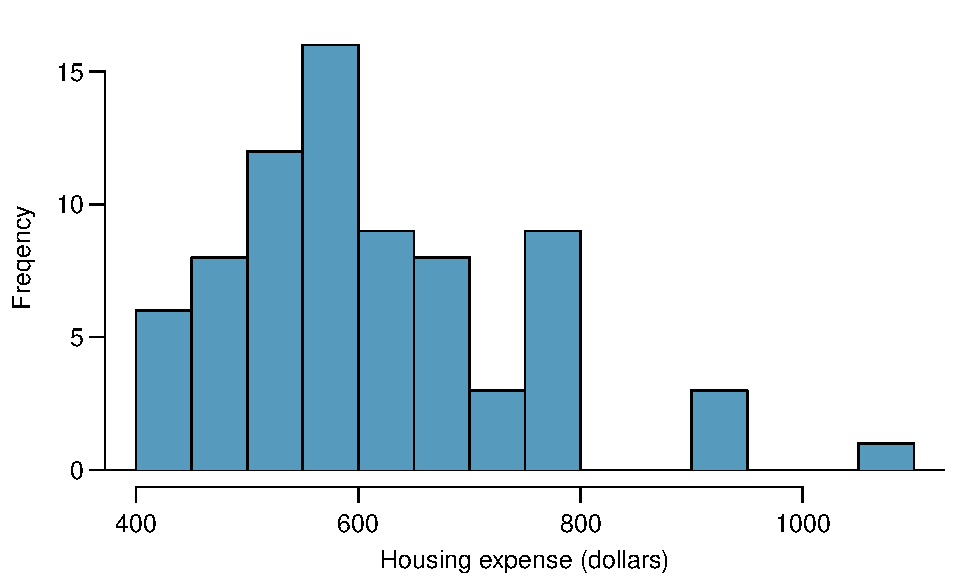
\includegraphics[width=0.85\textwidth]{04-5/figures/communityCollegeClaimedHousingExpenseDistribution/communityCollegeClaimedHousingExpenseDistribution}
%\caption{Sample distribution of student housing expense. These data are moderately skewed\index{skew!example: moderate}, roughly determined using the outliers on the~right.}
%\label{communityCollegeClaimedHousingExpenseDistribution}
%\end{figure}
%\end{exercise}
%
%
%
%\begin{example}{The sample mean for student housing is \$611.63 and the sample standard deviation is \$132.85. Construct a 95\% confidence interval for the population mean and evaluate the hypotheses of Exercise~\ref{htForHousingExpenseForCommunityCollege650}.}
%The standard error associated with the mean may be estimated using the sample standard deviation divided by the square root of the sample size. Recall that $n=75$ students were sampled.
%$$ SE = \frac{s}{\sqrt{n}} = \frac{132.85}{\sqrt{75}} = 15.34 $$
%You showed in Exercise~\ref{normalDistCondForHousingExpenseForCommunityCollege650} that the normal model may be applied to the sample mean. This ensures a 95\% confidence interval may be accurately constructed:
%$$\bar{x}\ \pm\ z^{\star} SE \quad\to\quad 611.63\ \pm\ 1.96 \times  15.34 \quad \to \quad (581.56, 641.70) $$
%Because the null value \$650 is not in the confidence interval, a true mean of \$650 is implausible and we reject the null hypothesis. The data provide statistically significant evidence that the actual average housing expense is less than \$650 per month.
%\end{example}
%
%\subsection{Decision errors}
%
%\index{hypothesis testing!decision errors|(}
%
%Hypothesis tests are not flawless. Just think of the court system: innocent people are sometimes wrongly convicted and the guilty sometimes walk free. Similarly, we can make a wrong decision in statistical hypothesis tests. However, the difference is that we have the tools necessary to quantify how often we make such errors.
%
%There are two competing hypotheses: the null and the alternative. In a hypothesis test, we make a statement about which one might be true, but we might choose incorrectly. There are four possible scenarios in a hypothesis test, which are summarized in Table~\ref{fourHTScenarios}.
%
%\begin{table}[ht]
%\centering
%\begin{tabular}{l l c c}
%& & \multicolumn{2}{c}{\textbf{Test conclusion}} \\
%  \cline{3-4}
%\vspace{-3.7mm} \\
%& & do not reject $H_0$ &  reject $H_0$ in favor of $H_A$ \\
%  \cline{2-4}
%\vspace{-3.7mm} \\
%& $H_0$ true & okay &  Type~1 Error \\
%\raisebox{1.5ex}{\textbf{Truth}} & $H_A$ true & Type 2 Error & okay \\
%  \cline{2-4}
%\end{tabular}
%\caption{Four different scenarios for hypothesis tests.}
%\label{fourHTScenarios}
%\end{table}
%
%A \term{Type~1 Error} is rejecting the null hypothesis when $H_0$ is actually true. A \term{Type~2 Error} is failing to reject the null hypothesis when the alternative is actually true.
%
%\begin{exercise} \label{whatAreTheErrorTypesInUSCourts}
%In a US court, the defendant is either innocent ($H_0$) or  guilty ($H_A$). What does a Type~1 Error represent in this context? What does a Type 2 Error represent? Table~\ref{fourHTScenarios} may be useful.\footnote{If the court makes a Type~1 Error, this means the defendant is innocent ($H_0$ true) but wrongly convicted. A Type 2 Error means the court failed to reject $H_0$ (i.e. failed to convict the person) when she was in fact guilty ($H_A$ true).}
%\end{exercise}
%
%\begin{exercise} \label{howToReduceType1ErrorsInUSCourts}
%How could we reduce the Type~1 Error rate in US courts? What influence would this have on the Type 2 Error rate?\footnote{To lower the Type~1 Error rate, we might raise our standard for conviction from ``beyond a reasonable doubt'' to ``beyond a conceivable doubt'' so fewer people would be wrongly convicted. However, this would also make it more difficult to convict the people who are actually guilty, so we would make more Type~2 Errors.}
%\end{exercise}
%
%\begin{exercise} \label{howToReduceType2ErrorsInUSCourts}
%How could we reduce the Type~2 Error rate in US courts? What influence would this have on the Type~1 Error rate?\footnote{To lower the Type~2 Error rate, we want to convict more guilty people. We could lower the standards for conviction from ``beyond a reasonable doubt'' to ``beyond a little doubt''. Lowering the bar for guilt will also result in more wrongful convictions, raising the Type~1 Error rate.}
%\end{exercise}
%
%\index{hypothesis testing!decision errors|)}
%
%Exercises~\ref{whatAreTheErrorTypesInUSCourts}-\ref{howToReduceType2ErrorsInUSCourts} provide an important lesson: if we reduce how often we make one type of error, we generally make more of the other type.
%
%Hypothesis testing is built around rejecting or failing to reject the null hypothesis. That is, we do not reject $H_0$ unless we have strong evidence. But what precisely does \emph{strong evidence} mean? As a general rule of thumb, for those cases where the null hypothesis is actually true, we do not want to incorrectly reject $H_0$ more than 5\% of the time. This corresponds to a \term{significance level}\index{hypothesis testing!significance level} of 0.05. We often write the significance level using $\alpha$\marginpar[\raggedright\vspace{-4mm}
%
%$\alpha$\\\footnotesize significance\\level of a\\hypothesis test]{\raggedright\vspace{-4mm}
%
%$\alpha$\\\footnotesize significance\\level of a\\hypothesis test} (the Greek letter \emph{alpha}\index{Greek!alpha@alpha ($\alpha$)}): $\alpha = 0.05$. We discuss the appropriateness of different significance levels in Section~\ref{significanceLevel}.
%
%If we use a 95\% confidence interval to test a hypothesis where the null hypothesis is true, we will make an error whenever the point estimate is at least 1.96 standard errors away from the population parameter. This happens about 5\% of the time (2.5\% in each tail). Similarly, using a 99\% confidence interval to evaluate a hypothesis is equivalent to a significance level of $\alpha = 0.01$.
%
%A confidence interval is, in one sense, simplistic in the world of hypothesis tests. Consider the following two scenarios:
%\begin{itemize}
%\setlength{\itemsep}{0mm}
%\item The null value (the parameter value under the null hypothesis) is in the 95\% confidence interval but just barely, so we would not reject $H_0$. However, we might like to somehow say, quantitatively, that it was a close decision.
%\item The null value is very far outside of the interval, so we reject $H_0$. However, we want to communicate that, not only did we reject the null hypothesis, but it wasn't even close. Such a case is depicted in Figure~\ref{whyWeWantPValue}.
%\end{itemize}
%In Section~\ref{pValue}, we introduce a tool called the \emph{p-value} that will be helpful in these cases. The p-value method also extends to hypothesis tests where confidence intervals cannot be easily constructed or applied.
%
%\begin{figure}[hht]
%\centering
%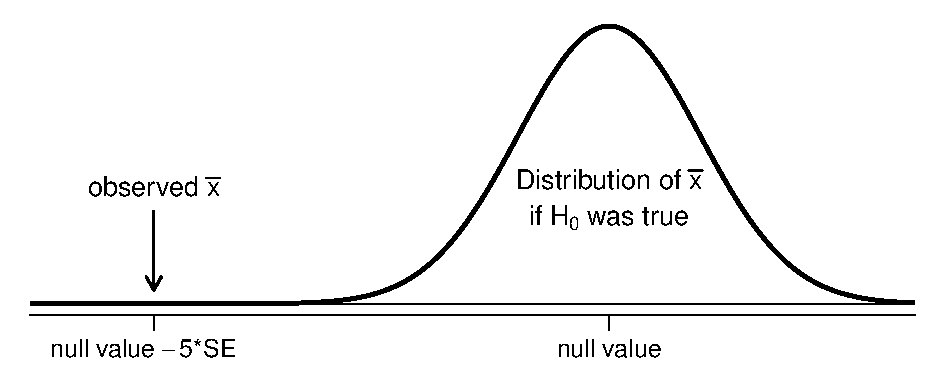
\includegraphics[width=0.75\textwidth]{04-5/figures/whyWeWantPValue/whyWeWantPValue}
%\caption{It would be helpful to quantify the strength of the evidence against the null hypothesis. In this case, the evidence is extremely strong.}
%\label{whyWeWantPValue}
%\end{figure}
%
%
%\subsection{Formal testing using p-values}
%\label{pValue}
%
%\index{hypothesis testing!p-value|(}
%
%The p-value is a way of quantifying the strength of the evidence against the null hypothesis and in favor of the alternative. Formally the \emph{p-value} is a conditional probability.
%
%\begin{termBox}{\tBoxTitle{p-value}
%The \term{p-value}\index{hypothesis testing!p-value|textbf} is the probability of observing data at least as favorable to the alternative hypothesis as our current data set, if the null hypothesis is true. We typically use a summary statistic of the data, in this chapter the sample mean, to help compute the p-value and evaluate the hypotheses.}
%\end{termBox}
%
%\index{data!school sleep|(}
%
%
%\begin{exercise} \label{skepticalPerspOfRuralSchoolSleepExercise}
%A poll by the National Sleep Foundation found that college students average about 7 hours of sleep per night. Researchers at a rural school are interested in showing that students at their school sleep longer than seven hours on average, and they would like to demonstrate this using a sample of students. What would be an appropriate skeptical position for this research?\footnote{A skeptic would have no reason to believe that sleep patterns at this school are different than the sleep patterns at another school.}
%\end{exercise}
%
%We can set up the null hypothesis for this test as a skeptical perspective: the students at this school average 7 hours of sleep per night. The alternative hypothesis takes a new form reflecting the interests of the research: the students average more than 7 hours of sleep. We can write these hypotheses as
%\begin{itemize}
%\setlength{\itemsep}{0mm}
%\item[$H_0$:] $\mu = 7$.
%\item[$H_A$:] $\mu > 7$.
%\end{itemize}
%Using $\mu > 7$ as the alternative is an example of a \term{one-sided} hypothesis test. In this investigation, there is no apparent interest in learning whether the mean is less than 7~hours.\footnote{This is entirely based on the interests of the researchers. Had they been only interested in the opposite case -- showing that their students were actually averaging fewer than seven hours of sleep but not interested in showing more than 7 hours -- then our setup would have set the alternative as $\mu < 7$.} Earlier we encountered a \term{two-sided} hypothesis where we looked for any clear difference, greater than or less than the null value.
%
%Always use a two-sided test unless it was made clear prior to data collection that the test should be one-sided. Switching a two-sided test to a one-sided test after observing the data is dangerous because it can inflate the Type~1 Error rate. 
%
%\begin{tipBox}{\tipBoxTitle{One-sided and two-sided tests}
%If the researchers are only interested in showing an increase or a decrease, but not both, use a one-sided test. If the researchers would be interested in any difference from the null value -- an increase or decrease -- then the test should be two-sided.\vspace{0.5mm}}
%\end{tipBox}
%
%\begin{tipBox}{\tipBoxTitle{Always write the null hypothesis as an equality}
%We will find it most useful if we always list the null hypothesis as an equality (e.g. $\mu = 7$) while the alternative always uses an inequality (e.g. $\mu\neq7$, $\mu>7$, or $\mu<7$).}
%\end{tipBox}
%
%The researchers at the rural school conducted a simple random sample of $n=110$ students on campus. They found that these students averaged 7.42 hours of sleep and the standard deviation of the amount of sleep for the students was 1.75 hours. A histogram of the sample is shown in Figure~\ref{histOfSleepForCollegeThatWasCheckingForMoreThan7Hours}.
%
%\begin{figure}
%\centering
%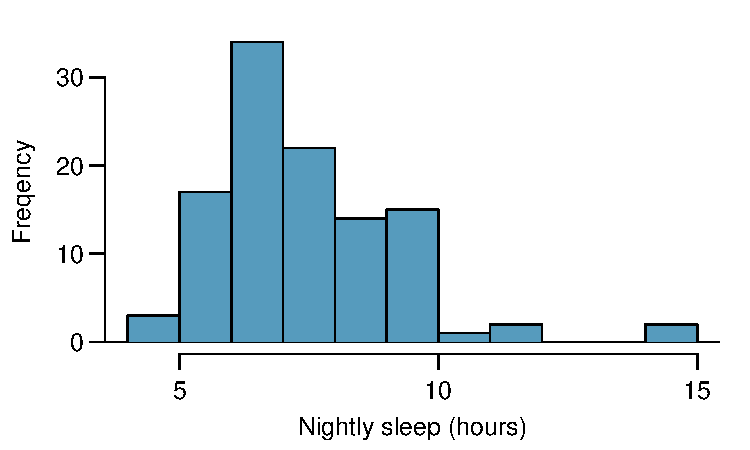
\includegraphics[height=55mm]{04-5/figures/histOfSleepForCollegeThatWasCheckingForMoreThan7Hours/histOfSleepForCollegeThatWasCheckingForMoreThan7Hours}
%\caption{Distribution of a night of sleep for 110 college students. These data are moderately skewed.\index{skew!example: moderate}}
%\label{histOfSleepForCollegeThatWasCheckingForMoreThan7Hours}
%\end{figure}
%
%Before we can use a normal model for the sample mean or compute the standard error of the sample mean, we must verify conditions. (1)~Because this is a simple random sample from less than 10\% of the student body, the observations are independent. (2)~The sample size in the sleep study is sufficiently large since it is greater than 30. (3)~The data show moderate skew in Figure~\ref{histOfSleepForCollegeThatWasCheckingForMoreThan7Hours} and the presence of a couple of outliers. This skew and the outliers (which are not too extreme) are acceptable for a sample size of $n=110$. With these conditions verified, the normal model can be safely applied to $\bar{x}$ and the estimated standard error will be very accurate.
%
%\begin{exercise} \label{findSEOfFirstSleepStudyCheckingGreaterThan7Hours}
%What is the standard deviation associated with $\bar{x}$? That is, estimate the standard error of $\bar{x}$.\footnote{The standard error can be estimated from the sample standard deviation and the sample size: $SE_{\bar{x}} = \frac{s_x}{\sqrt{n}} = \frac{1.75}{\sqrt{110}} = 0.17$.}
%\end{exercise}
%
%The hypothesis test will be evaluated using a significance level of $\alpha = 0.05$. We want to consider the data under the scenario that the null hypothesis is true. In this case, the sample mean is from a distribution that is nearly normal and has mean 7 and standard deviation of about 0.17. Such a distribution is shown in Figure~\ref{pValueOneSidedSleepStudy}.
%
%\begin{figure}[hht]
%   \centering
%   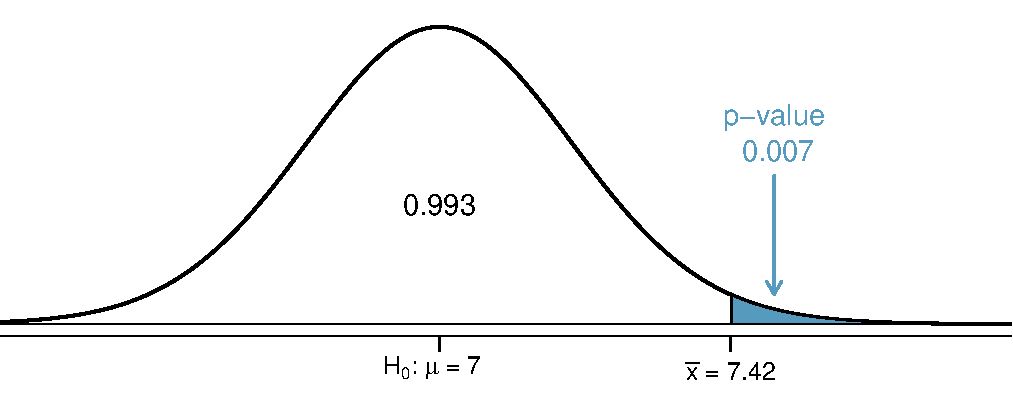
\includegraphics[width=0.73\textwidth]{04-5/figures/pValueOneSidedSleepStudy/pValueOneSidedSleepStudy}
%   \caption{If the null hypothesis is true, then the sample mean $\bar{x}$ came from this nearly normal distribution. The right tail describes the probability of observing such a large sample mean if the null hypothesis is true.}
%   \label{pValueOneSidedSleepStudy}
%\end{figure}
%
%The shaded tail in Figure~\ref{pValueOneSidedSleepStudy} represents the chance of observing such a large mean, conditional on the null hypothesis being true. That is, the shaded tail represents the p-value. We shade all means larger than our sample mean, $\bar{x} = 7.42$, because they are more favorable to the alternative hypothesis than the observed mean.
%
%We compute the p-value by finding the tail area of this normal distribution, which we learned to do in Section~\ref{normalDist}. First compute the Z score of the sample mean, $\bar{x} = 7.42$:
%\begin{eqnarray*}
%Z = \frac{\bar{x} - \text{null value}}{SE_{\bar{x}}} = \frac{7.42 - 7}{0.17} = 2.47
%\end{eqnarray*}
%Using the normal probability table, the lower unshaded area is found to be 0.993. Thus the shaded area is $1-0.993 = 0.007$. {\em If the null hypothesis is true, the probability of observing such a large sample mean for a sample of 110 students is only 0.007.}\index{p-value!interpretation example} That is, if the null hypothesis is true, we would not often see such a large mean.
%
%We evaluate the hypotheses by comparing the p-value to the significance level. Because the p-value is less than the significance level (p-value $=0.007 < 0.05=\alpha$), we reject the null hypothesis. What we observed is so unusual with respect to the null hypothesis that it casts serious doubt on $H_0$ and provides strong evidence favoring $H_A$.
%
%\begin{termBox}{\tBoxTitle{p-value as a tool in hypothesis testing}
%The p-value quantifies how strongly the data favor $H_A$ over $H_0$. A small p-value (usually $<0.05$) corresponds to sufficient evidence to reject $H_0$ in favor of $H_A$.}
%\index{hypothesis testing!p-value|)}
%\end{termBox}
%
%\begin{tipBox}{\tipBoxTitle{It is useful to first draw a picture to find the p-value}
%It is useful to draw a picture of the distribution of $\bar{x}$ as though $H_0$ was true (i.e. $\mu$ equals the null value), and shade the region (or regions) of sample means that are at least as favorable to the alternative hypothesis. These shaded regions represent the p-value.}
%\end{tipBox}
%
%The ideas below review the process of evaluating hypothesis tests with p-values:
%\begin{itemize}
%\setlength{\itemsep}{0mm}
%\item The null hypothesis represents a skeptic's position or a position of no difference. We reject this position only if the evidence strongly favors $H_A$.
%\item A small p-value means that if the null hypothesis is true, there is a low probability of seeing a point estimate at least as extreme as the one we saw. We interpret this as strong evidence in favor of the alternative.
%\item We reject the null hypothesis if the p-value is smaller than the significance level, $\alpha$, which is usually 0.05. Otherwise, we fail to reject $H_0$.
%\item We should always state the conclusion of the hypothesis test in plain language so non-statisticians can also understand the results.
%\end{itemize}
%
%The p-value is constructed in such a way that we can directly compare it to the significance level ($\alpha$) to determine whether or not to reject $H_0$. This method ensures that the Type~1 Error rate does not exceed the significance level standard. 
%
%\begin{figure}[ht]
%   \centering
%   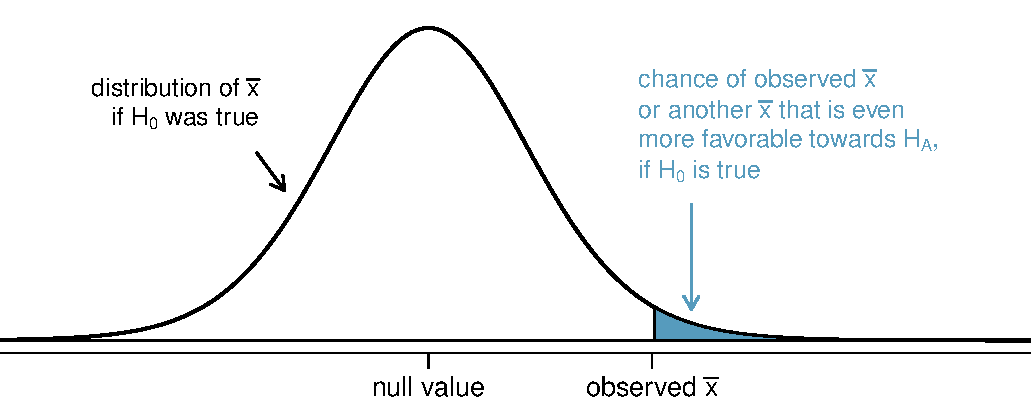
\includegraphics[width=0.9\textwidth]{04-5/figures/pValueOneSidedSleepStudyExplained/pValueOneSidedSleepStudyExplained}
%   \caption{To identify the p-value, the distribution of the sample mean is considered as if the null hypothesis was true. Then the p-value is defined and computed as the probability of the observed $\bar{x}$ or an $\bar{x}$ even more favorable to $H_A$ under this distribution.}
%   \label{pValueOneSidedSleepStudyExplained}
%\end{figure}
%
%\begin{exercise}
%If the null hypothesis is true, how often should the p-value be less than 0.05?\footnote{About 5\% of the time. If the null hypothesis is true, then the data only has a 5\% chance of being in the 5\% of data most favorable to $H_A$.}
%\index{data!school sleep|)}
%\end{exercise}
%
%\begin{exercise}
%Suppose we had used a significance level of 0.01 in the sleep study. Would the evidence have been strong enough to reject the null hypothesis? (The p-value was 0.007.) What if the significance level was $\alpha = 0.001$? \footnote{We reject the null hypothesis whenever $p$-$value < \alpha$. Thus, we would still reject the null hypothesis if $\alpha = 0.01$ but not if the significance level had been $\alpha = 0.001$.}
%\end{exercise}
%
%\begin{exercise} \label{ebayAmazonOneSidedTestExercise}
%\index{data!mario\_kart|(}
%Ebay might be interested in showing that buyers on its site tend to pay less than they would for the corresponding new item on Amazon. We'll research this topic for one particular product: a video game called \emph{Mario Kart} for the Nintendo Wii. During early October 2009, Amazon sold this game for \$46.99. Set up an appropriate (one-sided!) hypothesis test to check the claim that Ebay buyers pay less during auctions at this same time.\footnote{The skeptic would say the average is the same on Ebay, and we are interested in showing the average price is lower.
%\begin{itemize}
%\setlength{\itemsep}{0mm}
%\item[$H_0$:] The average auction price on Ebay is equal to (or more than) the price on Amazon. We write only the equality in the statistical notation: $\mu_{ebay} = 46.99$.
%\item[$H_A$:] The average price on Ebay is less than the price on Amazon, $\mu_{ebay} < 46.99$.
%\end{itemize}}
%\end{exercise}
%
%
%\begin{exercise} \label
%{exerciseFor52EbayAuctionsToExamineMarioKartLessExpensiveThanAmazonConditions}
%During early October, 2009, 52 Ebay auctions were recorded for \emph{Mario Kart}.\footnote{These data were collected by OpenIntro staff.} The total prices for the auctions are presented using a histogram in Figure~\ref{ebayMarioKartAuctionPriceHistogramFor3ConditionsExercise}, and we may like to apply the normal model to the sample mean. Check the three conditions required for applying the normal model: (1)~independence, (2)~at~least 30 observations, and (3)~the data are not strongly skewed.\footnote{(1) The independence condition is unclear. \emph{We will make the assumption that the observations are independent, which we should report with any final results.} (2) The sample size is sufficiently large: $n =52 \geq 30$. (3) The data distribution is not strongly skewed; it is approximately symmetric.}
%\end{exercise}
%
%\begin{figure}
%   \centering
%   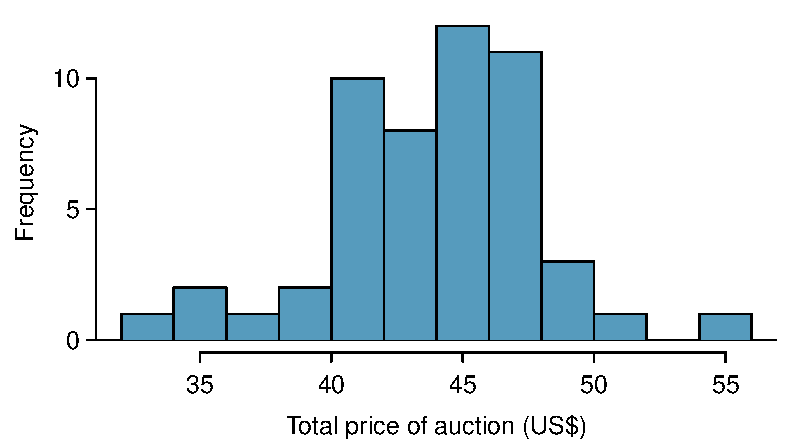
\includegraphics[width=0.68\textwidth]{04-5/figures/ebayMarioKartAuctionPriceHistogramFor3ConditionsExercise/ebayMarioKartAuctionPriceHistogramFor3ConditionsExercise}
%   \caption{A histogram of the total auction prices for 52 Ebay auctions.}
%   \label{ebayMarioKartAuctionPriceHistogramFor3ConditionsExercise}
%\end{figure}
%
%\begin{example}{The average sale price of the 52 Ebay auctions for \emph{Wii Mario Kart} was \$44.17 with a standard deviation of \$4.15. Does this provide sufficient evidence to reject the null hypothesis in Exercise~\ref{ebayAmazonOneSidedTestExercise}? Use a significance level of $\alpha = 0.01$.}
%The hypotheses were set up and the conditions were checked in Exercises~\ref{ebayAmazonOneSidedTestExercise} and~\ref{exerciseFor52EbayAuctionsToExamineMarioKartLessExpensiveThanAmazonConditions}. The next step is to find the standard error of the sample mean and produce a sketch to help find the p-value.
%\begin{eqnarray*}
%SE_{\bar{x}} = s/\sqrt{n} = 4.15/\sqrt{52} = 0.5755
%\end{eqnarray*}
%\begin{center}
%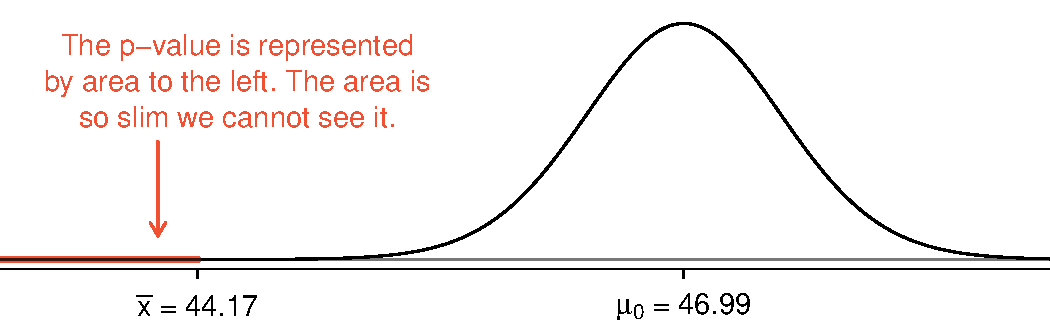
\includegraphics[height=35mm]{04-5/figures/pVForEbayAmazonComparison/pVForEbayAmazonComparison}
%\end{center}
%Because the alternative hypothesis says we are looking for a smaller mean, we shade the lower tail. We find this shaded area by using the Z score and normal probability table: $Z = \frac{44.17 - 46.99}{0.5755} = -4.90$, which has area less than 0.0002. The area is so small we cannot really see it on the picture. This lower tail area corresponds to the p-value.
%
%Because the p-value is so small -- specifically, smaller than $\alpha = 0.01$ -- this provides sufficiently strong evidence to reject the null hypothesis in favor of the alternative. The data provide statistically significant evidence that the average price on Ebay is lower than Amazon's asking price.
%\index{data!mario\_kart|)}
%\end{example}
%
%\subsection{Two-sided hypothesis testing with p-values}
%\label{twoSidedTestsWithPValues}
%
%\index{data!school sleep|(}
%
%We now consider how to compute a p-value for a two-sided test. In one-sided tests, we shade the single tail in the direction of the alternative hypothesis. For example, when the alternative had the form $\mu > 7$, then the p-value was represented by the upper tail (Figure~\ref{pValueOneSidedSleepStudyExplained}). When the alternative was $\mu < 46.99$, the p-value was the lower tail (Exercise~\ref{ebayAmazonOneSidedTestExercise}). In a two-sided test, \emph{we shade two tails} since evidence in either direction is favorable to $H_A$.
%
%\begin{exercise} \label{2ndSchSleepHypSetupExercise}
%Earlier we talked about a research group investigating whether the students at their school slept longer than 7 hours each night. Let's consider a second group of researchers who want to evaluate whether the students at their college differ from the norm of 7 hours. Write the null and alternative hypotheses for this investigation.\footnote{Because the researchers are interested in any difference, they should use a two-sided setup: $H_0: \mu = 7$, $H_A: \mu \neq 7$.}
%\end{exercise}
%
%\begin{example}{The second college randomly samples 72 students and finds a mean of $\bar{x} = 6.83$ hours and a standard deviation of $s=1.8$ hours. Does this provide strong evidence against $H_0$ in Exercise~\ref{2ndSchSleepHypSetupExercise}? Use a significance level of $\alpha=0.05$.}
%First, we must verify assumptions. (1) A simple random sample of less than 10\% of the student body means the observations are independent. (2) The sample size is 72, which is greater than 30. (3) Based on the earlier distribution and what we already know about college student sleep habits, the distribution is probably not strongly~skewed.
%
%Next we can compute the standard error ($SE_{\bar{x}} = \frac{s}{\sqrt{n}} = 0.21$) of the estimate and create a picture to represent the p-value, shown in Figure~\ref{2ndSchSleepHTExample}. Both tails are shaded. An estimate of 7.17 or more provides at least as strong of evidence against the null hypothesis and in favor of the alternative as the observed estimate, $\bar{x} = 6.83$.
%
%We can calculate the tail areas by first finding the lower tail corresponding to $\bar{x}$:
%\begin{eqnarray*}
%Z = \frac{6.83 - 7.00}{0.21} = -0.81 \quad\stackrel{table}{\rightarrow}\quad \text{left tail}=0.2090
%\end{eqnarray*}
%Because the normal model is symmetric, the right tail will have the same area as the left tail. The p-value is found as the sum of the two shaded tails:
%\begin{eqnarray*}
%\text{p-value} = \text{left tail} + \text{right tail} = 2\times(\text{left tail}) = 0.4180
%\end{eqnarray*}
%This p-value is relatively large (larger than $\alpha=0.05$), so we should not reject $H_0$. That is, if $H_0$ is true, it would not be very unusual to see a sample mean this far from 7 hours simply due to sampling variation. Thus, we do not have sufficient evidence to conclude that the mean is different than 7 hours.
%
%\index{data!school sleep|)}
%
%\begin{figure}
%   \centering
%   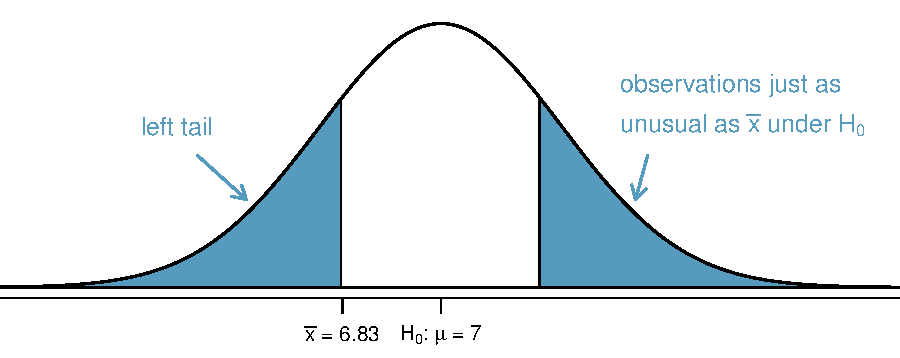
\includegraphics[width=0.9\textwidth]{04-5/figures/2ndSchSleepHTExample/2ndSchSleepHTExample}
%   \caption{$H_A$ is two-sided, so \emph{both} tails must be counted for the p-value.}
%   \label{2ndSchSleepHTExample}
%\end{figure}
%
%\end{example}
%
%\begin{example}{It is never okay to change two-sided tests to one-sided tests after observing the data. In this example we explore the consequences of ignoring this advice. Using $\alpha=0.05$, we show that freely switching from two-sided tests to one-sided tests will cause us to make twice as many Type~1 Errors as intended.} \label{swappingHypAfterDataDoublesType1ErrorRate}
%Suppose the sample mean was larger than the null value, $\mu_0$ (e.g. $\mu_0$ would represent~7 if $H_0$:~$\mu = 7$). Then if we can flip to a one-sided test, we would use $H_A$: $\mu > \mu_0$. Now if we obtain any observation with a Z score greater than 1.65, we would reject $H_0$. If the null hypothesis is true, we incorrectly reject the null hypothesis about 5\% of the time when the sample mean is above the null value, as shown in Figure~\ref{type1ErrorDoublingExampleFigure}.
%
%Suppose the sample mean was smaller than the null value. Then if we change to a one-sided test, we would use $H_A$: $\mu < \mu_0$. If $\bar{x}$ had a Z score smaller than -1.65, we would reject $H_0$. If the null hypothesis is true, then we would observe such a case about 5\% of the time.
%
%By examining these two scenarios, we can determine that we will make a Type~1 Error $5\%+5\%=10\%$ of the time if we are allowed to swap to the ``best'' one-sided test for the data. This is twice the error rate we prescribed with our significance level: $\alpha=0.05$ (!).
%
%\begin{figure}
%   \centering
%   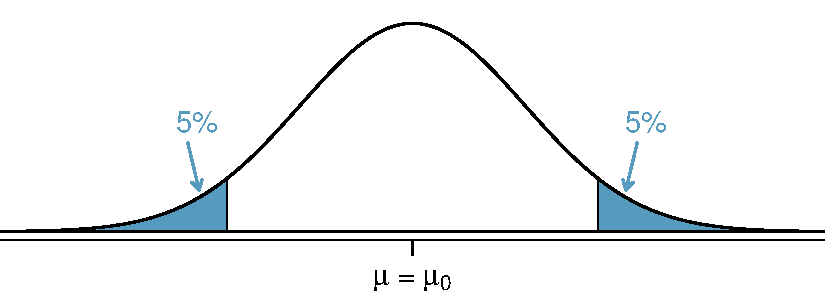
\includegraphics[width=0.7\textwidth]{04-5/figures/type1ErrorDoublingExampleFigure/type1ErrorDoublingExampleFigure}
%   \caption{The shaded regions represent areas where we would reject $H_0$ under the bad practices considered in Example~\ref{swappingHypAfterDataDoublesType1ErrorRate} when $\alpha = 0.05$.}
%   \label{type1ErrorDoublingExampleFigure}
%\end{figure}
%
%\end{example}
%
%\begin{caution}{One-sided hypotheses are allowed only \emph{before} seeing data}
%{After observing data, it is tempting to turn a two-sided test into a one-sided test. Avoid this temptation. Hypotheses must be set up \emph{before} observing the data. If~they are not, the test must be two-sided.}
%\end{caution}
%
%\subsection{Choosing a significance level}
%\label{significanceLevel}
%
%\index{hypothesis testing!significance level|(}
%\index{significance level|(}
%
%Choosing a significance level for a test is important in many contexts, and the traditional level is 0.05. However, it is often helpful to adjust the significance level based on the application. We may select a level that is smaller or larger than 0.05 depending on the consequences of any conclusions reached from the test.
%
%If making a Type~1 Error is dangerous or especially costly, we should choose a small significance level (e.g. 0.01). Under this scenario we want to be very cautious about rejecting the null hypothesis, so we demand very strong evidence favoring $H_A$ before we would reject $H_0$.
%
%If a Type 2 Error is relatively more dangerous or much more costly than a Type~1 Error, then we should choose a higher significance level (e.g. 0.10). Here we want to be cautious about failing to reject $H_0$ when the null is actually false.  We will discuss this particular case in greater detail in Section~\ref{sampleSizeAndPower}.
%
%\begin{tipBox}{\tipBoxTitle[]{Significance levels should reflect consequences of errors}
%The significance level selected for a test should reflect the consequences associated with Type~1 and Type 2 Errors.}
%\end{tipBox}
%
%\begin{example}{A car manufacturer is considering a higher quality but more expensive supplier for window parts in its vehicles. They sample a number of parts from their current supplier and also parts from the new supplier. They decide that if the high quality parts will last more than 12\% longer, it makes financial sense to switch to this more expensive supplier. Is there good reason to modify the significance level in such a hypothesis test?}
%The null hypothesis is that the more expensive parts last no more than 12\% longer while the alternative is that they do last more than 12\% longer. This decision is just one of the many regular factors that have a marginal impact on the car and company. A significance level of 0.05 seems reasonable since neither a Type~1 or Type 2 error should be dangerous or (relatively) much more expensive.
%\end{example}
%
%\begin{example}{The same car manufacturer is considering a slightly more expensive supplier for parts related to safety, not windows. If the durability of these safety components is shown to be better than the current supplier, they will switch manufacturers. Is there good reason to modify the significance level in such an evaluation?}
%The null hypothesis would be that the suppliers' parts are equally reliable. Because safety is involved, the car company should be eager to switch to the slightly more expensive manufacturer (reject $H_0$) even if the evidence of increased safety is only moderately strong. A slightly larger significance level, such as $\alpha=0.10$, might be appropriate.
%\end{example}
%
%\begin{exercise}
%A part inside of a machine is very expensive to replace. However, the machine usually functions properly even if this part is broken, so the part is replaced only if we are extremely certain it is broken based on a series of measurements. Identify appropriate hypotheses for this test (in plain language) and suggest an appropriate significance level.\footnote{Here the null hypothesis is that the part is not broken, and the alternative is that it is broken. If we don't have sufficient evidence to reject $H_0$, we would not replace the part. It sounds like failing to fix the part if it is broken ($H_0$ false, $H_A$ true) is not very problematic, and replacing the part is expensive. Thus, we should require very strong evidence against $H_0$ before we replace the part. Choose a small significance level, such as $\alpha=0.01$.}
%\end{exercise}
%
%\index{significance level|)}
%\index{hypothesis testing!significance level|)}
%\index{hypothesis testing|)}
%
%
%%%__________________
%%\section{Examining the Central Limit Theorem}
%%\label{cltSection}
%%
%%\index{Central Limit Theorem|(}
%%
%%The normal model for the sample mean tends to be very good when the sample consists of at least 30 independent observations and the population data are not strongly skewed. The Central Limit Theorem provides the theory that allows us to make this assumption.
%%
%%\begin{termBox}{\tBoxTitle{Central Limit Theorem, informal definition}
%%The distribution of $\bar{x}$ is approximately normal. The approximation can be poor if the sample size is small, but it improves with larger sample sizes.}
%%\end{termBox}
%%
%%The Central Limit Theorem states that when the sample size is small, the normal approximation may not be very good. However, as the sample size becomes large, the normal approximation improves. We will investigate three cases to see roughly when the approximation is reasonable.
%%
%%We consider three data sets: one from a \emph{uniform} distribution, one from an \emph{exponential} distribution, and the other from a \emph{log-normal} distribution. These distributions are shown in the top panels of Figure~\ref{cltSimulations}. The uniform distribution is symmetric, the exponential distribution may be considered as having moderate skew since its right tail is relatively short (few outliers), and the log-normal distribution is strongly skewed and will tend to produce more apparent outliers.\index{skew!example: moderate}\index{skew!example: strong}
%%
%%\begin{figure}
%%   \centering
%%   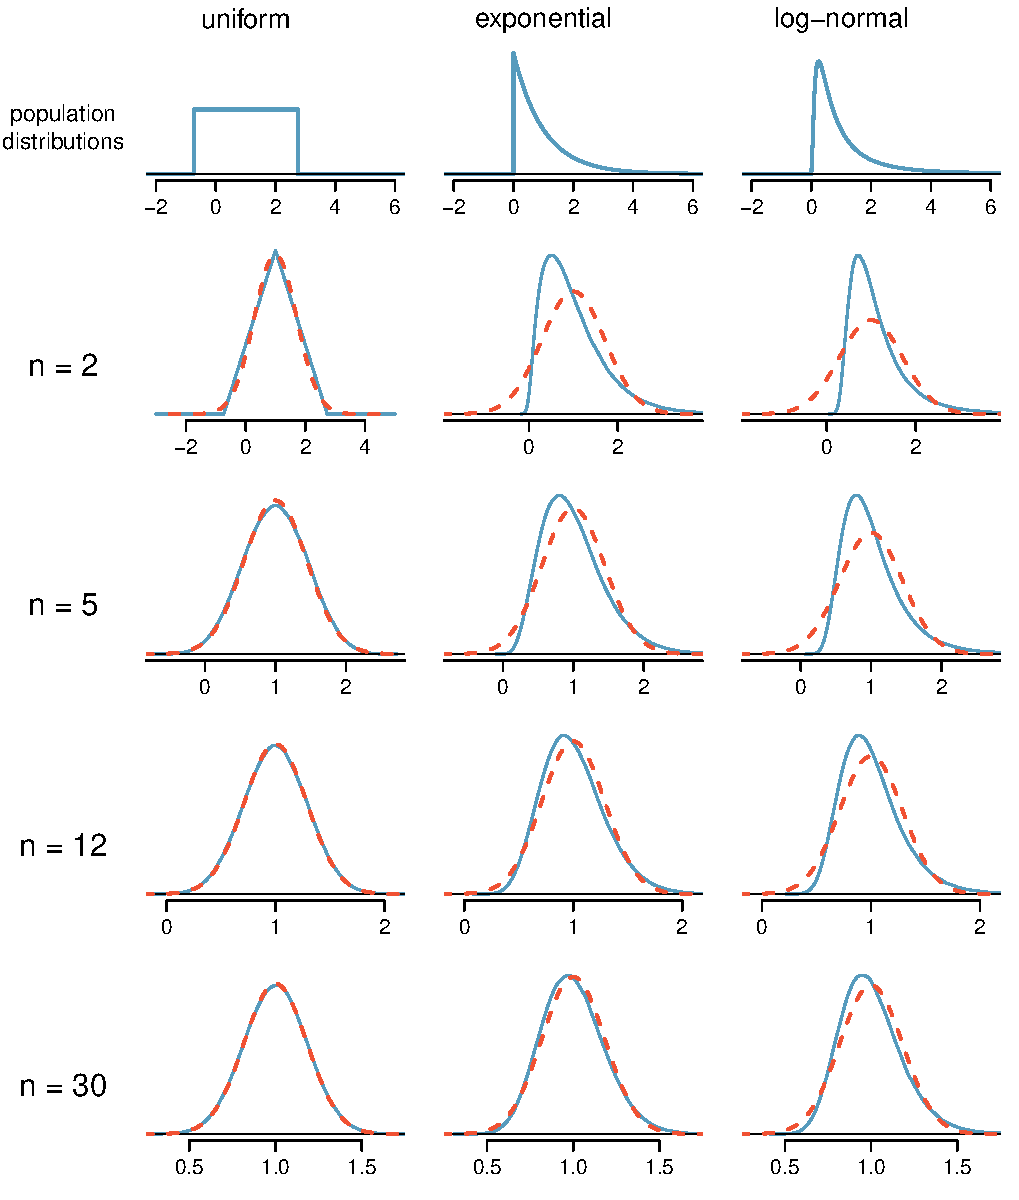
\includegraphics[width=\textwidth]{04-5/figures/cltSimulations/cltSimulationsNewest}
%%   \caption{Sampling distributions for the mean at different sample sizes and for three different distributions. The dashed red lines show normal distributions.}
%%   \label{cltSimulations}
%%\end{figure}
%%
%%The left panel in the $n=2$ row represents the sampling distribution of $\bar{x}$ if it is the sample mean of two observations from the uniform distribution shown. The dashed line represents the closest approximation of the normal distribution. Similarly, the center and right panels of the $n=2$ row represent the respective distributions of $\bar{x}$ for data from exponential and log-normal distributions.
%%
%%\begin{exercise}
%%Examine the distributions in each row of Figure~\ref{cltSimulations}. What do you notice about the normal approximation for each sampling distribution as the sample size becomes larger?\footnote{The normal approximation becomes better as larger samples are used.}
%%\end{exercise}
%%
%%\begin{example}{Would the normal approximation be good in all applications where the sample size is at least 30?}
%%Not necessarily. For example, the normal approximation for the log-normal example is questionable for a sample size of 30. Generally, the more skewed a population distribution or the more common the frequency of outliers, the larger the sample required to guarantee the distribution of the sample mean is nearly normal.
%%\end{example}
%%
%%\begin{tipBox}{\tipBoxTitle{With larger $n$, the sampling distribution of $\bar{x}$ becomes more normal}
%%As the sample size increases, the normal model for $\bar{x}$ becomes more reasonable. We can also relax our condition on skew when the sample size is very large.}
%%\end{tipBox}
%%
%%We discussed in Section~\ref{seOfTheMean} that the sample standard deviation, $s$, could be used as a substitute of the population standard deviation, $\sigma$, when computing the standard error. This estimate tends to be reasonable when $n\geq30$. We will encounter alternative distributions for smaller sample sizes in Chapters~\ref{inferenceForNumericalData} and~\ref{inferenceForCategoricalData}.
%%
%%\begin{example}{Figure~\ref{pokerProfitsCanApplyNormalToSampMean} shows a histogram of 50 observations. These represent winnings and losses from 50 consecutive days of a professional poker player. Can the normal approximation be applied to the sample mean, 90.69?}
%%We should consider each of the required conditions.
%%\begin{itemize}
%%\setlength{\itemsep}{0mm}
%%\item[(1)] These are referred to as \term{time series data}, because the data arrived in a particular sequence. If the player wins on one day, it may influence how she plays the next. To make the assumption of independence we should perform careful checks on such data. While the supporting analysis is not shown, no evidence was found to indicate the observations are not independent.
%%\item[(2)] The sample size is 50, satisfying the sample size condition.
%%\item[(3)] There are two outliers, one very extreme, which suggests the data are very strongly skewed or very distant outliers may be common for this type of data. Outliers can play an important role and affect the distribution of the sample mean and the estimate of the standard error.
%%\end{itemize}
%%Since we should be skeptical of the independence of observations and the very extreme upper outlier poses a challenge, we should not use the normal model for the sample mean of these 50 observations. If we can obtain a much larger sample, perhaps several hundred observations, then the concerns about skew and outliers would no longer apply.
%%\end{example}
%%
%%\begin{figure}[ht]
%%   \centering
%%   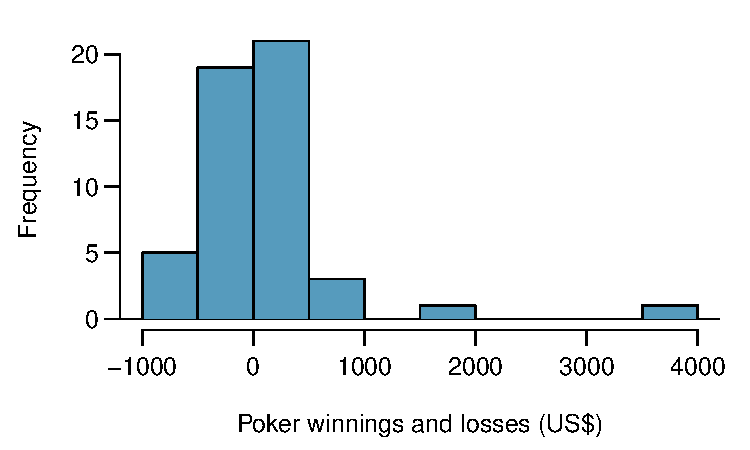
\includegraphics[height=58mm]{04-5/figures/pokerProfitsCanApplyNormalToSampMean/pokerProfitsCanApplyNormalToSampMean}
%%   \caption{Sample distribution of poker winnings. These data include some very clear outliers. These are problematic when considering the normality of the sample mean. For example, outliers are often an indicator of very strong skew\index{skew!example: very strong}.}
%%   \label{pokerProfitsCanApplyNormalToSampMean}
%%\end{figure}
%%
%%\begin{caution}
%%{Examine data structure when considering independence}
%%{Some data sets are collected in such a way that they have a natural underlying structure between observations, e.g. when observations occur consecutively. Be especially cautious about independence assumptions regarding such data sets.}
%%\end{caution}
%%
%%\begin{caution}
%%{Watch out for strong skew and outliers}
%%{Strong skew is often identified by the presence of clear outliers. If a data set has prominent outliers, or such observations are somewhat common for the type of data under study, then it is useful to collect a sample with many more than 30 observations if the normal model will be used for $\bar{x}$. There are no simple guidelines for what sample size is big enough for all situations, so proceed with caution when working in the presence of strong skew or more extreme outliers.}
%%\index{skew!strongly skewed guideline}
%%\index{Central Limit Theorem|)}
%%\end{caution}
%
%
%%__________________
%\section{Inference for other estimators}
%\label{aFrameworkForInference}
%
%The sample mean is not the only point estimate for which the sampling distribution is nearly normal. For example, the sampling distribution of sample proportions closely resembles the normal distribution when the sample size is sufficiently large. In this section, we introduce a number of examples where the normal approximation is reasonable for the point estimate. Chapters~\ref{inferenceForNumericalData} and~\ref{inferenceForCategoricalData} will revisit each of the point estimates you see in this section along with some other new statistics.
%
%We make another important assumption about each point estimate encountered in this section: the estimate is unbiased. A point estimate is \term{unbiased} if the sampling distribution of the estimate is centered at the parameter it estimates. That is, an unbiased estimate does not naturally over or underestimate the parameter. Rather, it tends to provide a ``good'' estimate. The sample mean is an example of an unbiased point estimate, as are each of the examples we introduce in this section.
%
%Finally, we will discuss the general case where a point estimate may follow some distribution other than the normal distribution. We also provide guidance about how to handle scenarios where the statistical techniques you are familiar with are insufficient for the problem at hand.
%
%
%\subsection{Confidence intervals for nearly normal point estimates}
%
%\index{confidence interval!using normal model|(}
%
%In Section~\ref{confidenceIntervals}, we used the point estimate $\bar{x}$ with a standard error $SE_{\bar{x}}$ to create a 95\% confidence interval for the population mean:
%\begin{align}
%\bar{x}\ \pm\ 1.96 \times SE_{\bar{x}}
%\label{95PercCIForMeanInGeneralizingSection}
%\end{align}
%We constructed this interval by noting that the sample mean is within 1.96 standard errors of the actual mean about 95\% of the time. This same logic generalizes to any unbiased point estimate that is nearly normal. We may also generalize the confidence level by using a place-holder $z^{\star}$.
%
%\begin{termBox}{\tBoxTitle{General confidence interval for the normal sampling distribution case}\label{generalConfidenceIntervalTermBox}%
%A confidence interval based on an unbiased and nearly normal point estimate is
%\begin{eqnarray}
%\text{point estimate}\ \pm\ z^{\star}SE
%\label{95PercGeneralCIInGeneralizingSection}
%\end{eqnarray}
%where $z^{\star}$ is selected to correspond to the confidence level, and $SE$ represents the standard error. The value $z^{\star}SE$ is called the \emph{margin of error}\index{margin of error}.}
%\end{termBox}
%
%Generally the standard error for a point estimate is estimated from the data and computed using a formula. For example, the standard error for the sample mean is
%\begin{eqnarray*}
%SE_{\bar{x}} = \frac{s}{\sqrt{n}}
%\end{eqnarray*}
%In this section, we provide the computed standard error for each example and exercise without detailing where the values came from. In future chapters, you will learn to fill in these and other details for each situation.
%
%\begin{example}{In Exercise~\vref{pointEstimateOfDifferentNetTimesBetweenGender}, we computed a point estimate for the average difference in run times between men and women: $\bar{x}_{women}-\bar{x}_{men}=14.48$ minutes. This point estimate is associated with a nearly normal distribution with standard error $SE=2.78$ minutes. What is a reasonable 95\% confidence interval for the difference in average run times?}
%\label{confIntervalForDifferenceOfRunTimeBetweenGenders}
%The normal approximation is said to be valid, so we apply Equation~\eqref{95PercGeneralCIInGeneralizingSection}:
%\begin{eqnarray*}
%\text{point estimate}\ \pm\ z^{\star} SE
%	\quad\rightarrow\quad 14.48\ \pm\ 1.96\times 2.78
%	\quad\rightarrow\quad (9.03, 19.93)
%\end{eqnarray*}
%Thus, we are 95\% confident that the men were, on average, between 9.03 and 19.93 minutes faster than women in the 2012 Cherry Blossom Run. That is, the actual average difference is plausibly between 9.03 and 19.93 minutes with 95\% confidence.
%\end{example}
%%library(openintro); library(xtable); data(run10); data(run10Samp); (x <- by(run10Samp$time, run10Samp$gender, mean)); diff(x); s <- by(run10Samp$time, run10Samp$gender, sd); n <- by(run10Samp$time, run10Samp$gender, length); sqrt(sum(s^2/n))
%
%
%\begin{example}{Does Example~\ref{confIntervalForDifferenceOfRunTimeBetweenGenders} guarantee that if a husband and wife both ran in the race, the husband would run between 9.03 and 19.93 minutes faster than the wife?}
%Our confidence interval says absolutely nothing about individual observations. It {only} makes a statement about a plausible range of values for the \emph{average} difference between all men and women who participated in the run.
%\end{example}
%
%\begin{exercise} \label{findZFor99PercConfLevelInFrameworkForInf}
%What $z^{\star}$ would be appropriate for a 99\% confidence level? For help, see Figure~\vref{choosingZForCI}.\footnote{We seek $z^{\star}$ such that 99\% of the area under the normal curve will be between the Z scores -$z^{\star}$ and $z^{\star}$. Because the remaining 1\% is found in the tails, each tail has area 0.5\%, and we can identify -$z^{\star}$ by looking up 0.0050 in the normal probability table: $z^{\star} = 2.58$. See also Figure~\vref{choosingZForCI}.}
%\end{exercise}
%
%\begin{exercise}
%The proportion of men in the \data{run10Samp} sample is $\hat{p}=0.45$. This sample meets certain conditions that ensure $\hat{p}$ will be nearly normal, and the standard error of the estimate is $SE_{\hat{p}}=0.05$. Create a 90\% confidence interval for the proportion of participants in the 2012 Cherry Blossom Run who are men.\footnote{We use $z^{\star}=1.65$ (see Exercise~\vref{find90CIForRun10AgeExercise}), and apply the general confidence interval formula:
%\begin{eqnarray*}
%\hat{p}\ \pm\ z^{\star}SE_{\hat{p}}
%	\quad\to\quad 0.45\ \pm\ 1.65\times 0.05
%	\quad\to\quad (0.3675, 0.5325)
%\end{eqnarray*}
%Thus, we are 90\% confident that between 37\% and 53\% of the participants were men.}
%\index{confidence interval!using normal model|)}
%\end{exercise}
%
%
%\subsection{Hypothesis testing for nearly normal point estimates}
%\index{hypothesis testing!using normal model|(}
%
%Just as the confidence interval method works with many other point estimates, we can generalize our hypothesis testing methods to new point estimates. Here we only consider the p-value approach, introduced in Section~\ref{pValue}, since it is the most commonly used technique and also extends to non-normal cases.
%
%\begin{termBox}{\tBoxTitle[]{Hypothesis testing using the normal model}
%\begin{enumerate}
%\setlength{\itemsep}{0mm}
%\item First write the hypotheses in plain language, then set them up in mathematical notation.
%\item Identify an appropriate point estimate of the parameter of interest.
%\item Verify conditions to ensure the standard error estimate is reasonable and the point estimate is nearly normal and unbiased.
%\item Compute the standard error. Draw a picture depicting the distribution of the estimate under the idea that $H_0$ is true. Shade areas representing the p-value.
%\item Using the picture and normal model, compute the \emph{test statistic} (Z score) and identify the p-value to evaluate the hypotheses. Write a conclusion in plain language.
%\end{enumerate}}
%\end{termBox}
%
%\begin{exercise} \label{fdaHypSetupForSulph}
%A drug called sulphinpyrazone was under consideration for use in reducing the death rate in heart attack patients. To determine whether the drug was effective, a set of 1,475 patients were recruited into an experiment and randomly split into two groups: a control group that received a placebo and a treatment group that received the new drug. What would be an appropriate null hypothesis? And the alternative?\footnote{The skeptic's perspective is that the drug does not work at reducing deaths in heart attack patients ($H_0$), while the alternative is that the drug does work ($H_A$).}
%\end{exercise}
%
%We can formalize the hypotheses from Exercise~\ref{fdaHypSetupForSulph} by letting $p_{control}$ and $p_{treatment}$ represent the proportion of patients who died in the control and treatment groups, respectively. Then the hypotheses can be written as
%\begin{eqnarray*}
%&&H_0: p_{control} = p_{treatment} \quad\text{(the drug doesn't work)} \quad \\
%&&H_A: p_{control} > p_{treatment} \quad\text{(the drug works)}
%\end{eqnarray*}
%or equivalently,
%\begin{eqnarray*}
%&&H_0: p_{control} - p_{treatment} = 0 \quad\text{(the drug doesn't work)} \quad \\
%&&H_A: p_{control} - p_{treatment} > 0 \quad\text{(the drug works)}
%\end{eqnarray*}
%Strong evidence against the null hypothesis and in favor of the alternative would correspond to an observed difference in death rates,
%\begin{eqnarray*}
%\text{point estimate} = \hat{p}_{control} - \hat{p}_{treatment}
%\end{eqnarray*}
%being larger than we would expect from chance alone. This difference in sample proportions represents a point estimate that is useful in evaluating the hypotheses. 
%
%\begin{example}{We want to evaluate the hypothesis setup from Exericse~\ref{fdaHypSetupForSulph} using data from the actual study.\footnote{Anturane Reinfarction Trial Research Group. 1980. Sulfinpyrazone in the prevention of sudden death after myocardial infarction. New England Journal of Medicine 302(5):250-256.} In the control group, 60 of 742 patients died. In the treatment group, 41 of 733 patients died. The sample difference in death rates can be summarized as
%\begin{eqnarray*}
%\text{point estimate} = \hat{p}_{control} - \hat{p}_{treatment} = \frac{60}{742} - \frac{41}{733} = 0.025
%\end{eqnarray*}
%This point estimate is nearly normal and is an unbiased estimate of the actual difference in death rates. The standard error of this sample difference is $SE = 0.013$. Evaluate the hypothesis test at a 5\% significance level: $\alpha=0.05$.}
%We would like to identify the p-value to evaluate the hypotheses. If the null hypothesis is true, then the point estimate would have come from a nearly normal distribution, like the one shown in Figure~\ref{sulphStudyFindPValueUsingNormalApprox}. The distribution is centered at zero since $p_{control}-p_{treatment}=0$ under the null hypothesis. Because a large positive difference provides evidence against the null hypothesis and in favor of the alternative, the upper tail has been shaded to represent the p-value. We need not shade the lower tail since this is a one-sided test: an observation in the lower tail does not support the alternative hypothesis.
%
%\begin{figure}[bt]
%   \centering
%   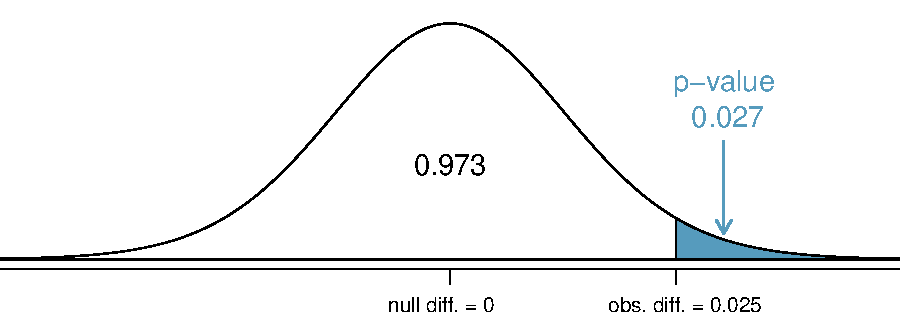
\includegraphics[height=37mm]{04-5/figures/sulphStudyFindPValueUsingNormalApprox/sulphStudyFindPValueUsingNormalApprox}
%   \caption{The distribution of the sample difference if the null hypothesis is true.}
%   \label{sulphStudyFindPValueUsingNormalApprox}
%\end{figure}
%
%The p-value can be computed by using the Z score of the point estimate and the normal probability table.
%\begin{eqnarray}
%Z = \frac{\text{point estimate} - \text{null value}}{SE_{\text{point estimate}}}
%	= \frac{0.025 - 0}{0.013} = 1.92
%\label{zScoreOfPointEstimateForSulphinpyrazoneThisIsFirstTestStatReference}
%\end{eqnarray}
%Examining $Z$ in the normal probability table, we find that the lower unshaded tail is about 0.973. Thus, the upper shaded tail representing the p-value is
%\begin{eqnarray*}
%\text{p-value} = 1-0.973 = 0.027
%\end{eqnarray*}
%Because the p-value is less than the significance level ($\alpha=0.05$), we say the null hypothesis is implausible. That is, we reject the null hypothesis in favor of the alternative and conclude that the drug is effective at reducing deaths in heart attack patients.
%\end{example}
%
%The Z score in Equation~(\ref{zScoreOfPointEstimateForSulphinpyrazoneThisIsFirstTestStatReference}) is called a \term{test statistic}. In most hypothesis tests, a test statistic is a particular data summary that is especially useful for computing the p-value and evaluating the hypothesis test. In the case of point estimates that are nearly normal, the test statistic is the Z score.
%
%\begin{termBox}{\tBoxTitle{Test statistic}
%A \emph{test statistic} is a special summary statistic that is particularly useful for evaluating a hypothesis test or identifying the p-value. When a point estimate is nearly normal, we use the Z score of the point estimate as the test statistic. In later chapters we encounter situations where other test statistics are helpful.}
%\index{hypothesis testing!using normal model|)}
%\end{termBox}
%
%
%\subsection{Non-normal point estimates}
%
%We may apply the ideas of confidence intervals and hypothesis testing to cases where the point estimate or test statistic is not necessarily normal. There are many reasons why such a situation may arise:
%\begin{itemize}
%\setlength{\itemsep}{0mm}
%\item the sample size is too small for the normal approximation to be valid;
%\item the standard error estimate may be poor; or
%\item the point estimate tends towards some distribution that is not the normal distribution.
%\end{itemize}
%For each case where the normal approximation is not valid, our first task is always to understand and characterize the sampling distribution of the point estimate or test statistic. Next, we can apply the general frameworks for confidence intervals and hypothesis testing to these alternative distributions.
%
%
%\subsection{When to retreat}
%\label{whenToRetreat}
%
%Statistical tools rely on conditions. When the conditions are not met, these tools are unreliable and drawing conclusions from them is treacherous. The conditions for these tools typically come in two forms.
%\begin{itemize}
%\setlength{\itemsep}{0mm}
%\item \textbf{The individual observations must be independent.} A random sample from less than 10\% of the population ensures the observations are independent. In experiments, we generally require that subjects are randomized into groups. If independence fails, then advanced techniques must be used, and in some such cases, inference may not be possible.
%\item \textbf{Other conditions focus on sample size and skew.} For example, if the sample size is too small, the skew too strong, or extreme outliers are present, then the normal model for the sample mean will fail.
%\end{itemize}
%Verification of conditions for statistical tools is always necessary. Whenever conditions are not satisfied for a statistical technique, there are three options. The first is to learn new methods that are appropriate for the data. The second route is to consult a statistician.\footnote{If you work at a university, then there may be campus consulting services to assist you. Alternatively, there are many private consulting firms that are also available for hire.} The third route is to ignore the failure of conditions. This last option effectively invalidates any analysis and may discredit novel and interesting findings.
%
%Finally, we caution that there may be no inference tools helpful when considering data that include unknown biases, such as convenience samples. For this reason, there are books, courses, and researchers devoted to the techniques of sampling and experimental design. See Sections~\ref{overviewOfDataCollectionPrinciples}-\ref{experimentsSection} for basic principles of data collection.
%
%
%
%%__________________
%\section{Sample size and power (special topic)}
%\label{sampleSizeAndPower}
%
%The Type 2 Error rate and the magnitude of the error for a point estimate are controlled by the sample size. Real differences from the null value, even large ones, may be difficult to detect with small samples. If we take a very large sample, we might find a statistically significant difference but the magnitude might be so small that it is of no practical value. In this section we describe techniques for selecting an appropriate sample size based on these considerations.
%
%\subsection{Finding a sample size for a certain margin of error}
%\label{findingASampleSizeForACertainME}
%
%\index{margin of error|(}
%
%Many companies are concerned about rising healthcare costs. A company may estimate certain health characteristics of its employees, such as blood pressure, to project its future cost obligations. However, it might be too expensive to measure the blood pressure of every employee at a large company, and the company may choose to take a sample instead.
%
%\begin{example}{Blood pressure oscillates with the beating of the heart, and the systolic pressure is defined as the peak pressure when a person is at rest. The average systolic blood pressure for people in the U.S. is about 130 mmHg with a standard deviation of about 25 mmHg. How large of a sample is necessary to estimate the average systolic blood pressure with a margin of error of 4 mmHg using a 95\% confidence level?}
%\label{sampleSizeComputationForSystolicBloodPressure}
%First, we frame the problem carefully. Recall that the margin of error is the part we add and subtract from the point estimate when computing a confidence interval. The margin of error for a 95\% confidence interval estimating a mean can be written as
%\begin{align*}
%ME_{95\%} = 1.96\times SE = 1.96\times\frac{\sigma_{employee}}{\sqrt{n}}
%\end{align*}
%The challenge in this case is to find the sample size $n$ so that this margin of error is less than or equal to 4, which we write as an inequality:
%\begin{align*}
%1.96\times \frac{\sigma_{employee}}{\sqrt{n}} \leq 4
%\end{align*}
%In the above equation we wish to solve for the appropriate value of $n$, but we need a value for $\sigma_{employee}$ before we can proceed. However, we haven't yet collected any data, so we have no direct estimate! Instead, we use the best estimate available to~us: the approximate standard deviation for the U.S. population, 25. To proceed and solve for $n$, we substitute 25 for $\sigma_{employee}$:
%\begin{align*}
%1.96\times \frac{\sigma_{employee}}{\sqrt{n}} \approx 1.96\times\frac{25}{\sqrt{n}}
%	&\leq 4 \\
%1.96\times\frac{25}{4} &\leq \sqrt{n} \\
%\left(1.96\times\frac{25}{4}\right)^2 &\leq n \\
%150.06 &\leq n
%\end{align*}
%This suggests we should choose a sample size of at least 151 employees. We round up because the sample size must be \emph{greater than or equal to 150.06}.
%\end{example}
%
%A potentially controversial part of Example~\ref{sampleSizeComputationForSystolicBloodPressure} is the use of the U.S. standard deviation for the employee standard deviation. Usually the standard deviation is not known. In such cases, it is reasonable to review scientific literature or market research to make an educated guess about the standard deviation.
%
%\begin{termBox}{\tBoxTitle{Identify a sample size for a particular margin of error}
%To estimate the necessary sample size for a maximum margin of error $m$, we set up an equation to represent this relationship:
%\begin{align*}
%m \geq ME = z^{\star}\frac{\sigma}{\sqrt{n}}
%\end{align*}
%where $z^{\star}$ is chosen to correspond to the desired confidence level, and $\sigma$ is the standard deviation associated with the population. Solve for the sample size,~$n$.}
%\end{termBox}
%
%Sample size computations are helpful in planning data collection, and they require careful forethought. Next we consider another topic important in planning data collection and setting a sample size: the Type 2 Error rate.
%
%\index{margin of error|)}
%
%
%\subsection{Power and the Type 2 Error rate}
%
%Consider the following two hypotheses:
%\begin{itemize}
%\setlength{\itemsep}{0.5mm}
%\item[$H_0$:] The average blood pressure of employees is the same as the national average, $\mu = 130$.
%\item[$H_A$:] The average blood pressure of employees is different than the national average, $\mu \neq 130$.
%\end{itemize}
%Suppose the alternative hypothesis is actually true. Then we might like to know, what is the chance we make a Type 2 Error? That is, what is the chance we will fail to reject the null hypothesis even though we should reject it? The answer is not obvious! If the average blood pressure of the employees is 132 (just 2 mmHg from the null value), it might be very difficult to detect the difference unless we use a large sample size. On the other hand, it would be easier to detect a difference if the real average of employees was 140.
%
%\begin{example}{Suppose the actual employee average is 132 and we take a sample of 100 individuals. Then the true sampling distribution of $\bar{x}$ is approximately $N(132, 2.5)$ (since $SE = \frac{25}{\sqrt{100}} = 2.5$). What is the probability of successfully rejecting the null hypothesis?}
%\label{computePowerIfMuIs132AndMu0Is130}
%This problem can be divided into two normal probability questions. First, we identify what values of $\bar{x}$ would represent sufficiently strong evidence to reject $H_0$. Second, we use the hypothetical sampling distribution with center $\mu=132$ to find the probability of observing sample means in the areas we found in the first step.
%
%\textbf{Step 1.} The null distribution could be represented by $N(130, 2.5)$, the same standard deviation as the true distribution but with the null value as its center. Then we can find the two tail areas by identifying the $Z$ score corresponding to the 2.5\% tails ($\pm 1.96$), and solving for $x$ in the Z score equation:
%\begin{align*}
%-1.96 = Z_1 &= \frac{x_1 - 130}{2.5}
%	&+1.96 = Z_2 &= \frac{x_2 - 130}{2.5} \\
%x_1 &= 125.1
%	&x_2 &= 134.9
%\end{align*}
%(An equally valid approach is to recognize that $x_1$ is $1.96\times SE$ below the mean and $x_2$ is $1.96\times SE$ above the mean to compute the values.) Figure~\ref{power132And141} shows the null distribution on the left with these two dotted cutoffs.
%
%\textbf{Step 2.} Next, we compute the probability of rejecting $H_0$ if $\bar{x}$ actually came from $N(132, 2.5)$. This is the same as finding the two shaded tails for the second distribution in Figure~\ref{power132And141}. We use the Z score method:
%\begin{align*}
%&Z_{left} = \frac{125.1 - 132}{2.5} = -2.76
%	&&Z_{right} = \frac{134.9 - 132}{2.5} = 1.16 \\
%&area_{left} =0.003
%	&&area_{right} =0.123
%\end{align*}
%The probability of rejecting the null mean, if the true mean is 132, is the sum of these areas: $0.003 + 0.123 = 0.126$.
%\end{example}
%
%\begin{figure}[ht]
%\centering
%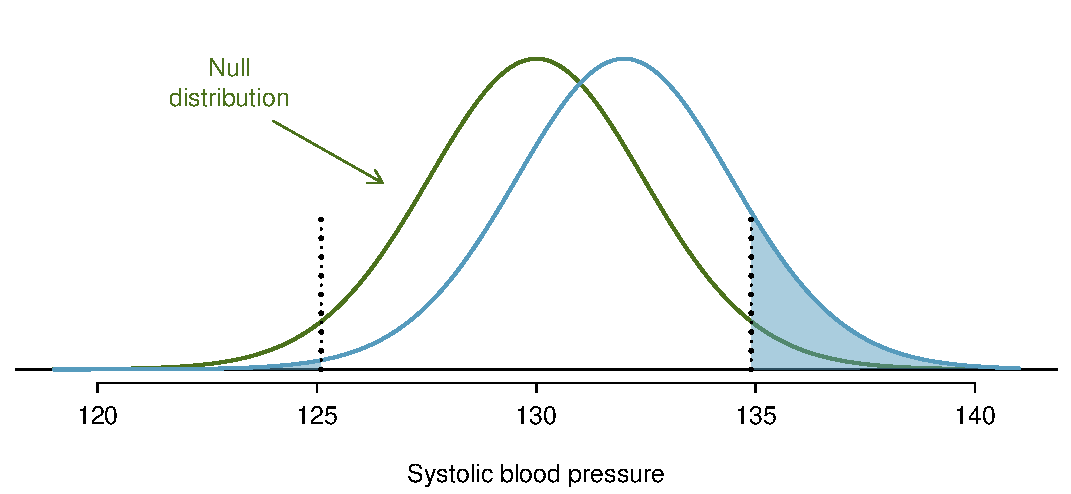
\includegraphics[width=\textwidth]{04-5/figures/power132And141/power132And141}
%\caption{The sampling distribution of $\bar{x}$ under two scenarios. Left: $N(130, 2.5)$. Right: $N(132, 2.5)$, and the shaded areas in this distribution represent the power of the test.}
%\label{power132And141}
%\end{figure}
%
%The probability of rejecting the null hypothesis is called the \term{power}. The power varies depending on what we suppose the truth might be. In Example~\ref{computePowerIfMuIs132AndMu0Is130}, the difference between the null value and the supposed true mean was relatively small, so the power was also small: only 0.126. However, when the truth is far from the null value, where we use the standard error as a measure of what is far, the power tends to increase.
%
%\begin{exercise}
%Suppose the true sampling distribution of $\bar{x}$ is centered at 140. That is, $\bar{x}$ comes from $N(140, 2.5)$. What would the power be under this scenario? It may be helpful to draw $N(140, 2.5)$ and shade the area representing power on Figure~\ref{power132And141}; use the same cutoff values identified in Example~\ref{computePowerIfMuIs132AndMu0Is130}.\footnote{Draw the distribution $N(140, 2.5)$, then find the area below 125.1 (about zero area) and above 134.9 (about 0.979). If the true mean is 140, the power is about 0.979.}
%\end{exercise}
%
%\begin{exercise}
%If the power of a test is 0.979 for a particular mean, what is the Type 2 Error rate for this mean?\footnote{The Type 2 Error rate represents the probability of failing to reject the null hypothesis. Since the power is the probability we do reject, the Type 2 Error rate will be $1-0.979 = 0.021$.}
%\end{exercise}
%
%\begin{exercise}
%Provide an intuitive explanation for why we are more likely to reject $H_0$ when the true mean is further from the null value.\footnote{Answers may vary a little. When the truth is far from the null value, the point estimate also tends to be far from the null value, making it easier to detect the difference and reject $H_0$.}
%\end{exercise}
%
%\subsection{Statistical significance versus practical significance}
%
%When the sample size becomes larger, point estimates become more precise and any real differences in the mean and null value become easier to detect and recognize. Even a very small difference would likely be detected if we took a large enough sample. Sometimes researchers will take such large samples that even the slightest difference is detected. While we still say that difference is \term{statistically significant}, it might not be \term{practically significant}.
%
%Statistically significant differences are sometimes so minor that they are not practically relevant. This is especially important to research: if we conduct a study, we want to focus on finding a meaningful result. We don't want to spend lots of money finding results that hold no practical value.
%
%The role of a statistician in conducting a study often includes planning the size of the study. The statistician might first consult experts or scientific literature to learn what would be the smallest meaningful difference from the null value. She also would obtain some reasonable estimate for the standard deviation. With these important pieces of information, she would choose a sufficiently large sample size so that the power for the meaningful difference is perhaps 80\% or 90\%. While larger sample sizes may still be used, she might advise against using them in some cases, especially in sensitive areas of research.